\documentclass{article}

% if you need to pass options to natbib, use, e.g.:
%     \PassOptionsToPackage{numbers, compress}{natbib}
% before loading neurips_2021

% ready for submission
\usepackage{neurips_2021}

% to compile a preprint version, e.g., for submission to arXiv, add add the
% [preprint] option:
%     \usepackage[preprint]{neurips_2021}

% to compile a camera-ready version, add the [final] option, e.g.:
%     \usepackage[final]{neurips_2021}

% to avoid loading the natbib package, add option nonatbib:
%    \usepackage[nonatbib]{neurips_2021}
\usepackage{colortbl}
\usepackage[utf8]{inputenc} % allow utf-8 input
\usepackage[T1]{fontenc}    % use 8-bit T1 fonts
\usepackage{hyperref}       % hyperlinks
\usepackage{url}            % simple URL typesetting
\usepackage{booktabs}       % professional-quality tables
\usepackage{amsfonts}       % blackboard math symbols
\usepackage{nicefrac}       % compact symbols for 1/2, etc.
\usepackage{microtype}      % microtypography
\usepackage{xcolor}         % colors
%!TEX root =  autocontgrlp.tex

\usepackage{multicol}
\usepackage{multirow}
\usepackage{dsfont}
\usepackage{tabularx}
%\setlength{\marginparwidth}{13mm}
\usepackage[textsize=tiny]{todonotes}
%\usepackage[disable]{todonotes}
\newcommand{\todoch}[2][]{\todo[color=blue!20!white,#1]{C: #2}}
%\usepackage{enumitem}
%\usepackage[fleqn]{amsmath}
\usepackage{amsmath}
\usepackage{mathtools}
\usepackage{graphicx}
\usepackage{times}
\usepackage{helvet}
\usepackage{courier}
\usepackage{paralist}
\usepackage{latexsym}
\usepackage{url}
\usepackage[all]{xy}
\usepackage{amsmath}
\usepackage{amssymb}
\usepackage{amsthm}
\usepackage{nccmath} % mfrac
\usepackage{comment}
%\usepackage{enumitem}
\usepackage{paralist}
\usepackage{xcolor}
%\usepackage[colorlinks=true,linkcolor=blue,citecolor=purple]{hyperref}
%\usepackage{hyperref}
\usepackage{graphicx}
\usepackage{pifont}
%\usepackage{algorithm}
%\usepackage{algorithmic}
%\usepackage{pseudocode}
%\usepackage{algpseudocode}
\usepackage{savesym}
\savesymbol{AND}
\usepackage{xspace}
\usepackage{tikz}
\usepackage{pgfplots}
\usepackage{pgf}
\usepackage{algorithm}
\usepackage{algorithmic}
\usepackage{xspace}
\usepackage{comment}
\usepackage{placeins}


%\usepackage[capitalize]{cleveref}
%\usepackage{caption}

%\usepackage{style/ssltr}
%\usepackage{style/macros}
\if0
\usetikzlibrary{intersections}
\usetikzlibrary{arrows,calc,fit,patterns,plotmarks,shapes.geometric,shapes.misc,shapes.symbols,   shapes.arrows,   shapes.callouts,   shapes.multipart,   shapes.gates.logic.US,   shapes.gates.logic.IEC,   er,   automata,   backgrounds,   chains,   topaths,   trees,   petri,   mindmap,   matrix,   calendar,   folding, fadings,   through,   positioning,   scopes,   decorations.fractals,   decorations.shapes,   decorations.text,   decorations.pathmorphing,   decorations.pathreplacing,   decorations.footprints,   decorations.markings, shadows,circuits}
\tikzstyle{decision}=[diamond,draw]
\tikzstyle{line}=[draw]
\tikzstyle{elli}=[draw,ellipse]
\tikzstyle{arrow} = [thick]
\fi
%\usepackage{subfig}

\newcommand{\rsa}{\rightsquigarrow}

\newcommand{\mb}{\mbox{ }}
\newcommand{\one}{\mathbf{1}}
\newcommand{\zero}{\mathbf{0}}
\newcommand{\nn}{\nonumber}

\newcommand{\inrdnet}{\in\R^{d_{net}}}
\newcommand{\inrdin}{\in\R^{d_{in}}}
\newcommand{\R}{\Re} %{\mathbb{R}}
\newcommand{\Rm}{\mathbf{R}_{\min}}
\newcommand{\ra}{\rightarrow}
\newcommand{\om}{\otimes}
\newcommand{\op}{\oplus}
\newcommand{\RA}{\Rightarrow}
\newcommand{\LA}{\Leftarrow}
%\newcommand{\E}{\mathbb{E}}
\newcommand{\E}[1]{\mathbb{E}\left[#1\right]}
\newcommand{\lmin}[1]{\lambda_{\min}\left(#1\right)}
\newcommand{\T}{\mathcal{T}}
\newcommand{\B}{\mathcal{B}}
\newcommand{\F}{\mathcal{F}}
\newcommand{\C}{\mathcal{C}}
\newcommand{\M}{\mathcal{M}}
\newcommand{\N}{\mathcal{N}}
\newcommand{\V}{\mathcal{V}}
\newcommand{\I}{\mathcal{I}}


\newcommand{\psiv}{\psi^{\text{v}}}
\newcommand{\psif}{\psi^{\text{f}}}

\newcommand{\kv}{K^{\text{v}}_{\Theta}}
\newcommand{\kf}{K^{\text{f}}_{\Theta}}
\newcommand{\kc}{K^{\text{cross}}_{\Theta}}

%\newcommand{\Tb}{\mathbf{\Theta}}
%\newcommand{\Tv}{\mathbf{\Theta}^v}
%\newcommand{\Tw}{\mathbf{\Theta}^w}
\newcommand{\Tv}{{\Theta}^{\text{v}}}
\newcommand{\tv}{{\theta^{\text{v}}}}
\newcommand{\Tf}{{\Theta}^{\text{f}}}
\newcommand{\tf}{{\theta}^{\text{f}}}

\newcommand{\Tdgn}{\Theta^{\text{DGN}}}


\newcommand{\din}{d_{\text{in}}}
\newcommand{\dnet}{d_{\text{net}}}
\newcommand{\dvnet}{d^{\text{v}}_{\text{net}}}
\newcommand{\dfnet}{d^{\text{f}}_{\text{net}}}
\newcommand{\ta}{\theta_\text{a}}
\newcommand{\tb}{\theta_\text{b}}
\newcommand{\tone}{\theta_\text{one}}
\newcommand{\ttwo}{\theta_\text{two}}

\newcommand{\pta}{\partial_{\ta}}
\newcommand{\ptb}{\partial_{\tb}}
%\newcommand{\Tg}{\mathbf{\Theta}^g}
\newcommand{\Tt}{\Theta}

\newcommand{\G}{\mathcal{G}}

\DeclareMathOperator{\argmin}{argmin}
\DeclareMathOperator{\argmax}{argmax}
\newcommand{\norm}[1]{\|#1\|}
\newcommand{\inorm}[1]{\|#1\|_{\infty}}
\newcommand{\snorm}[1]{\left\|#1\right\|}
\newcommand{\sinorm}[1]{\left\|#1\right\|_{\infty}}


%\newcommand{\eqdef}{\stackrel{\text{\footnotesize def}}{=}}
%\newcommand{\eqdef}{\stackrel{\Delta}{=}}
\newcommand{\eqdef}{\doteq}
\renewcommand{\eqdef}{\stackrel{def}{=}}
\newcommand{\defeq}{\doteq}

\newcommand{\eps}{\varepsilon}
\renewcommand{\epsilon}{\varepsilon}

\newcommand{\nt}{\nabla_{\Theta}}
\newcommand{\al}{\mathcal{AL}}
\newcommand{\aw}{\mathcal{AW}}
\newcommand{\ap}{\mathcal{AP}}

\newcommand{\keywords}[1]{{\bf Keywords: } #1\par}
%\newenvironment{proof}{{\bf Proof:} }{}
\newtheorem{theorem}{Theorem}[section]
\newtheorem{lemma}{Lemma}[section]
\newtheorem{claim}[theorem]{Claim}
\newtheorem{proposition}{Proposition}[section]
\newtheorem{corollary}[theorem]{Corollary}
\newtheorem{assumption}{Assumption}[section]
\newtheorem{definition}{Definition}[section]
\newtheorem{remark}{Remark}[section]
\newtheorem{identity}{Identity}[section]
\newtheorem{example}{Example}[section]
\newtheorem{note}{Note}[section]
\newtheorem{notation}{Notation}[section]
\newcommand{\alert}[1]{\textcolor{red}{#1}} 
\newcommand{\J}{\mathcal{J}}
\newcommand{\ip}[1]{\langle #1\rangle}

\def\v{\mathbf{v}}
\def\r{\mathbf{r}}
\def\p{\mathbf{p}}
\def\q{\mathbf{q}}
%\def\R{\mathrm{R}}
\def\Re{\mathbb{R}}
\def\Z{\mathbb{Z}}
\def\P{\mathcal{P}}
\def\S{\mathcal{S}}
\def\A{\mathcal{A}}
\def\X{\mathcal{X}}
\def\U{\mathcal{U}}

%\newcommand{\B}{\mathcal{B}}


\newcommand{\ith}[2][th]{$#2^{\text{#1}}$}
\newcommand{\us}[2]{\underset{#2}{#1}~}
\newcounter{subequation}[equation]
\newcommand{\thesubequationonly}{\alph{subequation}}
\renewcommand{\thesubequation}{\text{\theequation(\thesubequationonly)}}
\newcommand{\subequationitem}{\refstepcounter{subequation}(\thesubequationonly)\thinspace}

\def\mathdisplay#1{%
  \ifmmode \@badmath
  \else
    $\def\@currenvir{#1}%
    \let\dspbrk@context\z@
    \let\tag\tag@in@display \SK@equationtrue %\let\label\label@in@display
    \global\let\df@label\@empty \global\let\df@tag\@empty
    \global\tag@false
    \let\mathdisplay@push\mathdisplay@@push
    \let\mathdisplay@pop\mathdisplay@@pop
    \if@fleqn
      \edef\restore@hfuzz{\hfuzz\the\hfuzz\relax}%
      \hfuzz\maxdimen
      \setbox\z@\hbox to\displaywidth\bgroup
        \let\split@warning\relax \restore@hfuzz
        \everymath\@emptytoks \m@th $\displaystyle
    \fi
%   \fi
}

\newcommand{\algorithmicinput}{\textbf{Input:} }
\newcommand{\INPUT}{\item[\algorithmicinput]}
\newcommand{\algorithmicoutput}{\textbf{Output:} }
\newcommand{\OUTPUT}{\item[\algorithmicoutput]}
\newcounter{algostep}
\newcommand{\Step}[1][\STATE]{#1\textbf{\refstepcounter{algostep}\thealgostep}. }

\newenvironment{algoequation}{\refstepcounter{equation}$}{$\hfill (\theequation)}

\newenvironment{nonfloatalgorithm}[1]{\vspace{1ex}\hrule\vspace{0.5ex} \refstepcounter{algorithm}\textbf{Algorithm \thealgorithm}\hspace{1em} #1 \vspace{0.5ex}\hrule}{\hrule\vspace{1.5ex}\setcounter{algostep}{0}}

\newcounter{acalgorithm}

\newenvironment{nonfloatactorcriticalgorithm}[1]{\vspace{1ex}\hrule\vspace{0.5ex} \textbf{Actor-Critic Algorithm \refstepcounter{acalgorithm}\theacalgorithm}\hspace{1em} #1 \vspace{0.5ex}\hrule\addcontentsline{loa}{algorithm}{\protect\numberline{\theacalgorithm}{\ignorespaces #1}}}{\hrule\vspace{1.5ex}\setcounter{algostep}{0}}

\usepackage{cleveref}
\usepackage{tabularx}
\newcolumntype{Y}{>{\centering\arraybackslash}X}

\title{Duality simplifies deep neural networks with rectified linear units}

% The \author macro works with any number of authors. There are two commands
% used to separate the names and addresses of multiple authors: \And and \AND.
%
% Using \And between authors leaves it to LaTeX to determine where to break the
% lines. Using \AND forces a line break at that point. So, if LaTeX puts 3 of 4
% authors names on the first line, and the last on the second line, try using
% \AND instead of \And before the third author name.

\author{%
  David S.~Hippocampus\thanks{Use footnote for providing further information
    about author (webpage, alternative address)---\emph{not} for acknowledging
    funding agencies.} \\
  Department of Computer Science\\
  Cranberry-Lemon University\\
  Pittsburgh, PA 15213 \\
  \texttt{hippo@cs.cranberry-lemon.edu} \\
  % examples of more authors
  % \And
  % Coauthor \\
  % Affiliation \\
  % Address \\
  % \texttt{email} \\
  % \AND
  % Coauthor \\
  % Affiliation \\
  % Address \\
  % \texttt{email} \\
  % \And
  % Coauthor \\
  % Affiliation \\
  % Address \\
  % \texttt{email} \\
  % \And
  % Coauthor \\
  % Affiliation \\
  % Address \\
  % \texttt{email} \\
}

\begin{document}

\maketitle

\begin{abstract}
Rectified linear unit (ReLU) is also a gate which either blocks (multiplies by $0$) or allows (multiplies by $1$) its pre-activation input. Recently \cite{npk} showed that in deep neural networks (DNNs) with ReLU (i) most information is in the gates, (ii) learning in the gates during training explains why finite width DNNs outperform their corresponding infinite width \emph{neural tangent kernel} (NTK) (iii) gates can be decoupled from the weights to simplify the NTK into a \emph{neural path kernel} (NPK) which is only dependent on the input and the gates.

In this paper, we explicitise the role of gates, width and depth by showing that $\text{NPK}(x,x')= \ip{x,x'} \cdot \Pi_{l=1}^{d-1} \frac{\ip{G_l(x),G_l(x')}}w$, where $x,x'$ is a pair of inputs, $\ip{\cdot,\cdot}$ denotes the inner product, $w$ is width, $d$ is depth and $G_l(x)\in\{0,1\}^w$ is the binary feature vector which encodes the gates in layer $l$ for input $x$. We also show that in the presence of convolutions with pooling, the NPK is rotationally invariant, and in the presence of skip connections the NPK has a sum of product of base kernels structure. Based on our theory we setup novel experiments that uncover several perviously unknown properties of DNNs with ReLU $-$  the experiments add more evidence to the claims that \emph{most information is in the gates and gates are learnt}.
%At the heart are the \emph{base kernels} $\frac{\ip{G_l(x),G_l(x')}}w$, which measure the fraction of gates that are `on' for both inputs $x$ and $x'$ in each layer. Our simplified NPK expression explicitises the role of (i) activation is that of gating (ii) weights is to generate the gates, (iii) width is provide averaging in $\frac{\ip{G_l(x),G_l(x')}}w$ (iv) depth causes the product $\Pi_{l=1}^{d-1} \frac{\ip{G_l(x),G_l(x')}}w$. 
\end{abstract}


\section{Introduction}
Understanding the inner workings of deep neural networks (DNNs) is an important problem in machine learning. Recent works \citenum{ntk,arora2019exact,cao2019generalization} have connected the training and generalisation of DNNs to kernel methods. An important kernel associated with a DNN is its \emph{neural tangent kernel} (NTK), which, for a pair of input examples $x,x'\in\R^{\din}$, and network weights $\Theta\in\R^{\dnet}$, is given by:
\begin{align*}
 \text{NTK}(x,x')\quad = \quad \ip{\nabla_{\Theta}\hat{y}(x), \nabla_{\Theta}\hat{y}(x')}, 
\end{align*}
$\hat{y}_\Theta(\cdot)\in\R$ is the DNN output. It was shown that as the width of the DNN goes to infinity the NTK matrix converges to a limiting deterministic matrix $\text{NTK}_{\infty}$ and training an infinitely wide DNN is equivalent to a kernel method with $\text{NTK}_{\infty}$. While these recent results allows us to look at DNNs from the lens of kernels, there are some important issues: (i) \textbf{feature learning:} $\text{NTK}_{\infty}$ being a deterministic matrix does not capture feature learning whereas the success of DNNs is due to feature learning, (ii) \textbf{finite vs infinite width:} finite width convolutional neural network outperforms its corresponding $\text{NTK}_{\infty}$ and (iii)  \textbf{non-interprability:} the NTK is the inner product of gradients and has no physical interpretation. As a result, NTK theory does not fully explain the success of DNNs.

 \cite{npk} aimed at understanding DNNs with rectified linear units (ReLUs). Such DNNs have a special property in that each ReLU is also a gate which either blocks (multiplies by 0) or allows its pre-activation input (multiplies by 1). 
 Using the \emph{dual view} they characterised the role of gating analytically and empirically, showing that most useful information is learnt in the gates. The dual view also successfully addresses the issues of \textbf{feature learning, finite vs infinite width and non-interpretability} present in the NTK theory as described below.

$\bullet$ \textbf{Dual View:}  The standard primal way of expressing information processing is layer by layer.  In the dual view, gating property of ReLU is exploited to break the DNN into paths. A path comprises of gates and weights, and a path is `active' or `on' only if all the gates in the path are `on'. %The output is the sum of the contribution of the individual paths. 

$\bullet$ \textbf{Measure of information in the gates:} The gates are treated as masks and are decoupled from the weights by storing the gates and weights in two separate networks. The information in the gates is be measured by fixing the gates, training only the weights and looking at the test performance.  

$\bullet$ \textbf{Gates = Features:} It was shown that when the gates from a trained DNN are used as masks, and the weights are trained from scratch, there is no significant loss in test performance, i.e., \textbf{features are stored in the gates}. Further, gates of a trained network perform better than $\text{NTK}_{\infty}$ and gates from a untrained network performs poorly than $\text{NTK}_{\infty}$, i.e., \textbf{learning in the gates explains the difference between finite vs infinite} width DNNs with ReLUs.

$\bullet$ \textbf{Interpretable Kernel:} Each input has a corresponding \emph{active} sub-network comprising of the gates that are `on' and weights through such gates. This active sub-network is responsible for producing the output for that input. When the gates are decoupled from the weights, the NTK simplifies into a constant times a \emph{neural path kernel} (NPK) given by :
\begin{align}\label{eq:ntk-npk-relation}
\text{NTK}(x,x')\quad\propto\quad \text{NPK}(x,x')\quad =\quad \ip{x,x'}\cdot {\bf{overlap}}(x,x'),
\end{align}
where ${\bf{overlap}}(x,x')$ is a correlation matrix that measure the overlap of active sub-networks in terms of the  total number of paths that are `active' for both inputs $x$ and $x'$. 

\begin{comment}
\begin{center}
\emph{Duality: DNNs with ReLU are layers as well as paths}
\end{center}
The standard primal way of expressing information processing is layer by layer. In the dual view, the DNN is broken into paths. A path comprises of gates and weights, and a path is `active' or `on' only if all the gates in the path are `on'. The output is the sum of the contribution of the individual paths. 
\begin{center}
\emph{Most information (i.e., features) is in the gates and gates are learnt during training}
\end{center}
The gates are treated as masks and are decoupled from the weights by storing the gates and weights in two separate networks (see \Cref{sec:dgn}). Now, the information in the gates can be measured by fixing the gates and training the weights. It was shown that (i) when the gates from a trained DNN are used as masks, and the weights are trained from scratch, there is no significant loss in test performance, i.e., \textbf{features are stored in the gates} and (ii) gates of a trained network perform better than $\text{NTK}_{\infty}$ and gates from a untrained network performs poorly than $\text{NTK}_{\infty}$, i.e., \textbf{learning in the gates explains the difference between finite vs infinite} width DNNs with ReLUs.
\begin{center}
\emph{NTK is interpretable in terms of active sub-networks}
\end{center}
\end{comment}


\subsection{Our Contribution}
%\begin{comment}
Expression in \eqref{eq:ntk-npk-relation} is in terms of the active sub-network overlap. In this paper, we further simplify this down to the gates. We `re-write' \eqref{eq:ntk-npk-relation} (a simple step) in the form of a \emph{product kernel} given by:
\begin{align}\label{eq:main}
\text{NTK}(x,x') \propto \langle x,x'\rangle\cdot \Pi_{l=1}^{d-1} \frac{\ip{G_l(x),G_l(x')}}w, 
 \end{align}
where $G_l(x)\in\{0,1\}^w$ is the binary feature encoding the gates of layer $l$. Product kernel in \eqref{eq:main} leads to the following interpretation: the basic building units are the gates which form the binary feature $G_l(x)$; each layer has an associated \emph{base kernel} given by $\frac{\ip{G_l(x),G_l(x')}}w$, where width gives averaging (division by $w$); laying out the gates as masks depth-wise and connecting them with weights in the form of network provides the product structure $\Pi_{l=1}^{d-1} (\cdot)$\footnote{Mere concatenation (instead of a network layout) of the gates as $\varphi(x)=(G_l(x),l=1,\ldots,d-1)\in\{0,1\}^{(d-1)w}$ gives the kernel $\ip{\varphi(x),\varphi(x')}=\sum_{l=1}^{d-1}\frac{\ip{G_l(x),G_l(x')}}w$, i.e., a sum  (not product) of base kernels.}. To our knowledge, \eqref{eq:main} is the simplest kernel expression in literature that analytically characterises `what' is learnt in a DNN with ReLUs, and explicitises roles of depth, width and gates. At the heart is the base kernel  $\frac{\ip{G_l(x),G_l(x')}}w$ which measures the \emph{correlation of gating activity} (in contrast to correlation of outputs as in Neural Gaussian Process kernel \cite{convgp,fcgp}).

Expression in \eqref{eq:ntk-npk-relation} is in terms of the active sub-network overlap. In this paper, we further simplify this down to the gates. We `re-write' \eqref{eq:ntk-npk-relation} (a simple step) in the form of a \emph{product kernel} given by:
\begin{align}\label{eq:main}
\text{NTK}(x,x') \propto \langle x,x'\rangle\cdot \Pi_{l=1}^{d-1} \frac{\ip{G_l(x),G_l(x')}}w, 
 \end{align}
where $G_l(x)\in\{0,1\}^w$ is the binary feature encoding the gates of layer $l$. Product kernel in \eqref{eq:main} leads to the following interpretation: the basic building units are the gates; the gates of a layer `$l$' yield the binary feature $G_l(x)$; at the heart are the \textbf{base kernels  $\frac{\ip{G_l(x),G_l(x')}}w$ which measure the \emph{correlation of gates}} (in contrast to correlation of outputs as in Neural Gaussian Process kernel \citenum{convgp,fcgp}); width gives averaging (division by $w$); laying out the gates as masks depth-wise and connecting them with weights in the form of a network provides the product structure $\Pi_{l=1}^{d-1} (\cdot)$\footnote{Mere concatenation (instead of a network layout) of the gates as $\varphi(x)=(G_l(x),l=1,\ldots,d-1)\in\{0,1\}^{(d-1)w}$ gives the kernel $\ip{\varphi(x),\varphi(x')}=\sum_{l=1}^{d-1}\frac{\ip{G_l(x),G_l(x')}}w$, i.e., a \textbf{sum  (not product)} of base kernels.}. To our knowledge, \eqref{eq:main} is the simplest kernel expression in literature that analytically characterises `what' is learnt in a DNN with ReLUs, and explicitises roles of depth, width and gates. Expression \eqref{eq:main} suggests that `correlation of the gates' is key and any operation that does not disturb it should not degrade the performance. 
%\end{comment}
Expression in \eqref{eq:ntk-npk-relation} is in terms of the active sub-network overlap. In this paper, we further simplify this down to the gates. We `re-write' \eqref{eq:ntk-npk-relation} (a simple step) in the form of a \emph{product kernel} given by:
\begin{align}\label{eq:main}
\text{NTK}(x,x') \propto \langle x,x'\rangle\cdot \Pi_{l=1}^{d-1} \frac{\ip{G_l(x),G_l(x')}}w, 
 \end{align}
where $G_l(x)\in\{0,1\}^w$ is the binary feature encoding the gates of layer $l$. The main message is that \textbf{\emph{correlation of gates} $\ip{G_l(x),G_l(x')}$} characterises `what is learnt by DNNs with ReLUs'. We support our theory by the following experiments.
\begin{enumerate}
\item \textbf{Robustness of Gates:} We show that operations such as (i) permutation of layers, (ii) arbitrary tiling cum rotation of the gates, (iii) providing constant input, that destroy the \emph{layer-by-layer} information processing do not degrade performance because the `correlation of gates' is invariant to these operations.
\item \textbf{Gates and Random Labels:} It was recently reported \citenum{randlabel} that upstream training with random labels followed by downstream training with true labels degrades test performance. We show that this degradation is due to the fact that random labels affect the gates, and gates do resist such degradation to a large extent. Further, if the gates are fixed, upstream training by random labels does not significantly degrade test performance.
\item \textbf{An Interpretable Gated Network:} We build two deep gated networks in which feature extraction is fully linear and is separate from the gating and the weights -- these achieve $75\%$ and $90\%$ of CIFAR-10.

%\item Adversarial examples can attack the model solely via the linear component.
\end{enumerate}
\textbf{Technical Extension (Appendix).} In addition, we also extend the dual view to cover the cases of convolutions with pooling and skip connections. We show that convolutional layers with pooling makes the NPK \emph{rotationally invariant} and skip connections endow a \emph{sum of product of base kernels} structure to the NPK.
% (this property has already been noted to hold for the NTK). We also consider a residual network (ResNet) architecture with $(b+2)$ blocks of fully connected networks with `$b$' skip connections between them. Within this ResNet there are $i=1,\ldots,2^b$ possible fully connect networks, and then $\text{NPK}^{\text{residual}}=\sum_{i=1}^{2^b} C_i \text{NPK}^{\text{dense}}_i$, where $C_i>0$ are positive constants.
\begin{comment}

CNN, Resnet to say that the framework can be extended successfully.

Perhaps the second important and powerful insights lie in the experimental implication contribution

why do we even care for a specific theory?

All through we differentiate from \cite{npk}
\end{comment}
\section{Preliminaries on the Dual View for DNN with ReLUs}\label{sec:dual}
In this section, we will present a brief overview of the dual view for a fully connected (FC) DNN with ReLUs as presented in [\citenum{npk}]. The main points are: (i) the neural path feature (encoding the gates and the input) and the neural path value (encoding the weights) in \Cref{def:npf-npv} and the expression \eqref{eq:inner} in \Cref{prop:npf-npv}, where the output of the DNN is equal to the summation of individual path contributions (illustrated in \Cref{fig:paths}), (ii) the correlation matrix of active sub-network overlaps in \Cref{def:overlap} and its relation to the \emph{neural path kernel} (this is the Gram matrix of the neural path features) in \Cref{lm:npk} and (iii) the deep gated network which decouples the gates and the weights.

\textbf{Notation.} In what follows, $[n]$ denotes the set $\{1,\ldots,n\}$.
\begin{comment}
\subsection{Input Output Relationship in Fully Connected DNN: Primal View }
We consider fully-connected DNNs with `$w$' hidden units per layer and `$d-1$' hidden layers. $\Theta\in\R^{\dnet}$ are the network weights, where $\dnet=\din w+(d-2)w^2+w$. The information flow is shown in \Cref{tb:basic}, where
$\Theta(i,j,l)$ is the weight connecting the $j^{th}$ hidden unit of layer $l-1$ to the $i^{th}$ hidden unit of layer $l$. Further, $\Theta(\cdot,\cdot,1)\in\R^{w\times \din}, \Theta(\cdot,\cdot,l)\in\R^{w\times w},\forall l\in\{2,\ldots,d-1\}, \Theta(\cdot,\cdot,d)\in\R^{1\times w}$.
\begin{table}[h]
\centering
\begin{tabular}{|l l lll|}\hline
Input Layer&: &$z_{x,\Theta}(0)$ &$=$ &$x$ \\
Pre-Activation Input&: & $q_{x,\Theta}(i,l)$& $=$ & $\sum_{j} \Theta(i,j,l)\cdot z_{x,\Theta}(j,l-1)$\\
Gating Values&: &$G_{x,\Theta}(i,l)$& $=$ & $\mathbbm{1}_{\{q_{x,\Theta}(i,l)>0\}}$\\
Hidden Layer Output&: &$z_{x,\Theta}(i,l)$ & $=$ & $q_{x,\Theta}(i,l)\cdot G_{x,\Theta}(i,l)$ \\
Final Output&: & $\hat{y}_{\Theta}(x)$ & $=$ & $\sum_{j\in[w]} \Theta(1,j,d-1)\cdot z_{x,\Theta}(j,d-1)$\\\hline
\end{tabular}
\caption{Here, $l\in[d-1],i\in[w]$, $j\in[\din]$ for $l=1$ and $j\in[w]$ for $l=2,\ldots,d-1$.} 
\label{tb:basic}
\end{table}
\end{comment}

\subsection{Gates, Weights and Sub-Networks: Neural Path -- Features, Value and Kernel}
We consider a FC-DNN with `$d$' layers and  $w$  hidden units in each layer. %let $[n]$ denote the set $\{1,\ldots,n\}$.
\begin{definition}\label{def:npf-npv}
A path starts from an input node, passes through a weight and a hidden unit in each layer and ends at the output node. We define the following quantities for a path $p$:
\emph{
\begin{tabular}{lcl}
 Activity&:& $A_{\Theta}(x,p)$ is the product of the `$d-1$' gates in the path. \\
Value&:& $v_{\Theta}(p)$ is the product of the `$d$' weights in the path.\\
Feature&:&   $\phi_{x,\Theta}(p)$ is the product of the signal at the input node of the path and $A_{\Theta}(x,p)$.\\
\end{tabular}
}
\end{definition}
There are $\Pfc=\din w^{(d-1)}$ paths and a path is active only if all the gates in the path are active.
\begin{proposition}\label{prop:npf-npv}
 Assuming that the paths can be enumerated as $[\Pfc]$, one can collect the features and values of all the paths in the so called \emph{neural path feature} (NPF) given by $\phi_{x,\Theta}=\left(\phi_{x,\Theta}(p)\right),\in[\Pfc]$ and the \emph{neural path value} (NPV) given by $v_{\Theta}=\left(v_{\Theta}(p)\right),\in[\Pfc]$. The output of the DNN is then the inner product of the NPF and NPV, i.e., 
\begin{align}\label{eq:inner}
\hat{y}_{\Theta}(x)=\ip{\phi_{x,\Theta},v_{\Theta}}=\sum_{p\in[P]}  \phi_{x,\Theta}(p) v_{\Theta}(p)
\end{align}
\end{proposition}
\begin{figure}[t]
\centering
\resizebox{0.9\columnwidth}{!}{
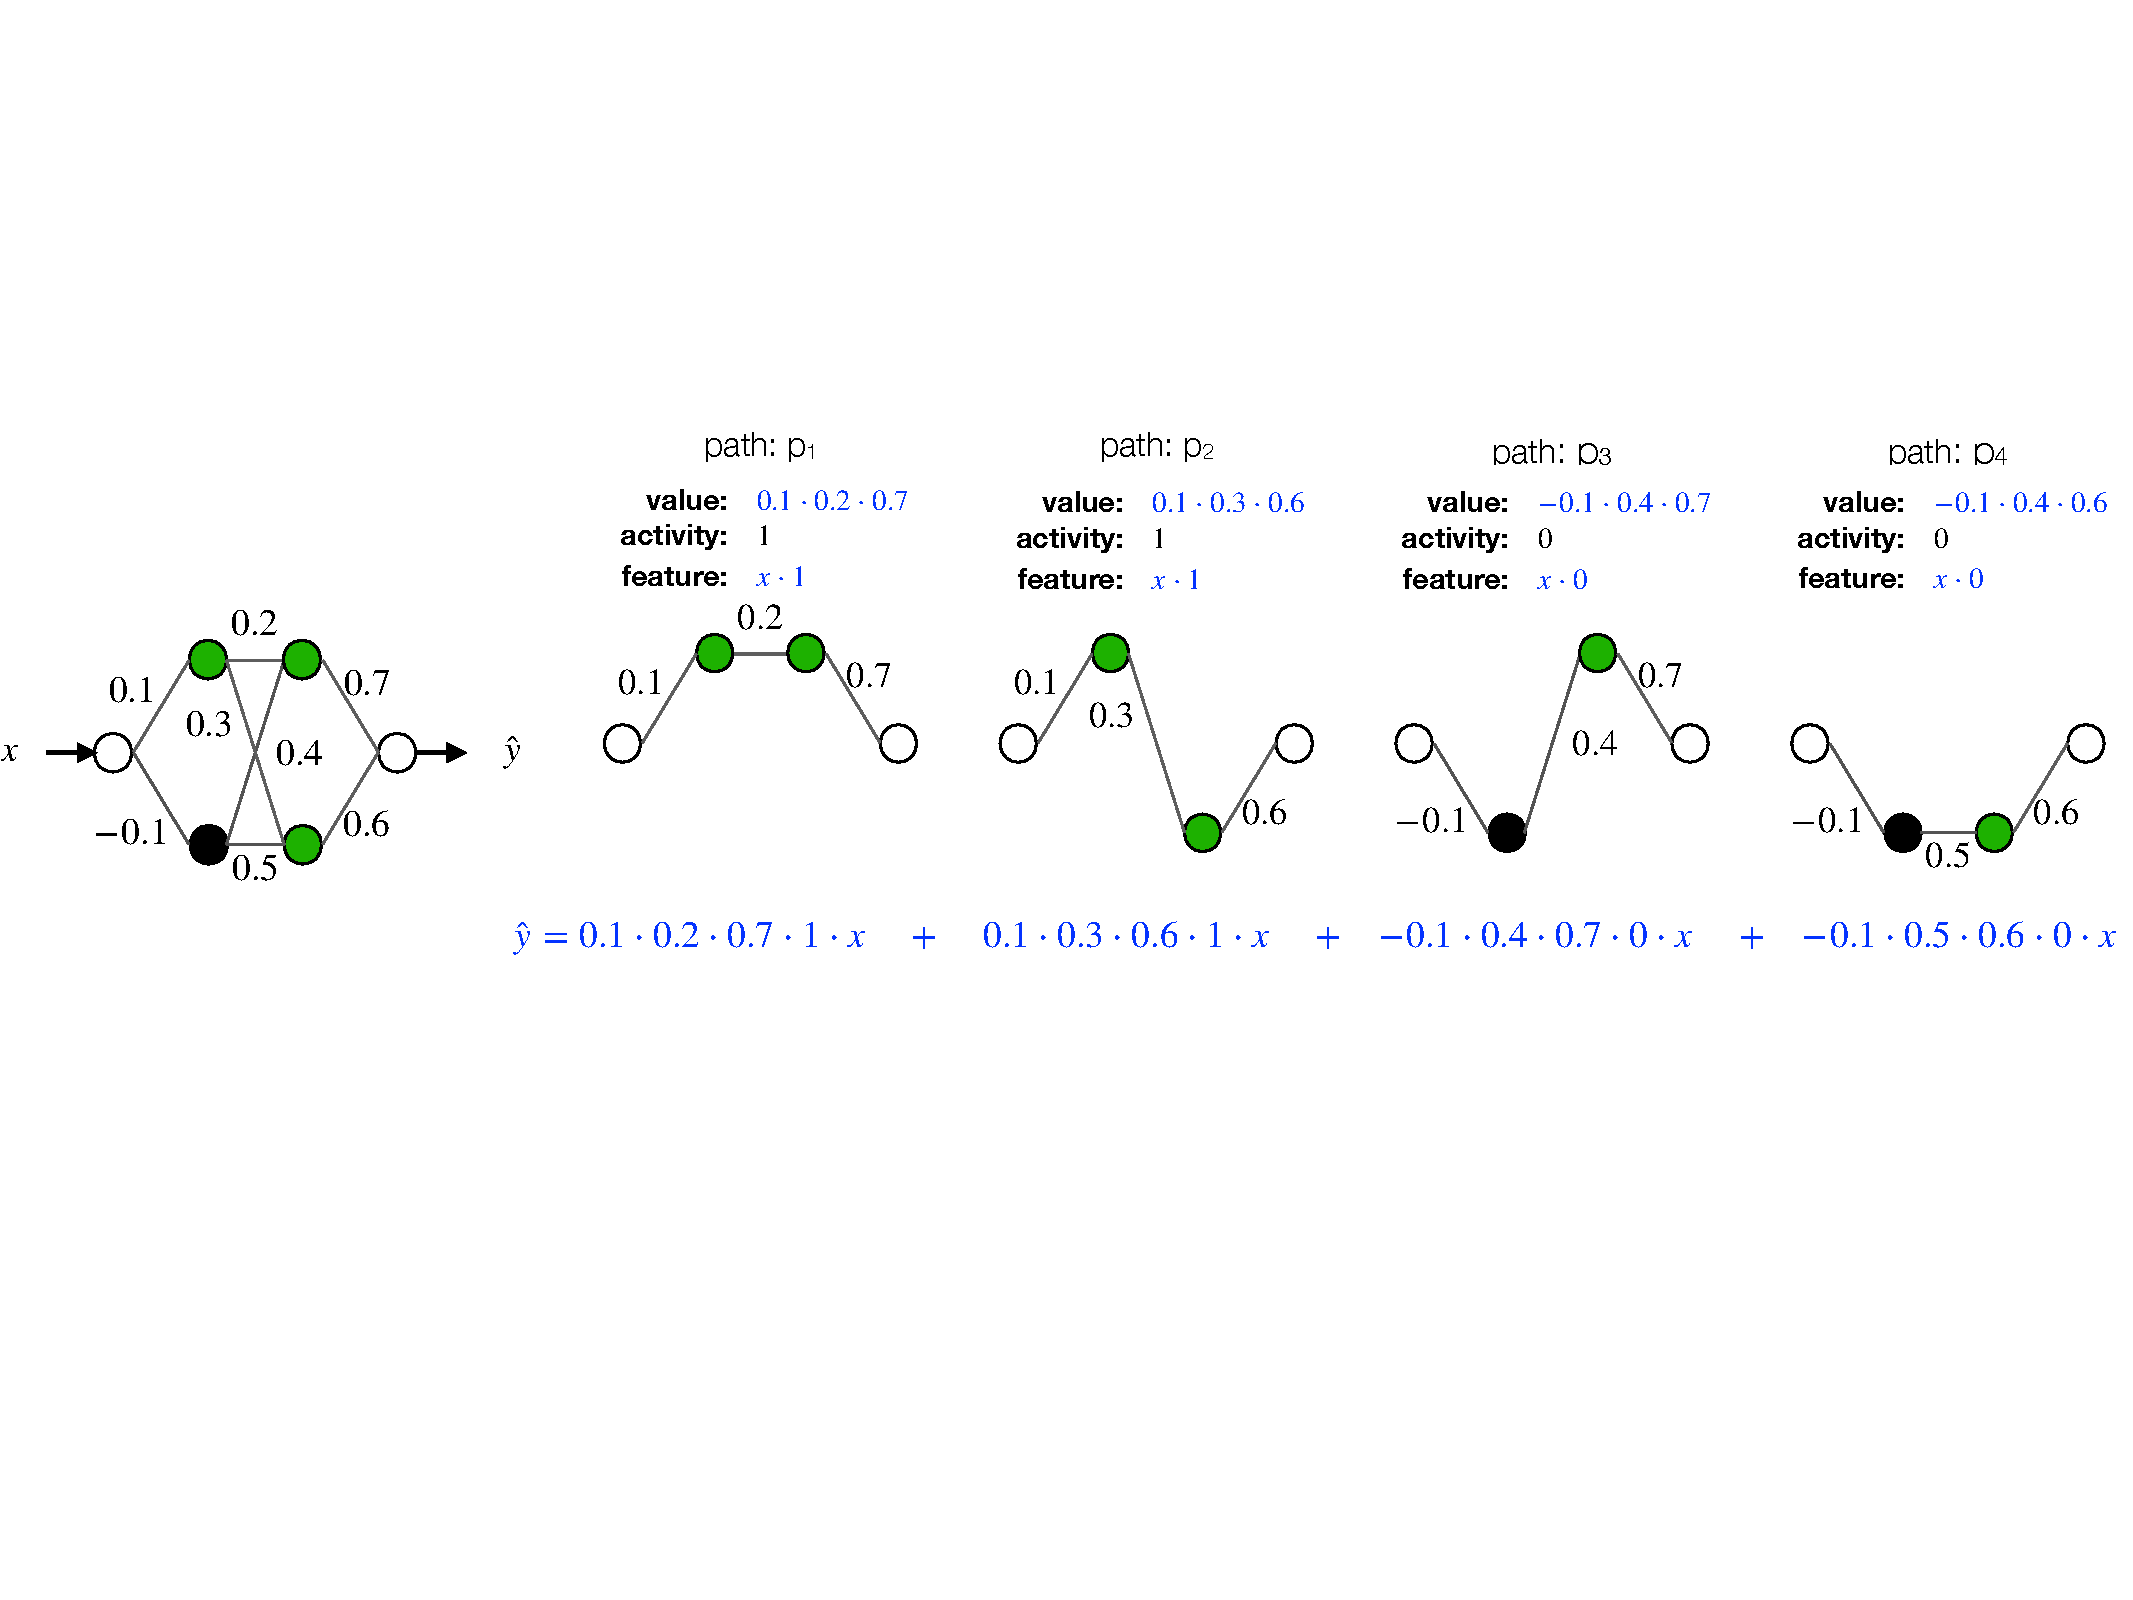
\includegraphics[scale=0.5]{figs/paths.pdf}
}
\caption{Illustration of \Cref{def:npf-npv} and \Cref{prop:npf-npv} in a  toy network with $2$ layers, $2$ gates per layer and $4$ paths. Paths $p_1$ and $p_2$ are `on' and paths $p_3$ and $p_4$ are `off'. The value, activity and feature of the individual paths are shown. $\hat{y}$ is the summation of the individual path contributions.}
\label{fig:paths}
\end{figure}

%\subsection{Overlap of Sub-Networks and Neural Path Kernel}
\begin{definition}[Overlap of active sub-networks]\label{def:overlap} 
The total number of `active' paths for both $x$ and $x'$ that pass through input node $i$ is defined to be:\\
{\centering{$\textbf{overlap}_{\Theta}(i,x,x') = \Lambda_{\Theta}(i,x,x') \eqdef \left|\{p\in[P]\colon  \Ifeat_0(p)=i, A_{\Theta}(x,p)= A_{\Theta}(x',p)=1\}\right|$}}
\end{definition}
%\subsection{NPK of FC-DNN: Product Kernel }
%\input{cnpkexample}
%\subsection{Neural Path Kernel : Similarity based on active sub-networks}
\begin{lemma}[Neural Path Kernel (NPK)]\label{lm:npk}
Let $D\in\R^{\din}$ be a vector of non-negative entries  and for $u,u'\in\R^{\din}$ , let $\ip{u,u'}_{D}=\sum_{i=1}^{\din}D(i)u(i)u'(i)$. Let $H_{\Theta}(x,x')\eqdef\langle\phi_{x,\Theta},\phi_{x',\Theta} \rangle$ be the neural path kernel (NPK). Then  
\begin{align*} 
\text{NPK}_{\Theta}(x,x')= H_{\Theta}(x,x')=\ip{x,x'}_{\Lambda_{\Theta}(\cdot,x,x')} 
\end{align*}
\end{lemma}
\textbf{Remark.} In the case of fully connected networks, $\textbf{overlap}_{\Theta}(i,x,x')$ is equal for all $i\in[\din]$, and hence $\text{NPK}_{\Theta}(x,x')=\ip{x,x'}\cdot\textbf{overlap}_{\Theta}(x,x')$.

\subsection{Deep Gated Network : Decoupling Gates (NPF) and Weights (NPV) }\label{sec:dgn}
\begin{comment}
\begin{wrapfigure}{r}{0.2\textwidth}
\centering
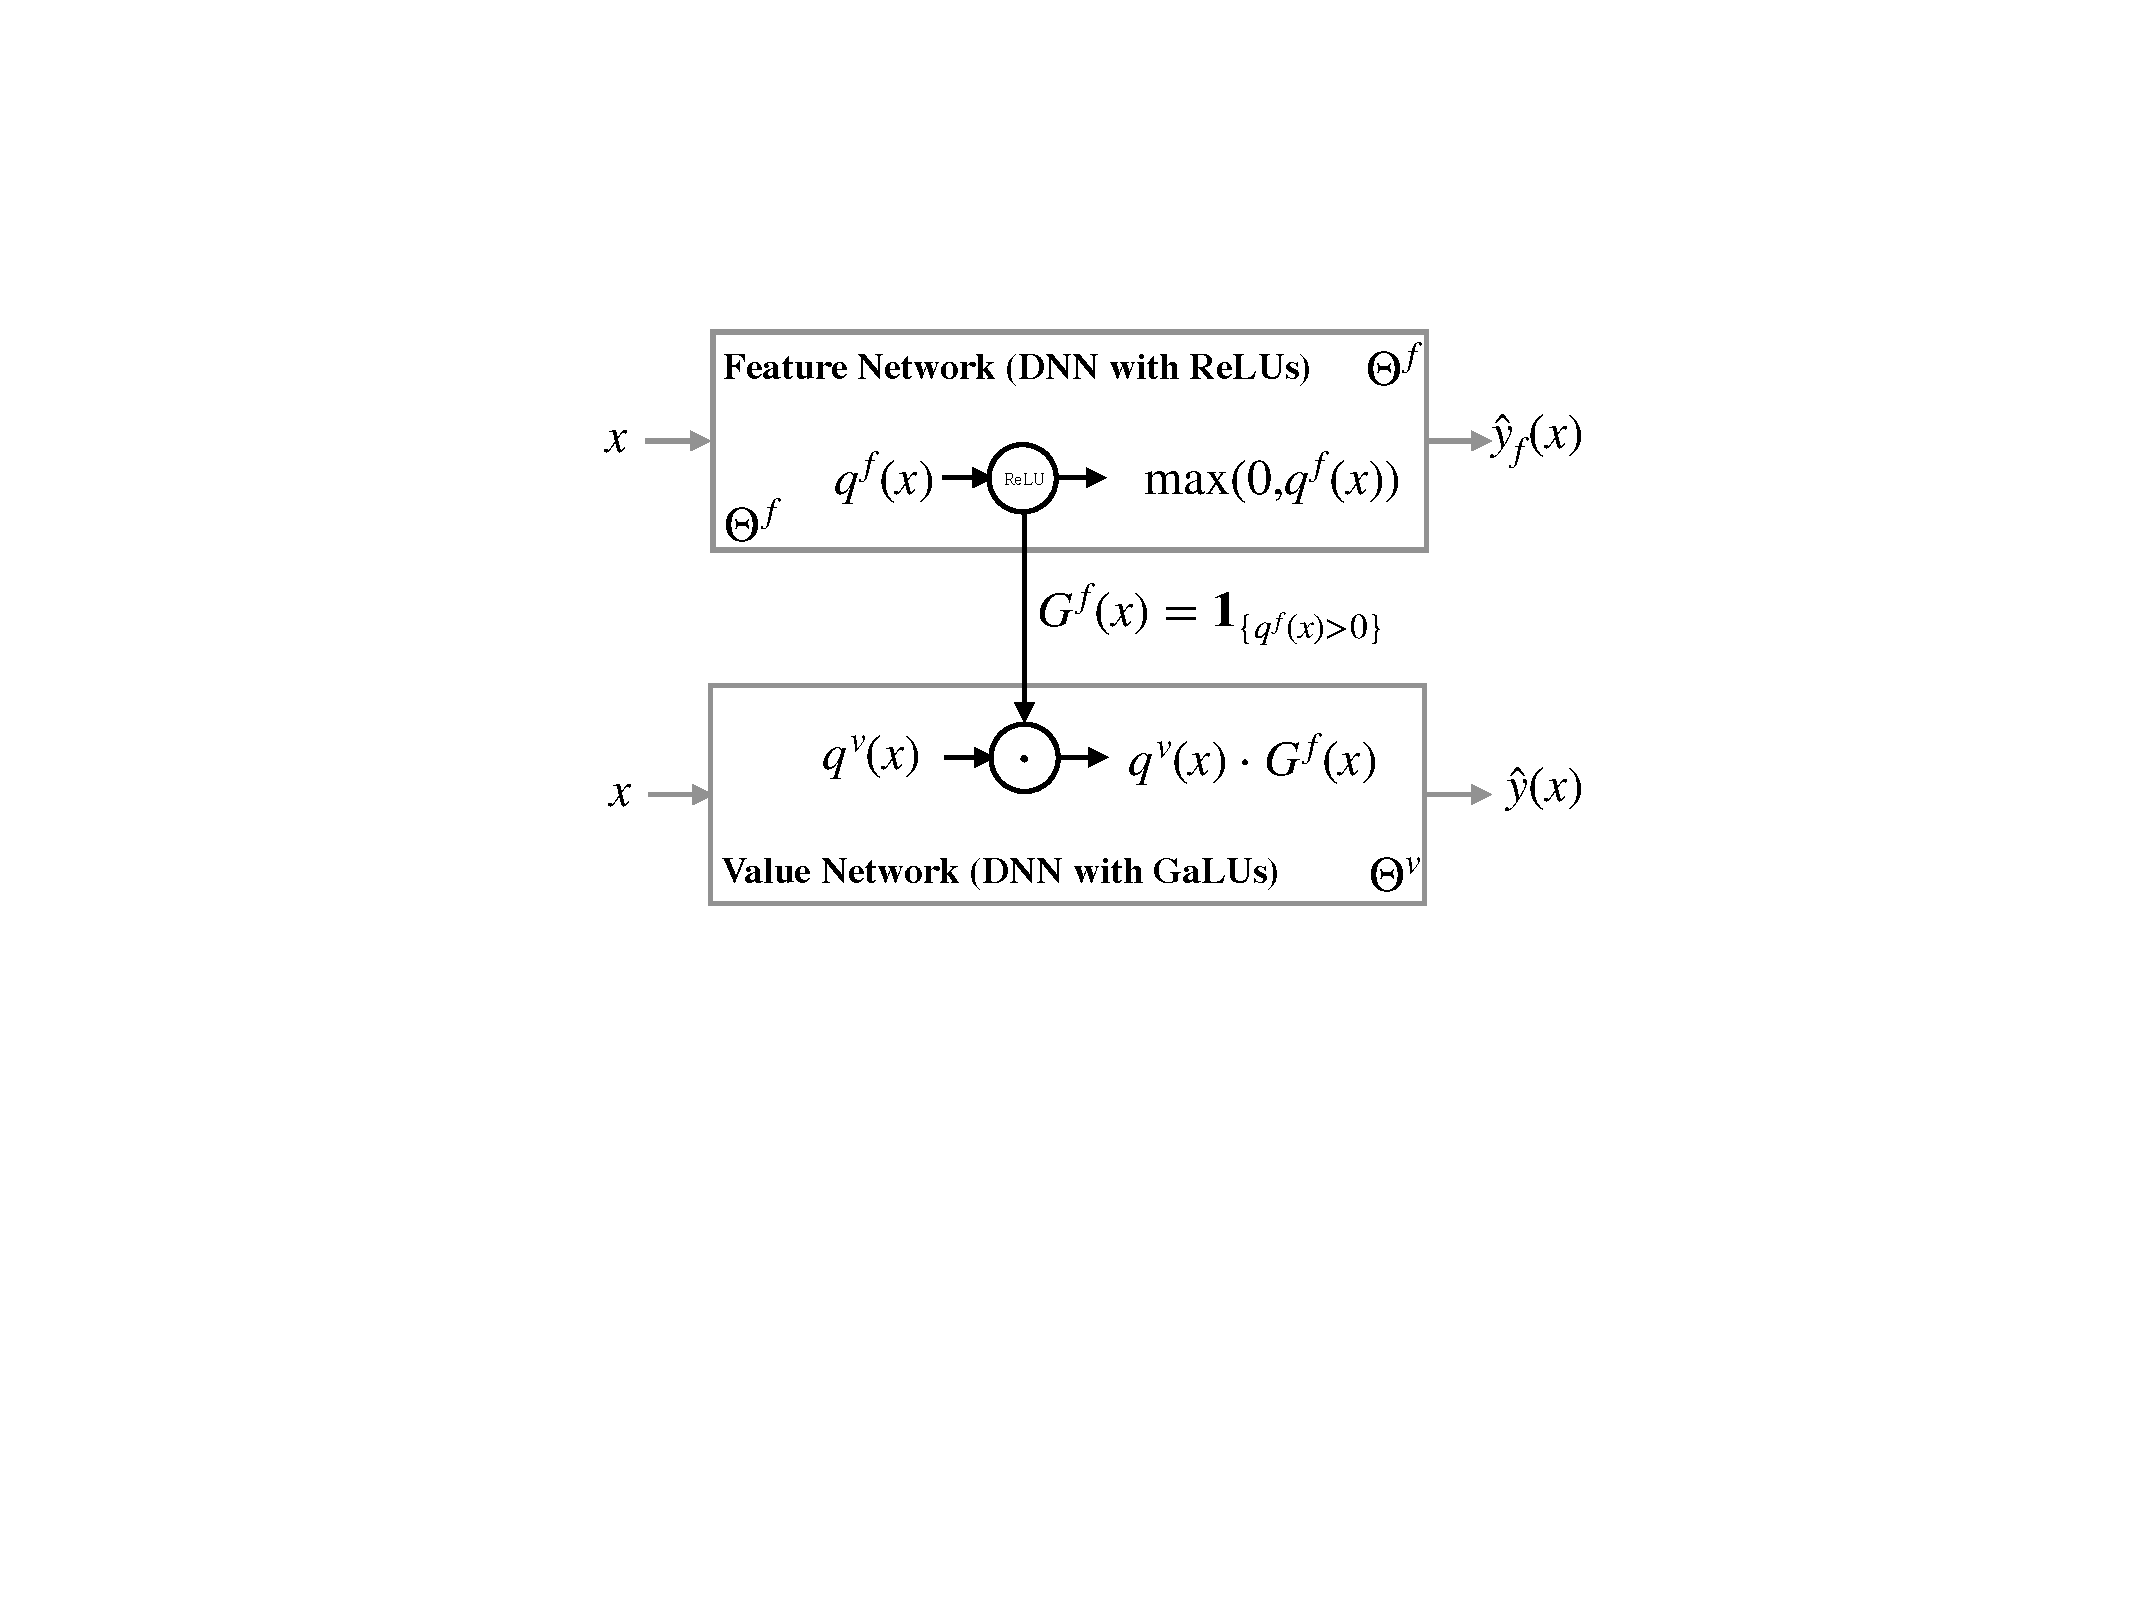
\includegraphics[scale=0.1]{figs/dgn-nips.pdf}
\caption{DGN}
\label{fig:dgn}
\end{wrapfigure}
\end{comment}

Since $\hat{y}_{\Theta}(x)=\ip{\phi_{x,\Theta},v_{\Theta}}$, during training, as $\Theta$ is learnt, both the NPFs and NPV are also learnt. To understand their roles better, $\phi_{x,\Theta}$ and $v_{\Theta}$ have to be separated.  This is achieved by the deep gated network (DGN) setup (see \Cref{fig:dgn}), which has two networks of \emph{identical architecture} namely the \emph{feature network} ($\Tf\in\R^{d^{\text{f}}_{\text{net}}}$) which holds the NPFs (i.e., the gating information) and the \emph{value network} ($\Tv\in\R^{d^{\text{v}}_{\text{net}}}$) which holds the NPV.  The combined parameterisation is denoted by $\Theta^{\text{DGN}}=(\Tf,\Tv)\in \R^{d^{\text{f}}_{\text{net}}+d^{\text{v}}_{\text{net}}}$.  The feature network is a DNN with ReLUs and the value network is a DNN with \emph{Gated Linear Units (GaLUs)} (terminology used in [\citenum{sss}]) whose output is the product of its pre-activation input $q^{\text{v}}(x)$and the external gating signal $G^{\text{f}}(x)$ (see \Cref{fig:dgn}). In \Cref{fig:dgn}, the main output of the DGN is $\hat{y}_{\text{DGN}}(x)$, while the other output $\hat{y}_{\text{f}}(x)$ is used to \emph{pre-train} the gates (see \Cref{sec:exp}).

\begin{figure}[h]
\begin{minipage}{0.38\columnwidth}
\resizebox{0.8\columnwidth}{!}{
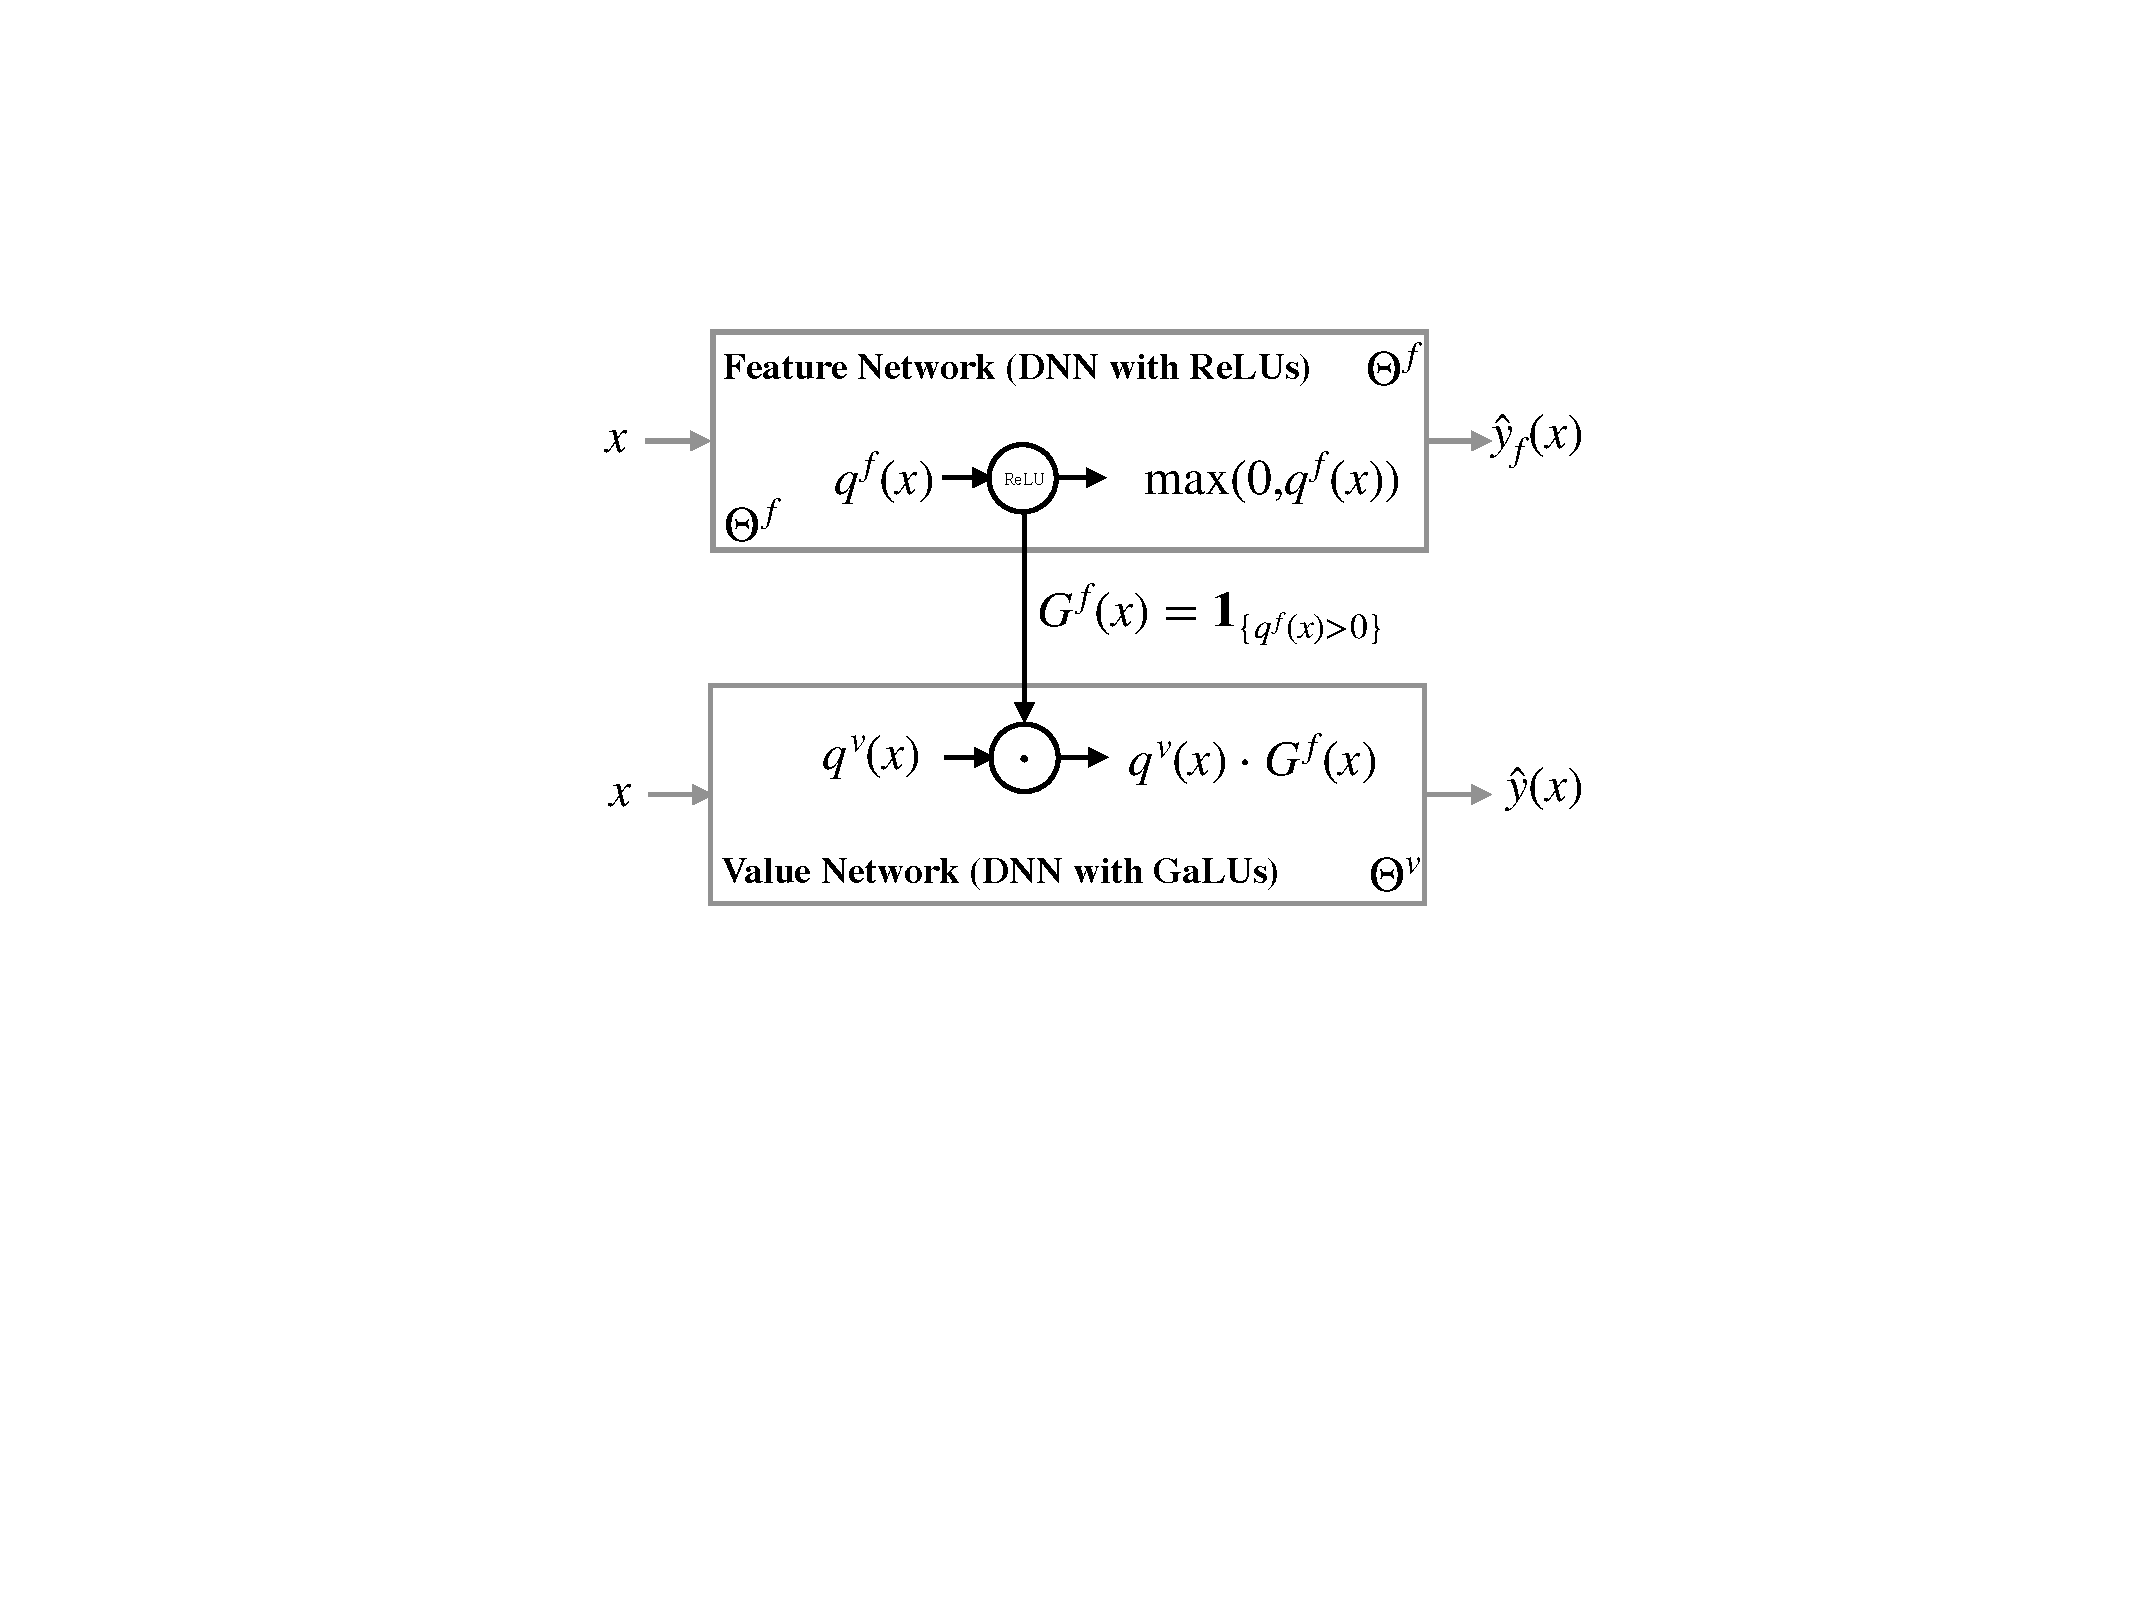
\includegraphics[scale=0.4]{figs/dgn-nips.pdf}
}
\caption{\small{Shows a DGN and interaction between two corresponding units, one in the feature and other in value network.}}
\label{fig:dgn}
\end{minipage}
\hfill
%\begin{flushright}
\begin{minipage}{0.55\columnwidth}
\begin{proposition}[{[\citenum{npk}]}]\label{prop:ntks} Let $\kv_{\Tdgn}(x,x')=\ip{ \nabla_{\Tv}\hat{y}_{\text{DGN}}(x), \nabla_{\Tv}\hat{y}_{\text{DGN}}(x')}$, and  $\kf_{\Tdgn}(x,x')=\ip{ \nabla_{\Tf}\hat{y}_{\text{DGN}}(x), \nabla_{\Tf}\hat{y}_{\text{DGN}}(x') }$ and $K_{\Tdgn}(x,x')$ be the NTK of the DGN. Then 
\begin{align*}
K_{\Tdgn}(x,x')=\kv_{\Tdgn}(x,x')+\kf_{\Tdgn}(x,x')
\end{align*}
\textbf{Remarks.} $\nabla_{\Tf}\hat{y}_{\text{DGN}}(x)$ flows via the feature network and $\nabla_{\Tv}\hat{y}_{\text{DGN}}(x)$ via the value network. Correspondingly there are two NTKs, i.e., $\kf$ and $\kv$. If the gates are fixed then, $\nabla_{\Tf}\hat{y}_{\text{DGN}}(x)=\mathbf{0}$ and $\kf_{\Tdgn}(x,x')=0$. 
\end{proposition}
%The deep gated network (DGN) setup (see \Cref{fig:dgn}), which has two networks namely the \emph{feature network} parameterised by $\Tf\in\R^{d^{\text{f}}_{\text{net}}}$ which holds the NPFs (i.e., the gating information) and a \emph{value network} parameterised by $\Tv\in\R^{d^{\text{v}}_{\text{net}}}$ which holds the NPV.  The combined parameterisation is denoted by $\Theta^{\text{DGN}}=(\Tf,\Tv)\in \R^{d^{\text{f}}_{\text{net}}+d^{\text{v}}_{\text{net}}}$.  
\end{minipage}
%\end{flushright}
\begin{comment}
\begin{minipage}{0.73\columnwidth}
\resizebox{\columnwidth}{!}{
\begin{tabular}{|ll|}\hline
Feature Network & Value Network\\
$z_{x,\Theta}(0)=x$& $z_{x,\Theta}(0)=x$ \\
$q_{x,\Theta}(i,l)=\sum_{j} \Theta(i,j,l)\cdot z_{x,\Theta}(j,l-1)$& $q_{x,\Theta}(i,l)=\sum_{j} \Theta(i,j,l)\cdot z_{x,\Theta}(j,l-1)$\\
$G_{x,\Theta}(i,l)=\mathbbm{1}_{\{q_{x,\Theta}(i,l)>0\}}$& $G_{x,\Theta}(i,l)=\mathbbm{1}_{\{q_{x,\Theta}(i,l)>0\}}$\\
$z_{x,\Theta}(i,l)=q_{x,\Theta}(i,l)\cdot G_{x,\Theta}(i,l)$ & $z_{x,\Theta}(i,l)=q_{x,\Theta}(i,l)\cdot G_{x,\Theta}(i,l)$ \\
 $\hat{y}_{\Theta}(x)=\sum_{j\in[w]} \Theta(1,j,d-1)\cdot z_{x,\Theta}(j,d-1)$ & $\hat{y}_{\Theta}(x)=\sum_{j\in[w]} \Theta(1,j,d-1)\cdot z_{x,\Theta}(j,d-1)$\\\hline
\end{tabular}
}
\end{minipage}
\end{comment}
\end{figure}

\begin{comment}
\subsection{NTK $\propto$ NPK}
\begin{assumption}\label{assmp:main}
(i) $\Tv_0$ is statistically independent of $\Tf_0$ (ii) $\Tv_0$ are i.i.d symmetric Bernoulli over $\{-{\sigma},+{\sigma}\}$. 
\end{assumption}

\begin{theorem}\label{th:main} Let $\sigma=\frac{\cscale}{\sqrt{w}}$. Under \Cref{assmp:main}, a $w\ra\infty$, for FC-DGN we have: 
\begin{align*}
\kv_{\Tdgn_0}(x,x') &\ra d\cdot \sigma^{d-1}\cdot H_{\Tf_0}(x,x')= d\cdot \sigma^{d-1}\cdot \ip{x,x'}_{\Lambda_{\Tf_0}(\cdot,x,x')}  \\
\end{align*}
\end{theorem}
\begin{figure}[h]
\begin{minipage}{0.49\columnwidth}
\centering
\resizebox{\columnwidth}{!}{
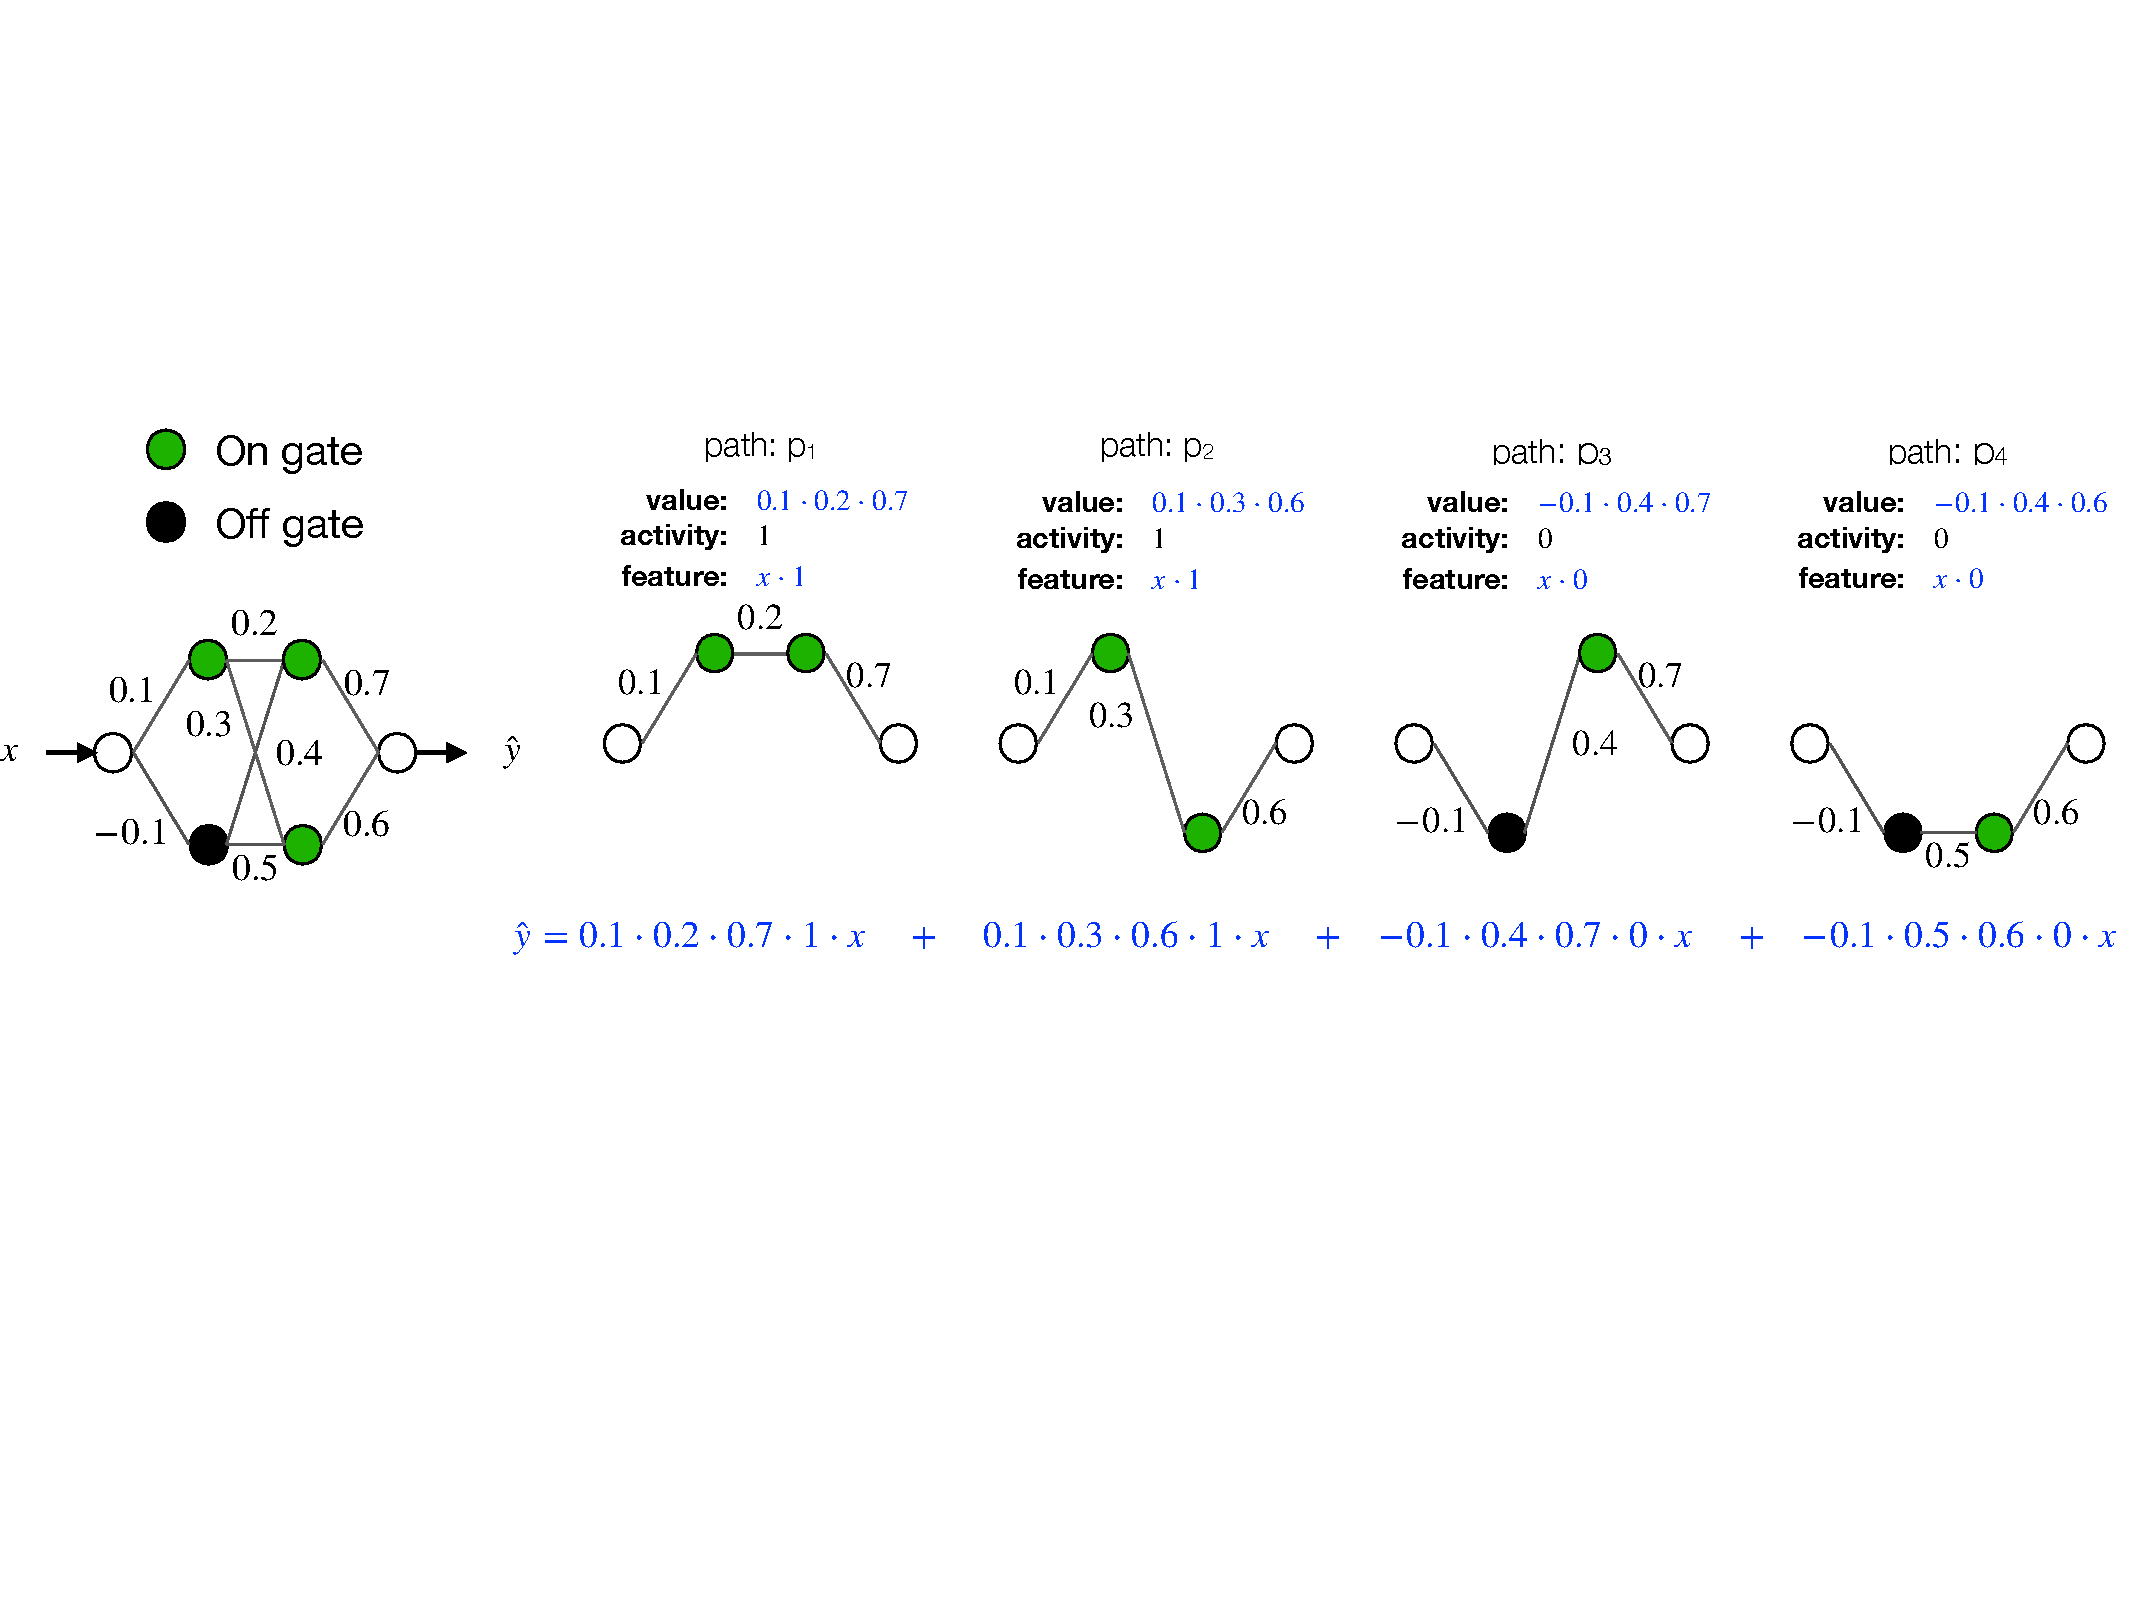
\includegraphics[scale=0.5]{figs/overlap.pdf}
}
\end{minipage}
\begin{minipage}{0.49\columnwidth}
\resizebox{\columnwidth}{!}{
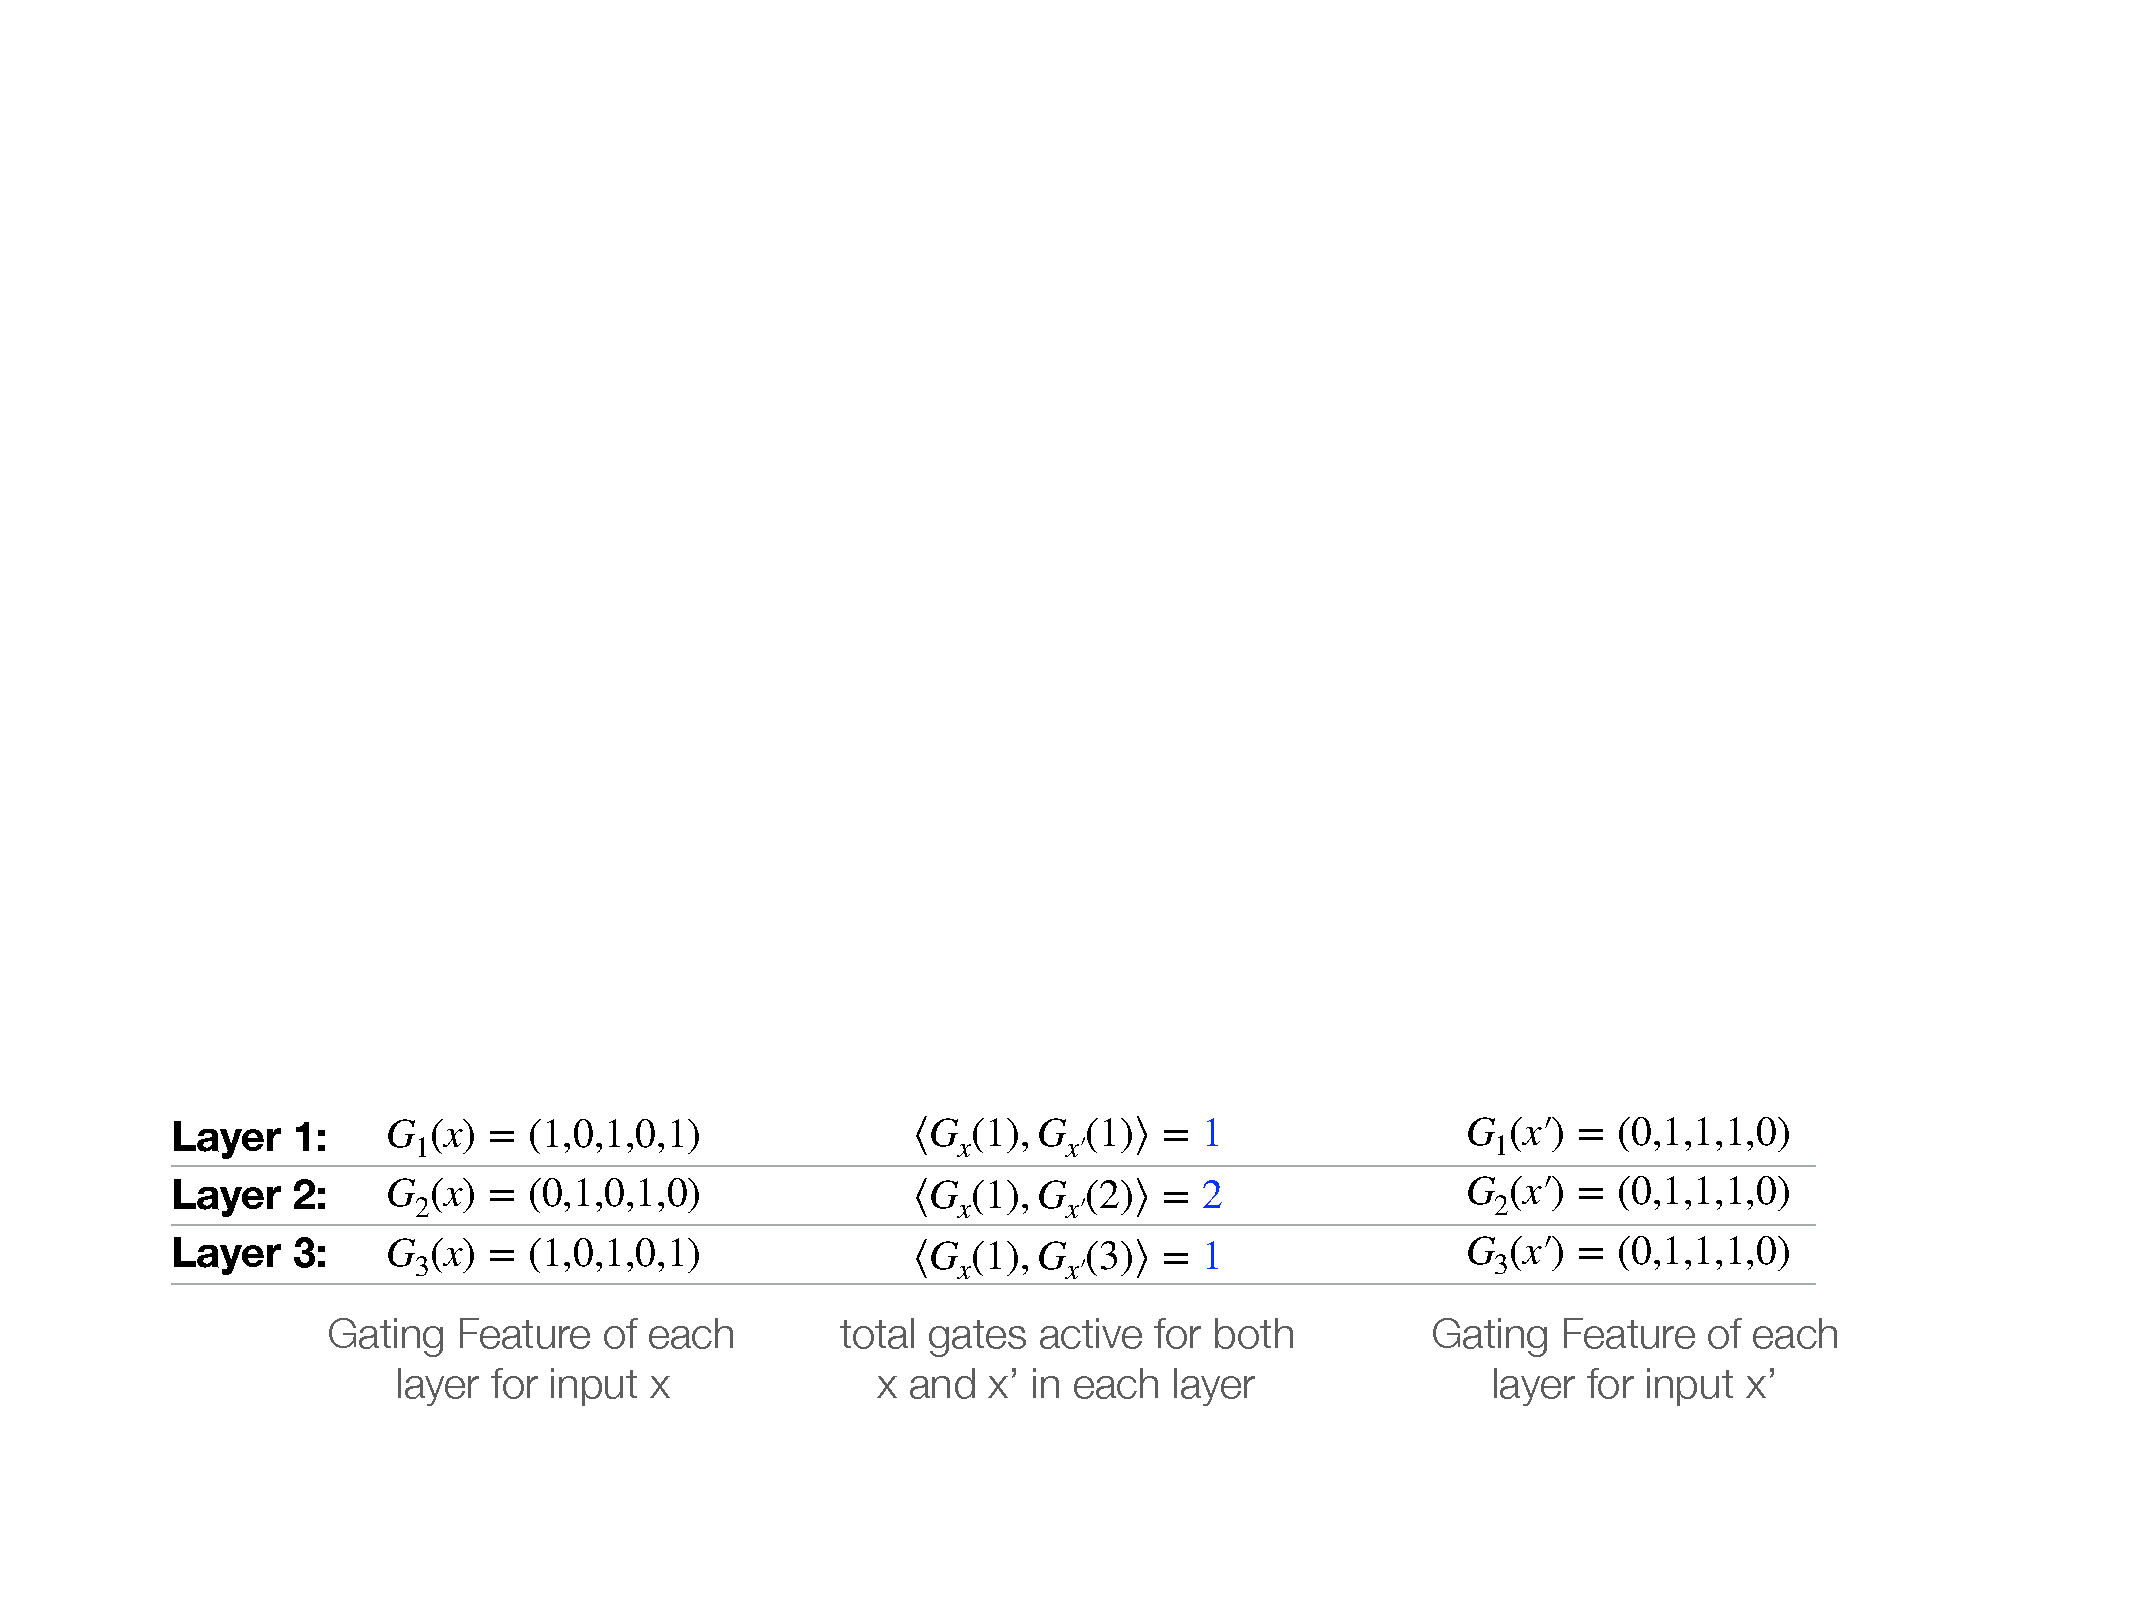
\includegraphics[scale=0.5]{figs/gating-features.pdf}
}
\end{minipage}
\caption{Shows a toy illustration of active sub-networks for two inputs $x$ and $x'$ and the common overlapping sub-network. The total number of active paths from any input node $i$, $\Lambda(i,x,')=\Pi_{i=1}^{3} \ip{G_l(x),G_l(x'}=1\cdot 2\cdot 1 =2$.}
\label{fig:overlap}
\end{figure}
\end{comment}
\section{Theoretical Result}\label{sec:fc}
Our goal is to characterise `what is learnt in the gates of a DNN with ReLUs'. To this end, we use the DGN setup where the gates and weights are separate. Specifically, the DNN with ReLUs whose gates we want to examine is the feature network in the DGN. We then measure the information in the gates by keeping the gates fixed and training the value network and measuring the test performance of the value network. It was shown in [\citenum{npk}] that if the gates are fixed  (i.e., with reference to \Cref{prop:ntks}, $\kf=0$), for fully connected DGN, the NTK simplifies as $\text{NTK}(x,x')\propto \text{NPK}(x,x') = \ip{x,x'}\cdot {\bf{overlap}}(x,x')$. In this section, we state three results, where in \Cref{th:main} we `re-write' Theorem~$5.1$ in [\citenum{npk}] to explicitises the role of gates, width and depth, to yield a simple product of kernels expression (unknown in prior works).  \Cref{th:mainconv} covers the case of convolutions with pooling and \Cref{th:mainres} covers the case residual networks with skip connections.

\textbf{Note 1.} The gates of the DGN can also be tuned in which case $\kf\neq \mathbf{0}$, and we reserve the study of $\kf$ for future. The results are for infinite width networks and at randomised initialisation. We use these insights as an indicator of what we can expect when we experiment with finite width networks. 

We begin with an assumption that states that the value network weights have to be statistically independent of the feature network weights at initialisation. %With reference to \Cref{prop:ntks}, since the gates fixed, it follows that $\kf=\mathbf{0}$ and we will characterise only $\kv$ which corresponds to the value network. Here, the DGN is used to study the gates of a \emph{untrained/(partially or fully) trained} DNN with ReLUs. We wish to point that the gates of the DGN can also be tuned in which case $\kf\neq \mathbf{0}$, and we reserve the study of $\kf$ for future. We now state an assumption on the value network 

%In this section, we state three results (\Cref{th:main,th:mainconv,th:mainres}) that characterise `what is learnt in the gates of a DNN with ReLUs'.  To this end, we use the DGN setup where the gates and weights are separate. Specifically, the DNN with ReLUs whose gates we want to examine becomes the feature network in the DGN. If we keep the feature network weights fixed, the gates are automatically fixed. We then characterise the information in the gates by training the value network and measuring the test performance of the value network. With reference to \Cref{prop:ntks}, since the gates fixed, it follows that $\kf=\mathbf{0}$ and we will characterise only $\kv$ which corresponds to the value network. Here, the DGN is used to study the gates of a \emph{untrained/(partially or fully) trained} DNN with ReLUs. 

\begin{assumption}\label{assmp:main}
$\Tv_0\stackrel{\text{i.i.d}}\sim\text{Bernoulli}(\frac12)$ over $\{-{\sigma},+{\sigma}\}$ and statistically independent of $\Tf_0$.
\end{assumption}
We point out that this statistical decoupling of weights and gates in \Cref{assmp:main} is unrealisable in a DNN with ReLU, however, this assumption can be trivially realised in a DGN.
\begin{theorem}[Product of Kernels Theorem]\label{th:main} Under \Cref{assmp:main}  ($\sigma=\frac{\cscale}{\sqrt{w}}$) for FC-DGN : 
\begin{align*}
\kv_{\Tdgn_0}(x,x') \ra d\cdot \cscale^{d-1} \cdot \left(\ip{ x,x'} \cdot \Pi_{l=1}^{d-1} \frac{\ip{G_l(x),G_l(x')}}w\right), \quad\text{as}\,\, w\ra\infty 
\end{align*}
\end{theorem} 
\textbf{Key Insight.} Here $\frac{\ip{G_l(x),G_l(x')}}w$ are the \emph{base kernels} measuring the \emph{\textbf{correlation of the gates}}. We show experimentally that the correlation of gates is essentially  `what is learnt in a DNN with ReLUs'.
%and $\Pi_{l=1}^{d-1} \frac{\ip{G_l(x),G_l(x')}}w$ is a product of these base kernels and hence the name `Product of Kernels Theorem'.  The base kernels are essentially measuring which we show via  We now list the roles of the two networks, weights, depth and width.

\textbf{Feature Network.} The role of this network is to process the input layer-by-layer and produce the $w$-dimensional gating features $G_l(\cdot)$. Each layer comprises of `$w$' ReLUs, and a given ReLU (i.e., gate) is `on' if the input to that layer lies on the positive half-space of hyperplane of given by the incoming weights of that ReLU. Thus the gates of a given layer are based on the angle between the input to that layer and the various hyperplanes given by the weights of that layer. Prior experiments in [\citenum{npk}] and the experiments in this paper show that the feature network, i.e., the gates hold most information, which in turn means that weights of the feature network are key.

\textbf{Value Network}. The value network implements the product of kernels by laying out the gates as masks depth-wise, and connecting them in the structure of a DNN. Note that depth-wise layout plays an important role here: for instance, if we were to concatenate the gating features as $\varphi(x)=(G_l(x),l=1,\ldots,d-1)\in\{0,1\}^{(d-1)w}$, it would have only resulted in the kernel $\ip{\varphi(x),\varphi(x')}=\sum_{l=1}^{d-1}{\ip{G_l(x),G_l(x')}}$, i.e., a \emph{sum  (not product)} of kernels. Prior experiments in [\citenum{npk}] and the experiments in this paper show that the value network can be reset and re-trained without loss of performance, which in turn means that weights of the value network are not that important.

\textbf{Note.} The above insights from \Cref{th:main} carry over to the case of DNN with ReLUs by thinking that the roles of value and feature network are performed by a single network.

\textbf{Convolutions with pooling.} Let the circular rotation of vector $x\in\R^{\din}$ by `$r$' co-ordinates be defined as $rot(x,r)(i)=x(i+ r)$, if $i+r \leq \din$ and $rot(x,r)(i)=x(i+ r-din)$ if $i+r > \din$. Using circular convolutions with pooling results in a rotationally invariant kernel \Cref{th:mainconv}. The architecture and the notations for the network with convolutions is presented in the Appendix.
\begin{comment}
 We extend the dual view to neural network with $\dc$ convolutional layers ($l=1,\ldots,\dc$), followed by a \emph{global-average/max-pooling} layer ($l=\dc+1$) and $\dfc$ ($l=\dc+2,\ldots,\dc+\dfc+1$) fully connected  layers (see Appendix for notation). The convolutional window size is $\wconv<\din$, the number of filters per convolutional layer as well as the width of the fully connected layers is $w$. The main steps are (i) treating pooling layers like gates/masks, (ii) bundling together the paths that share the same path value (due to weight sharing in convolutions) and (iii) re-defining the NPF and NPV for these bundles. The important consequence of weight sharing (due to convolutions and pooling) is that the NPK becomes rotationally invariant resulting in \Cref{th:mainconv}.
\end{comment}
\begin{theorem}[Rotationally Invariant Kernel Theorem]\label{th:mainconv} Under \Cref{assmp:main}, for  a suitable $\bcnn$:
\begin{align*}
&\kv_{\Tdgn_0}&\ra&\quad \frac{\bcnn}{{\din}^2} \cdot \sum_{r=0}^{\din-1} \ip{x,rot(x',r)}_{\Lambda(\cdot, x,rot(x',r))},\,\, \text{as}\,\,  w\ra\infty\,\text{(for global-average-pooling)}, \\
&\kv_{\Tdgn_0}&\ra& \quad{\bcnn} \cdot \sum_{r=0}^{\din-1} \ip{x,rot(x',r)}_{\Lambda(\cdot, x,rot(x',r))},\,\, \text{as}\,\,  w\ra\infty\,\text{(for global-max-pooling)}
\end{align*}
\end{theorem}
\textbf{Remark.}  $\Lambda(i,x,x')$ counts the number of paths starting from input node $i$ that are active for both $x$ and $x'$. The summation can be expanded as $\sum_{r=0}^{\din-1} \ip{x,rot(x',r)}_{\Lambda(\cdot, x,rot(x',r))}=\sum_{r=0}^{\din-1} \left(\sum_{i=1}^{\din} x(i) rot(x',r)(i)\Lambda(i,x,x')\right)$, where the inner $\Sigma$ is the inner product between $x$ and $rot(x',r)$ weighted by $\Lambda$ and the outer $\Sigma$ covers all possible rotations.

\textbf{Residual Networks with Skip connections.} We consider a ResNet with `$(b+2)$' blocks and `$b$' skip connections between the blocks (left of \Cref{fig:resnet}). Each block is a fully connected (FC) DNN of depth `$\dblock$' and width `$w$'. There are combinatorially many sub-FC-DNNs within this ResNet (see \Cref{def:subfcdnn} and right of \Cref{fig:resnet}).
\FloatBarrier
\begin{figure}[h]
\begin{minipage}{0.5\columnwidth}
\resizebox{\columnwidth}{!}{
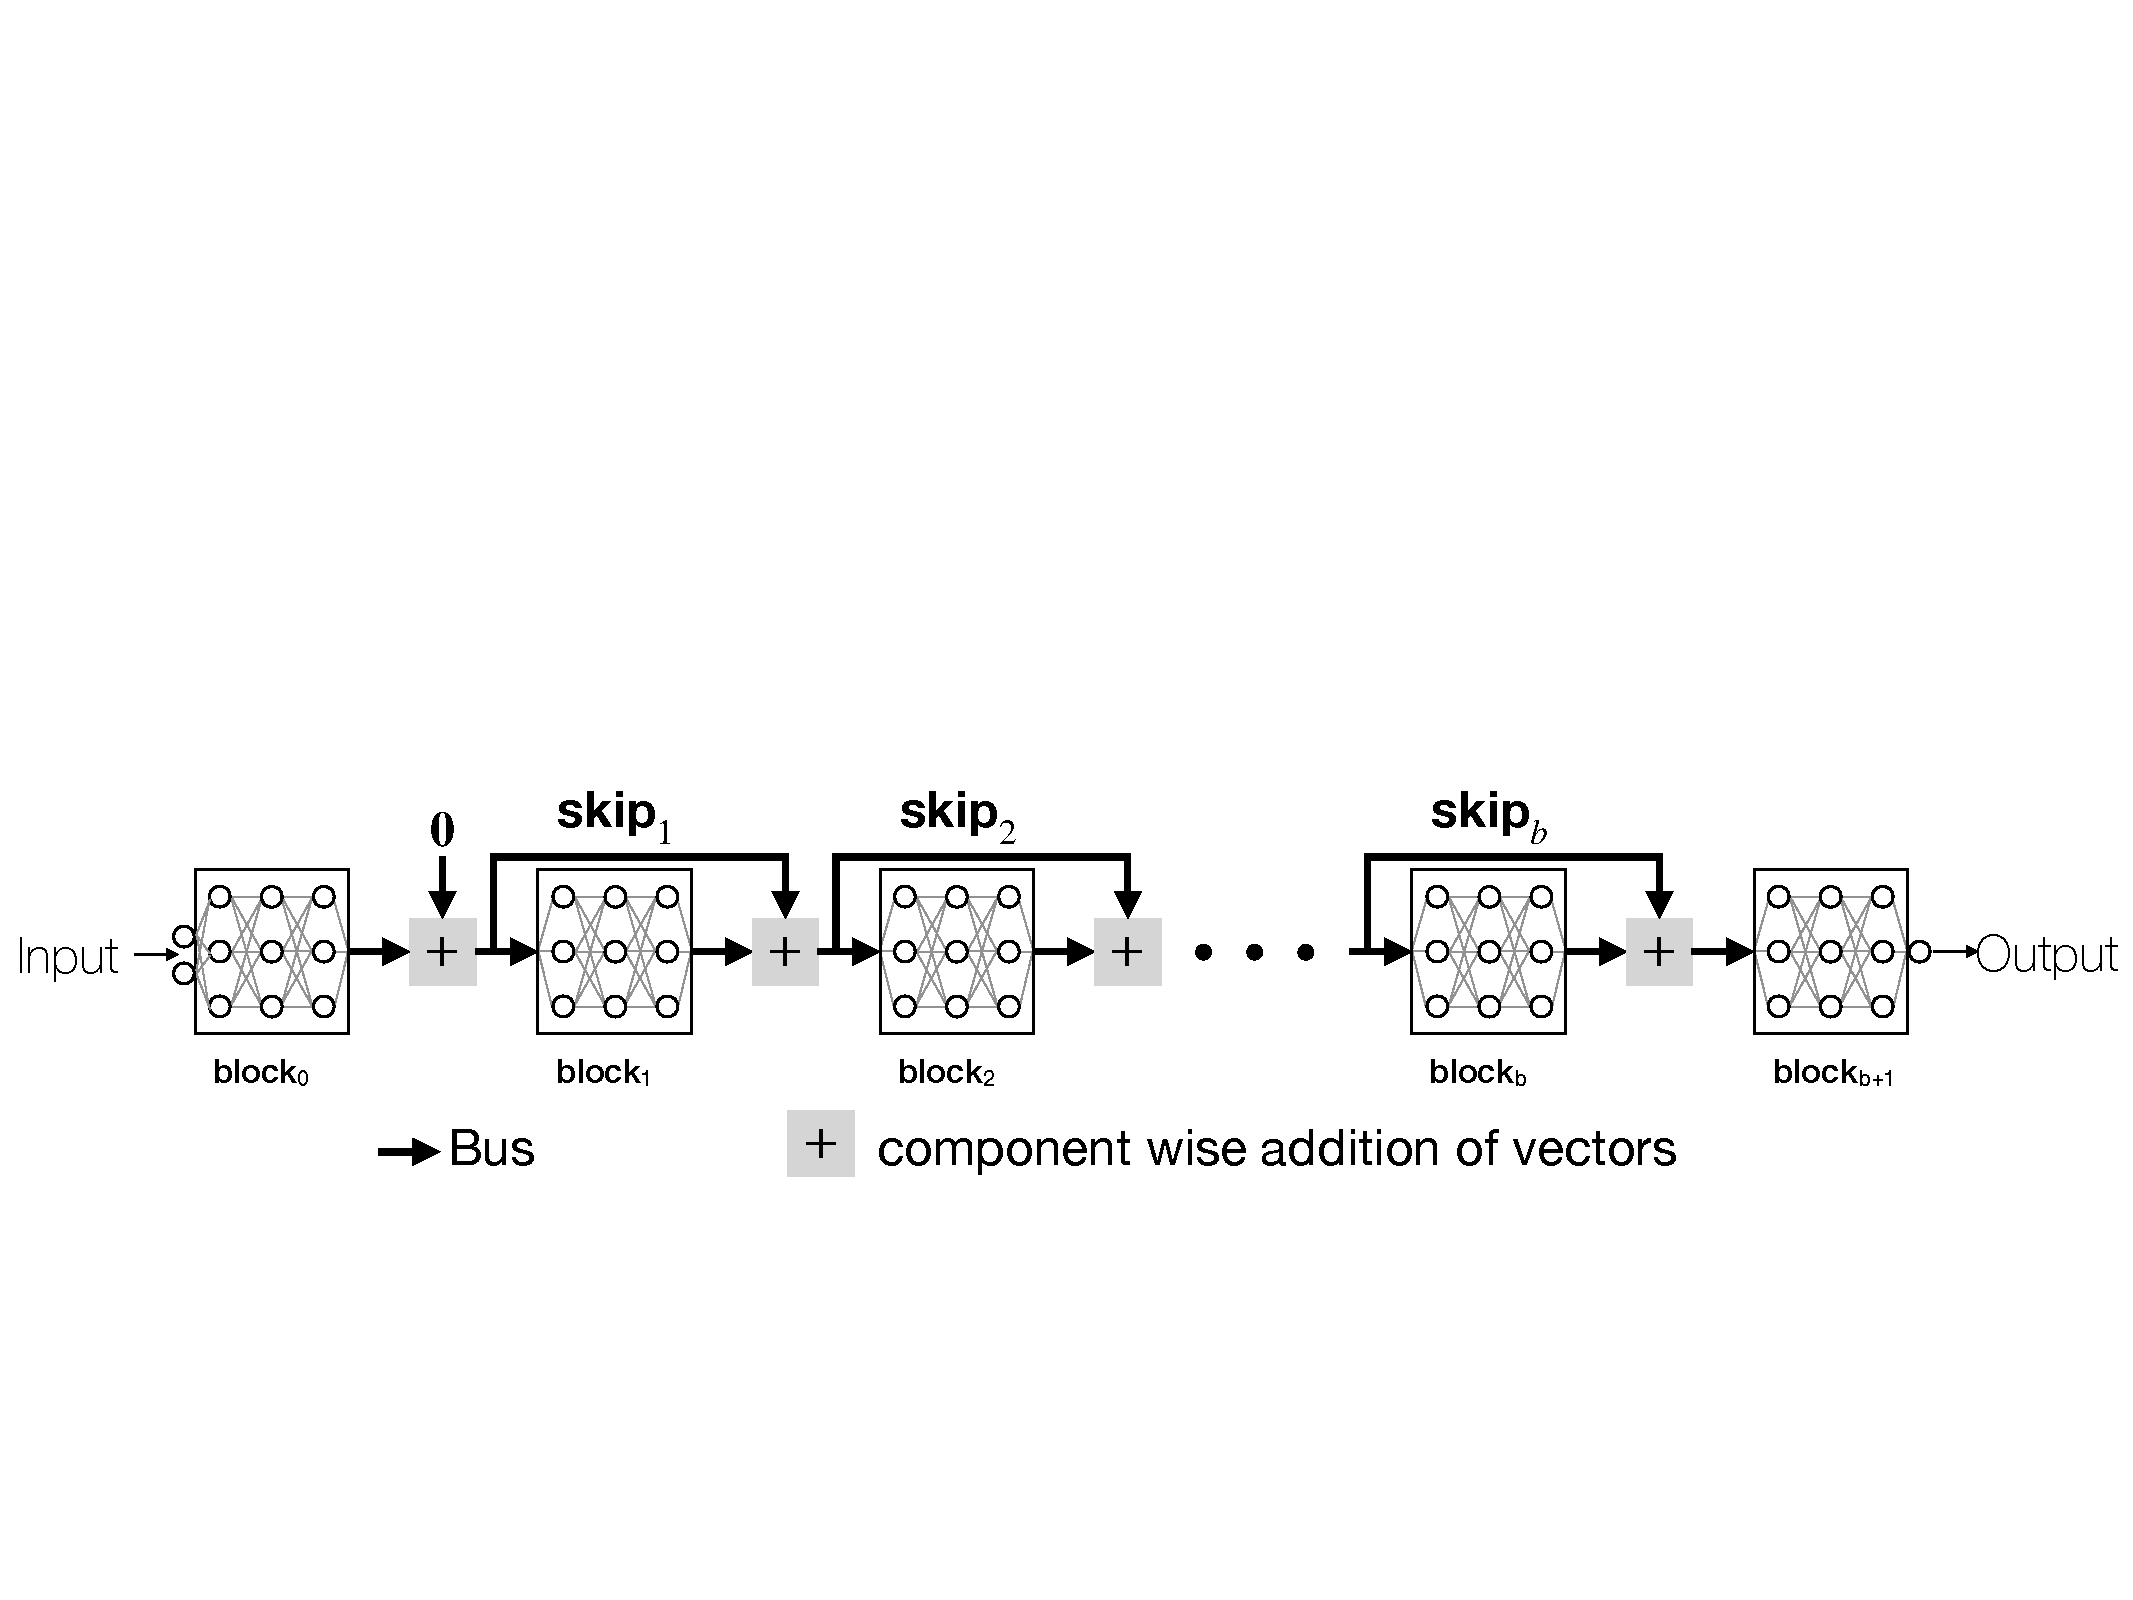
\includegraphics[scale=0.5]{figs/resnet.pdf}
}
\end{minipage}
\begin{minipage}{0.5\columnwidth}
\resizebox{\columnwidth}{!}{
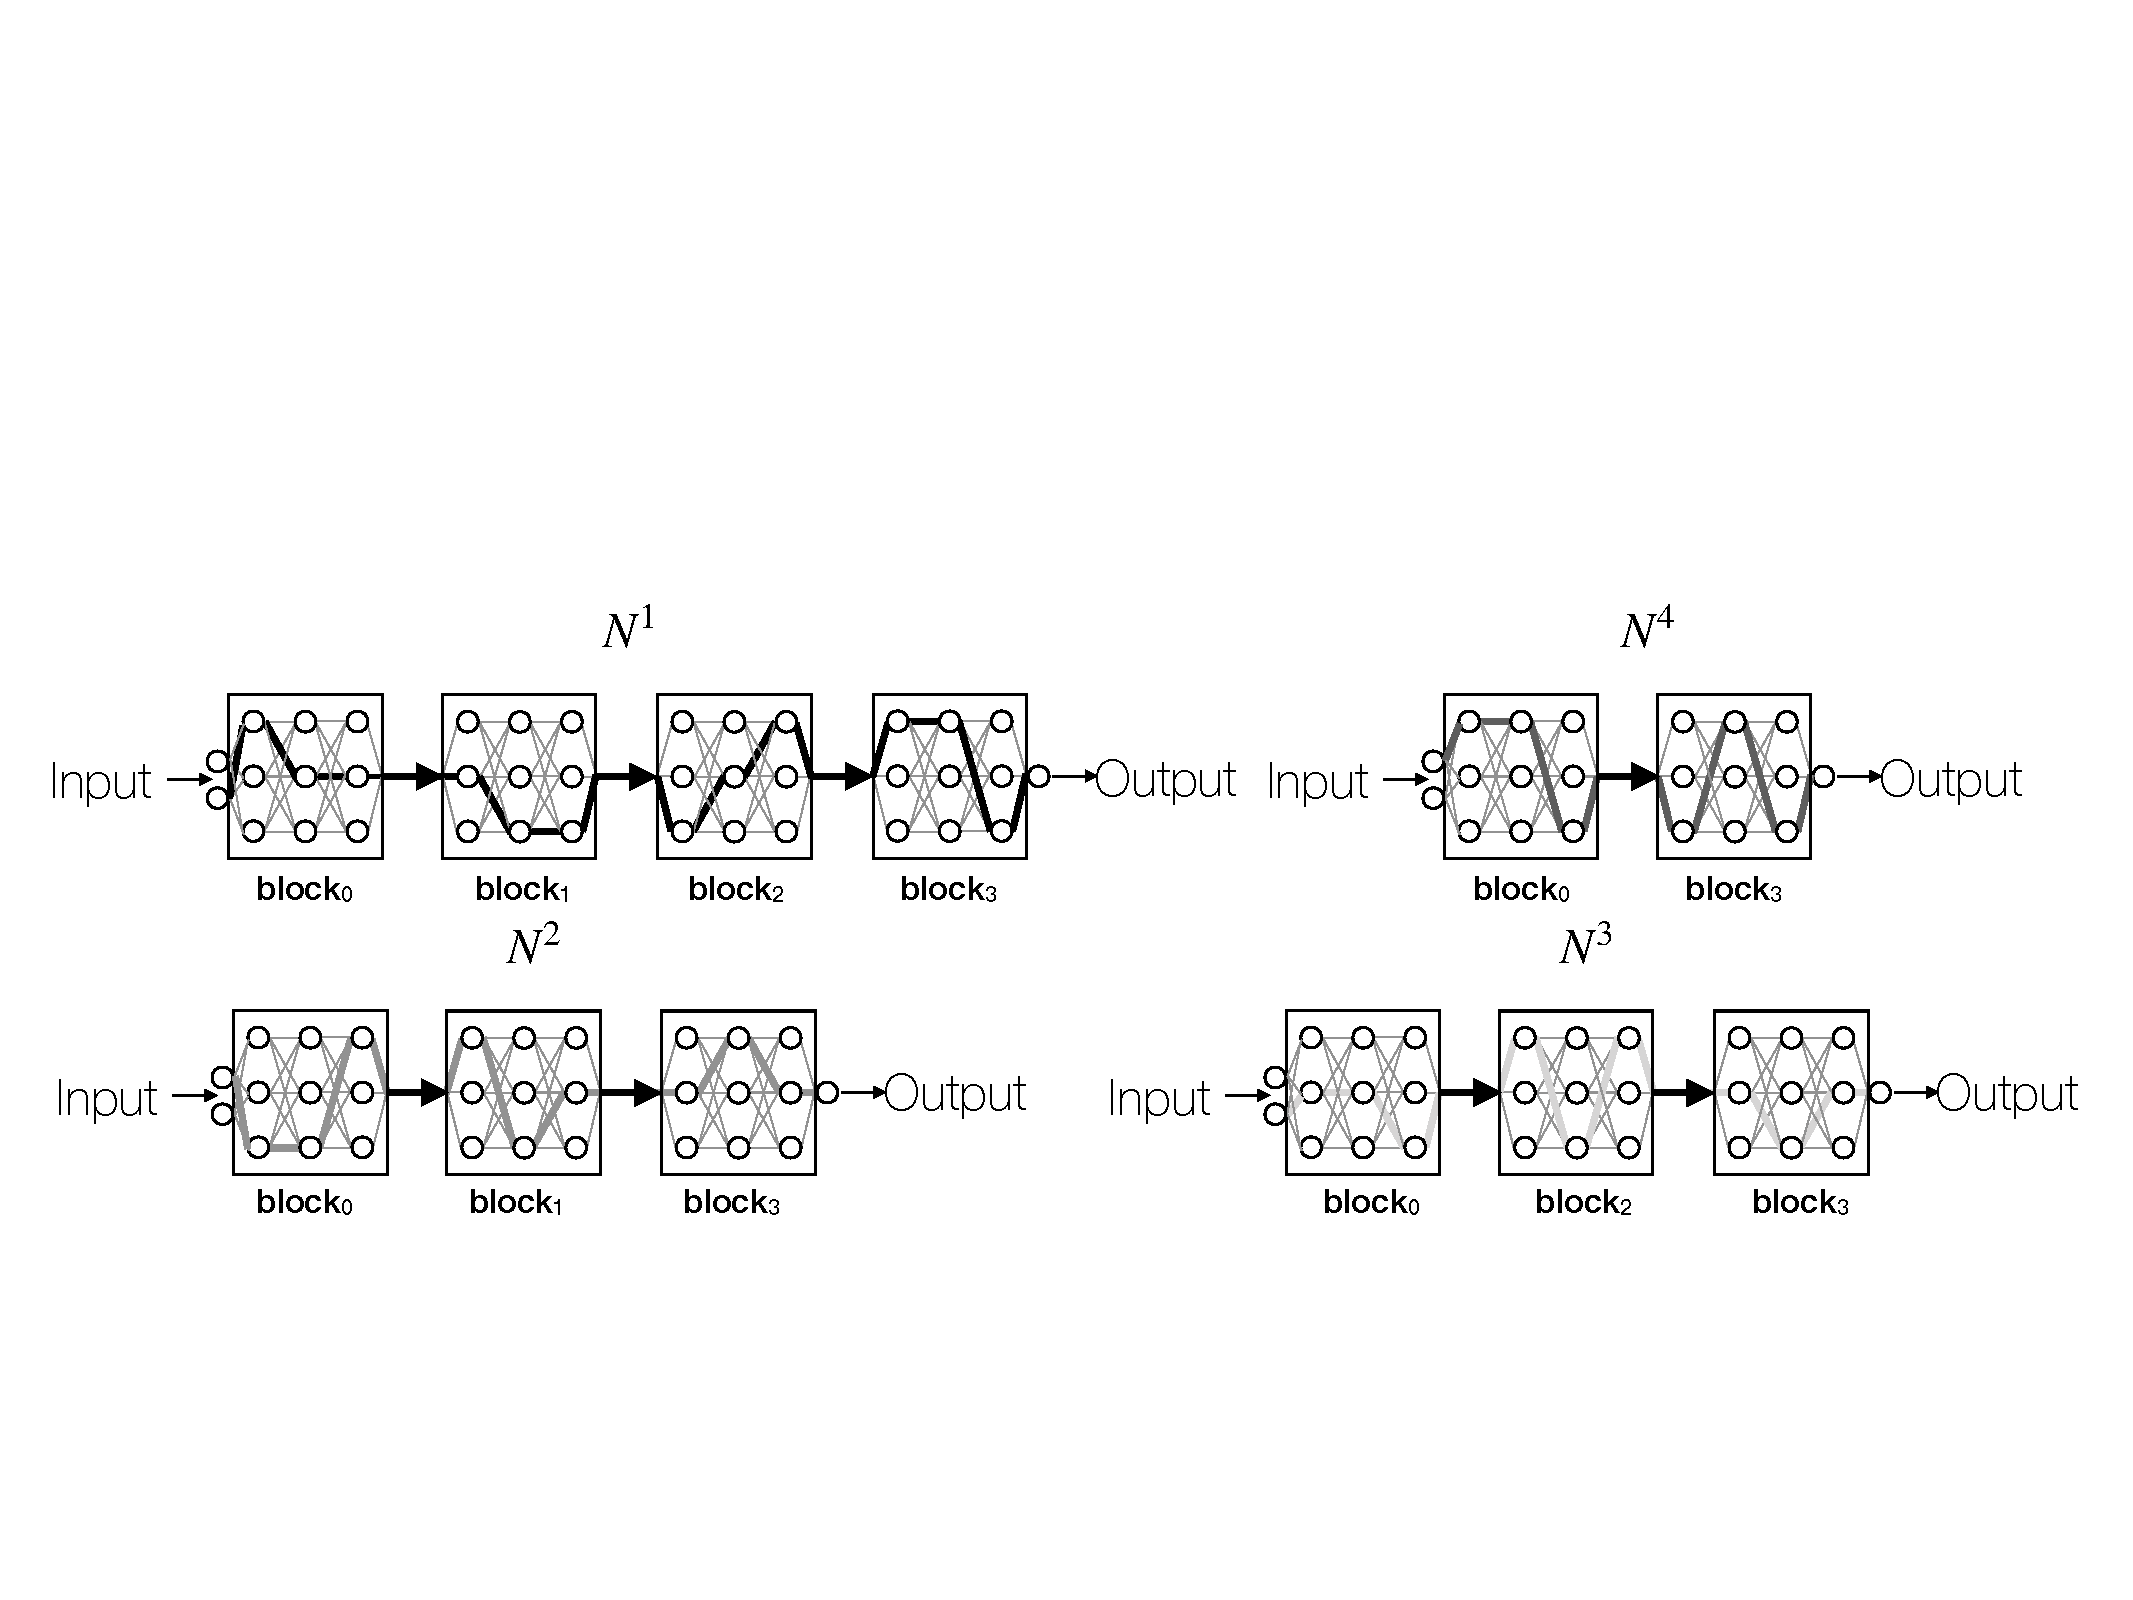
\includegraphics[scale=0.5]{figs/blocks.pdf}
}
\end{minipage}
\caption{\small{On the left is the ResNet with $b$ skip connections and $(b+2)$ blocks. On the right are the sub-FC networks $N^1$ obtained by skipping no blocks, $N^2$ and $N^4$ obtained by skipping block $1$ and $2$ respectively, and $N^3$ obtained by skipping both blocks $1$ and $2$.}}
\label{fig:resnet}
\end{figure}

\begin{definition}\label{def:subfcdnn}[Sub FC-DNNs]
Let $2^{[b]}$ denote the power set of $[b]$ and let $\J\in 2^{[b]}$ denote any subset of $[b]$. Define the`$\J^{th}$' sub-FC-DNN of the ResNet to be the fully connected network obtained by (i) including  $\text{block}_{j},\forall j\in \J$  and (ii) ignoring $\text{block}_{j},\forall j\notin \J$ (see \Cref{fig:resnet}).
\end{definition}
\begin{theorem}[Sum of Product of Kernels Theorem]\label{th:mainres} Let $H^{\J}_{\Tf_0}$ be the NPK of the $\J^{th}$ sub-FC-DNN, and $\bfc^{\J}$ be the associated constant. Under \Cref{assmp:main}, we have:
\begin{align*}
\kv_{\Tdgn_0}\ra \sum_{\J\in 2^{[b]}}  \bfc^{\J} H^{\J}_{\Tf_0}, \,\, \text{as}\,\,  w\ra\infty
\end{align*}
\end{theorem}
\textbf{Note.} The sub-FC-DNNs we refer to in \Cref{th:mainres} belong to (or are parts of) the feature network from which the gates are obtained. 
%\end{comment}
\section{Numerical Experiments}\label{sec:exp} 
In what follows, \Cref{sec:exp1} is themed around the key insight obtained from \Cref{th:main}, i.e., the correlation of the gates lies at the heart of `what is learnt in a DNN with ReLUs'. In particular, we show that operations (such as permuting the layers, tiling cum rotation of the gates, and giving a constant `all-ones' input to the value network) that destroy the layer by layer computational structure do not degrade test performance. These operations lead to combinatorially many models and in all of them the test performance remains the same. In \Cref{sec:exp2} we throw light on the open question in [\citenum{randlabel}] on why test performance degrades due to upstream training with random labels.
% Prior vs now what is the difference : robustness + random label etc
%Datasets are MNIST and CIFAR-10. For MNIST, we use the DGN in \Cref{fig:dgn-prior-new} (right) with fully connected layers instead of the convolutional layers.  All models are trained with `\emph{Adam}'  \cite{adam} (step-size $=3\cdot 10^{-4}$ , batch size $=32$). 
\subsection{Robustness of Gates: Destroying layer-by-layer structure does not affect performance}\label{sec:exp1}
In this experiment we show that information in the gates is invariant even if we destroy the layer-by-layer structure. We consider the three kinds of gates described below.\\
\indent \quad$1.$ \textbf{Fixed Learnt:} We \emph{pre-train} the feature network (which is a DNN with ReLUs), then \emph{freeze} the weights of the feature network, and then train the value network. This way we can measure information in the gates of a trained DNN.\\
\indent \quad$2.$ \textbf{Fixed Random:} We initialise the feature network at random, and then \emph{freeze} its weights and then train the value network. This way we can measure information in the gates of a DNN at initialisation. Here, the feature and value network can be either initialised with the same weights i.e., dependent initialisation (DI) or statistically independent weights  i.e., independent initialisation (II).\\
\indent \quad$3.$ \textbf{Decoupled Learning:} We initialise the weights of the value and feature network statistically independent and then train both of them. For the gradient to flow through the feature network we use \emph{soft-gating}, i.e., $G(q)=\frac{1}{1+\exp({-\beta\cdot q})}$, with $\beta=10$. 

We make use of the deep gated network (DGN) setup shown in \Cref{fig:dgn-prior-new} (right) which is an improvisation of the DGN in prior work [\citenum{npk}] shown in \Cref{fig:dgn-prior-new} (left). In the current setup, {\bf{$G_{i_1},\ldots,G_{i_4}$ is a permutation of the $G_1,\ldots,G_4$}}, which gives $24$ models. Note that these \textbf{permutations destroy the layer by layer structure}. In the prior setup both value and feature networks have the same input $x\in\R^{\din}$. In the current setup, we have two separate inputs, $x^{\text{f}}\in\R^{\din}$ for the feature network and $x^{\text{v}}\in\R^{\din}$ for the value network. We set $x^{\text{f}}=x$ always, however, for $x^{\text{v}}$ there are \textbf{two modes} namely (i) \textbf{standard}: we set $x^{\text{v}}=x$ ,(ii) \textbf{`all-ones'}: we set $x^{\text{v}}=\mathbf{1}\in\R^{\din}$ (a tensor of all $1$'s). While the setup on the left is only one model, the setup on the right has $\mathbf{48=24\times 2}$ \textbf{different models}, where $24=\texttt{factorial}(4)$ is due to the gate permutations and $2$ is due the settings of $x^{\text{v}}$.
\begin{figure}[h]
\centering
\begin{minipage}{0.4\columnwidth}
\centering
\resizebox{\columnwidth}{!}{
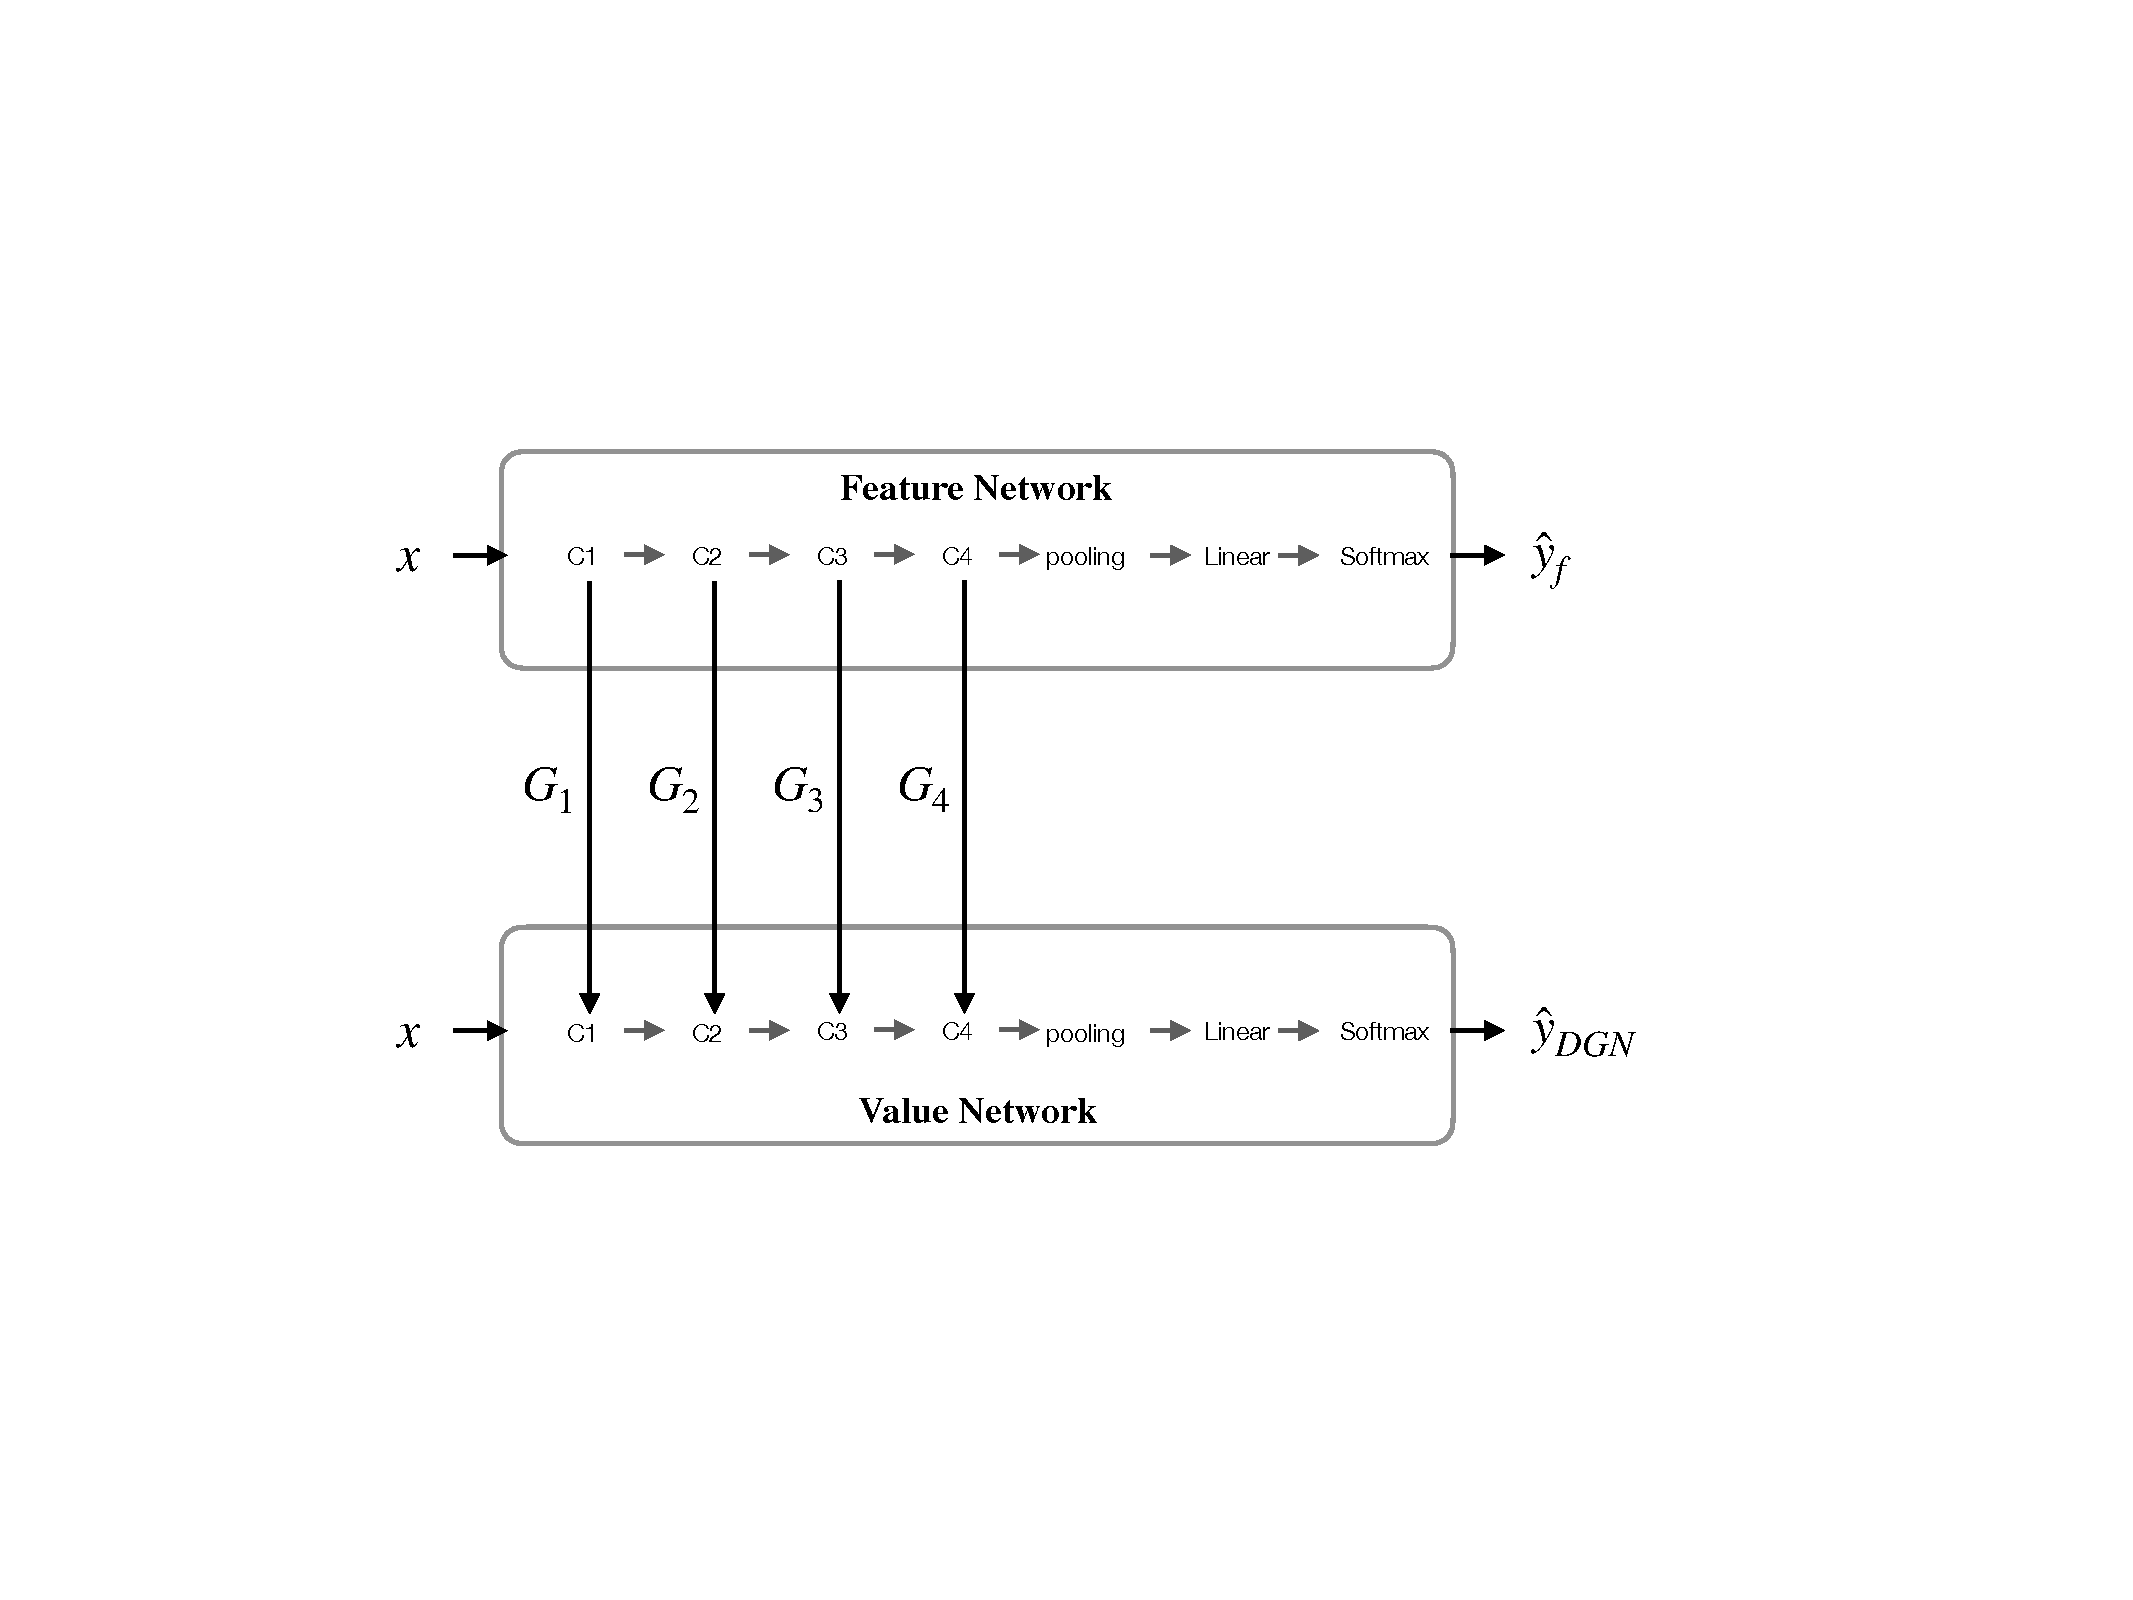
\includegraphics[scale=0.3]{figs/exp-prior.pdf}
}
\end{minipage}
\begin{minipage}{0.4\columnwidth}
\centering
\resizebox{\columnwidth}{!}{
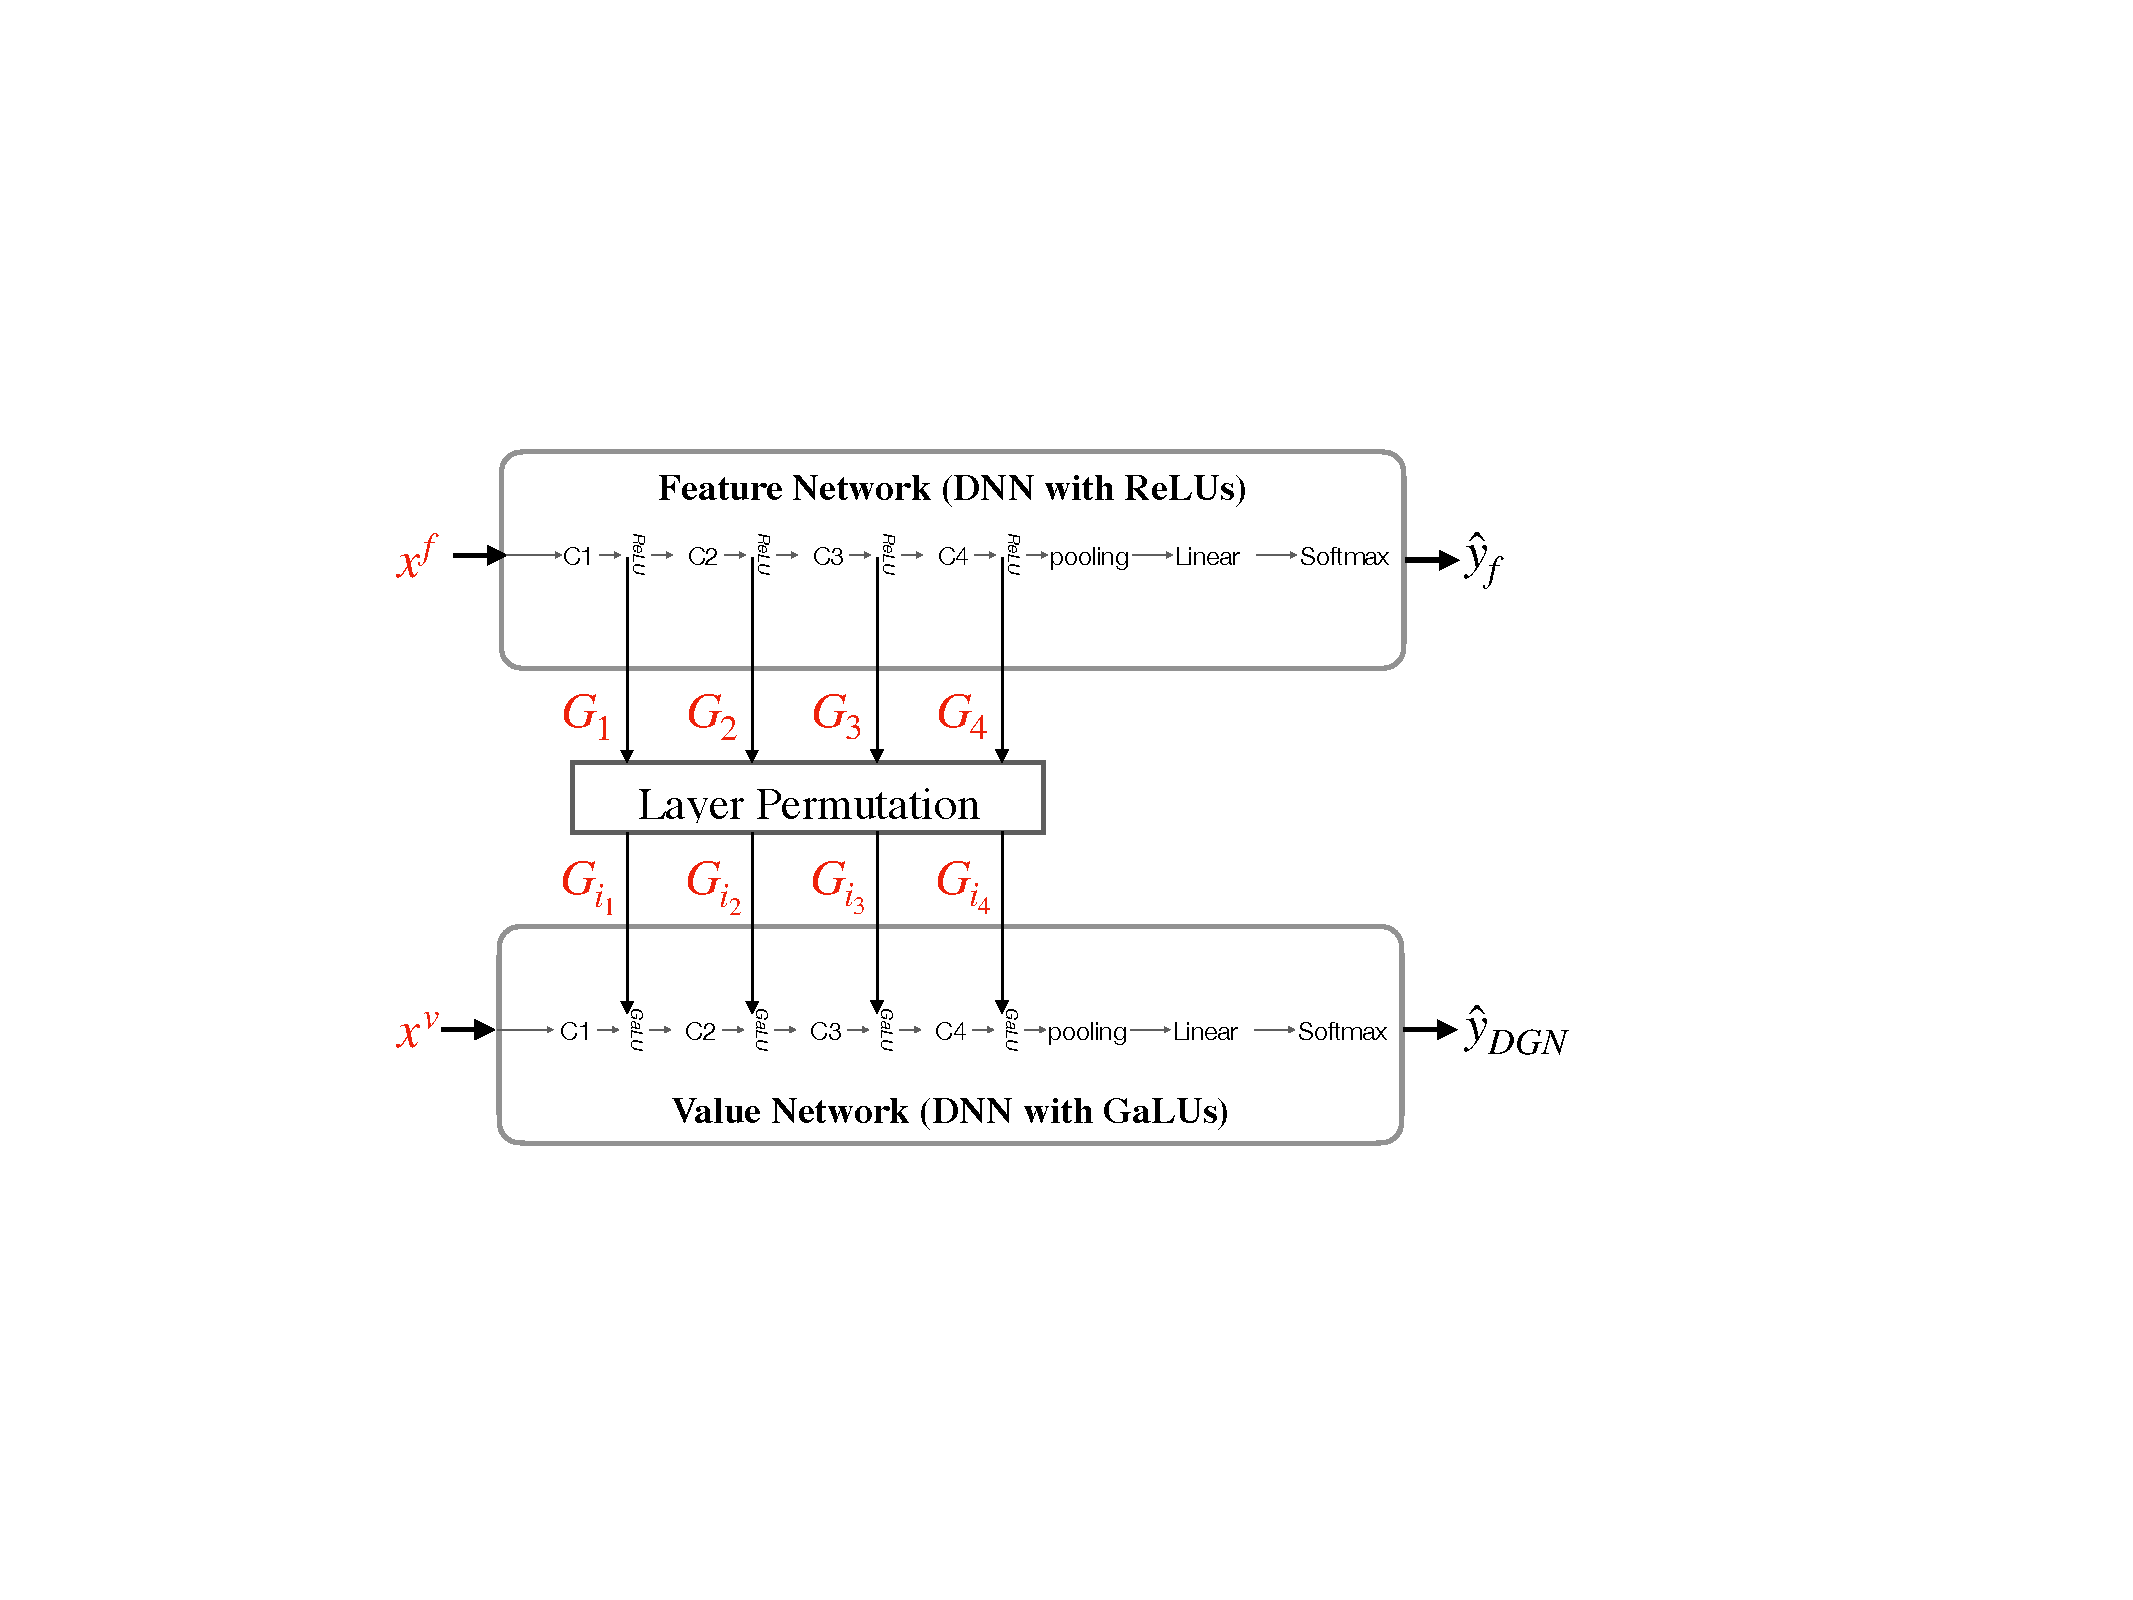
\includegraphics[scale=0.3]{figs/exp-new.pdf}
}
\end{minipage}
\caption{The prior setup in [\citenum{npk}] is shown in the left and the setup in this paper is shown in the right. Here $C1,\ldots,C4$ are convolutional layers with $128$ output filters, kernel size $3\times 3$ and stride $1\times 1$.}
\label{fig:dgn-prior-new}
\end{figure}

\begin{table}[h]
\centering
\begin{minipage}{0.8\columnwidth}
\begin{tabularx}{\columnwidth}{c *{5}{Y}}
\toprule
 Dataset& \multicolumn{2}{c}{Fixed Random}   &  \multicolumn{1}{c}{Decoupled} & \multicolumn{1}{c}{ Fixed } & \multicolumn{1}{c}{ReLU \tiny{(Feature Network)}}\\
& II & DI &Learning &Learnt &\\\hline\arrayrulecolor{white}\midrule
MNIST& 94.1{\tiny{$\pm$0.3}}  &94.1\tiny{$\pm$0.3}  &98.1\tiny{$\pm$0.1} &98.6\tiny{$\pm$0.1} &98.5{\tiny{$\pm$0.1}}\\\hline\\\hline 
CIFAR-10& 67.5\tiny{$\pm$0.7} &67.6\tiny{$\pm$0.7}   &77.6\tiny{$\pm$0.6} &79.4\tiny{$\pm$0.3} &80.4\tiny{$\pm$0.3}\\\hline
\arrayrulecolor{black}\bottomrule
\end{tabularx}
\end{minipage}
\caption{\small Shows the $\%$ test accuracy of various gates. The main result here is that the numbers in columns $1$ to $4$ are averaged over $48$ models (1 run per model, best performance in each run) and performance is robust to layer permutations and $x^{\text{v}}=\mathbf{1}$ input. For ReLU the average is over $5$ independent runs. Optimiser: Adam (3e-4).}
\label{tb:regimes}
\end{table}

\textbf{Note on prior results.} The following two observations were made in prior work [\citenum{npk}]: (i) by using the gates and training the NPV from scratch we can recover the performance (see ReLU vs Fixed Learnt in \Cref{tb:regimes}), and (ii) the performance of  Convolutional NTK ($77.43\%$)[\citenum{arora2019exact}] is between that of finite width network with random gates  ($67.5\%$) and learnt gates give ($79.4\%$), i.e., learning in the gates explains the difference between finite width DNNs and infinite width NTK.

\textbf{Robustness of Gates.} Entries in columns $1$ to $4$ in \Cref{tb:regimes} are  averaged over $48$ different models which included  permuting the layers and providing $\mathbf{1}$ as input. Our main result is that the information in the gates is robust over these $48$ models -- these justify the insights from \Cref{th:main} that as long as correlation in the gates is not destroyed the performance does not degrade. We also went one step further with respect to destroying the structure by considering arbitrary rotations. Here, we first tile the gates of the various filters (as a tensor) in the reverse order starting from layer $4$ to layer $1$ and then rotate arbitrarily in each of the three dimension for five times as shown in left of \Cref{fig:visual-permute} (i.e, two image dimensions and one filter dimension). For each rotation in the filter dimension we choose a random integer belonging to  $[0,512)$ and for each of the rotation in the image dimensions we choose a uniform random integer belonging to $[0,32)$. We did $10$ independent runs of the fixed learnt gates and decoupled learning of gates and observed the test performance to be $79.4${\tiny$\pm$0.2} and $79.0${\tiny$\pm$0.5} respectively (which are similar to the numbers shown in \Cref{tb:regimes}).

\begin{figure}[h]
\begin{minipage}{0.3\columnwidth}
\resizebox{\columnwidth}{!}{
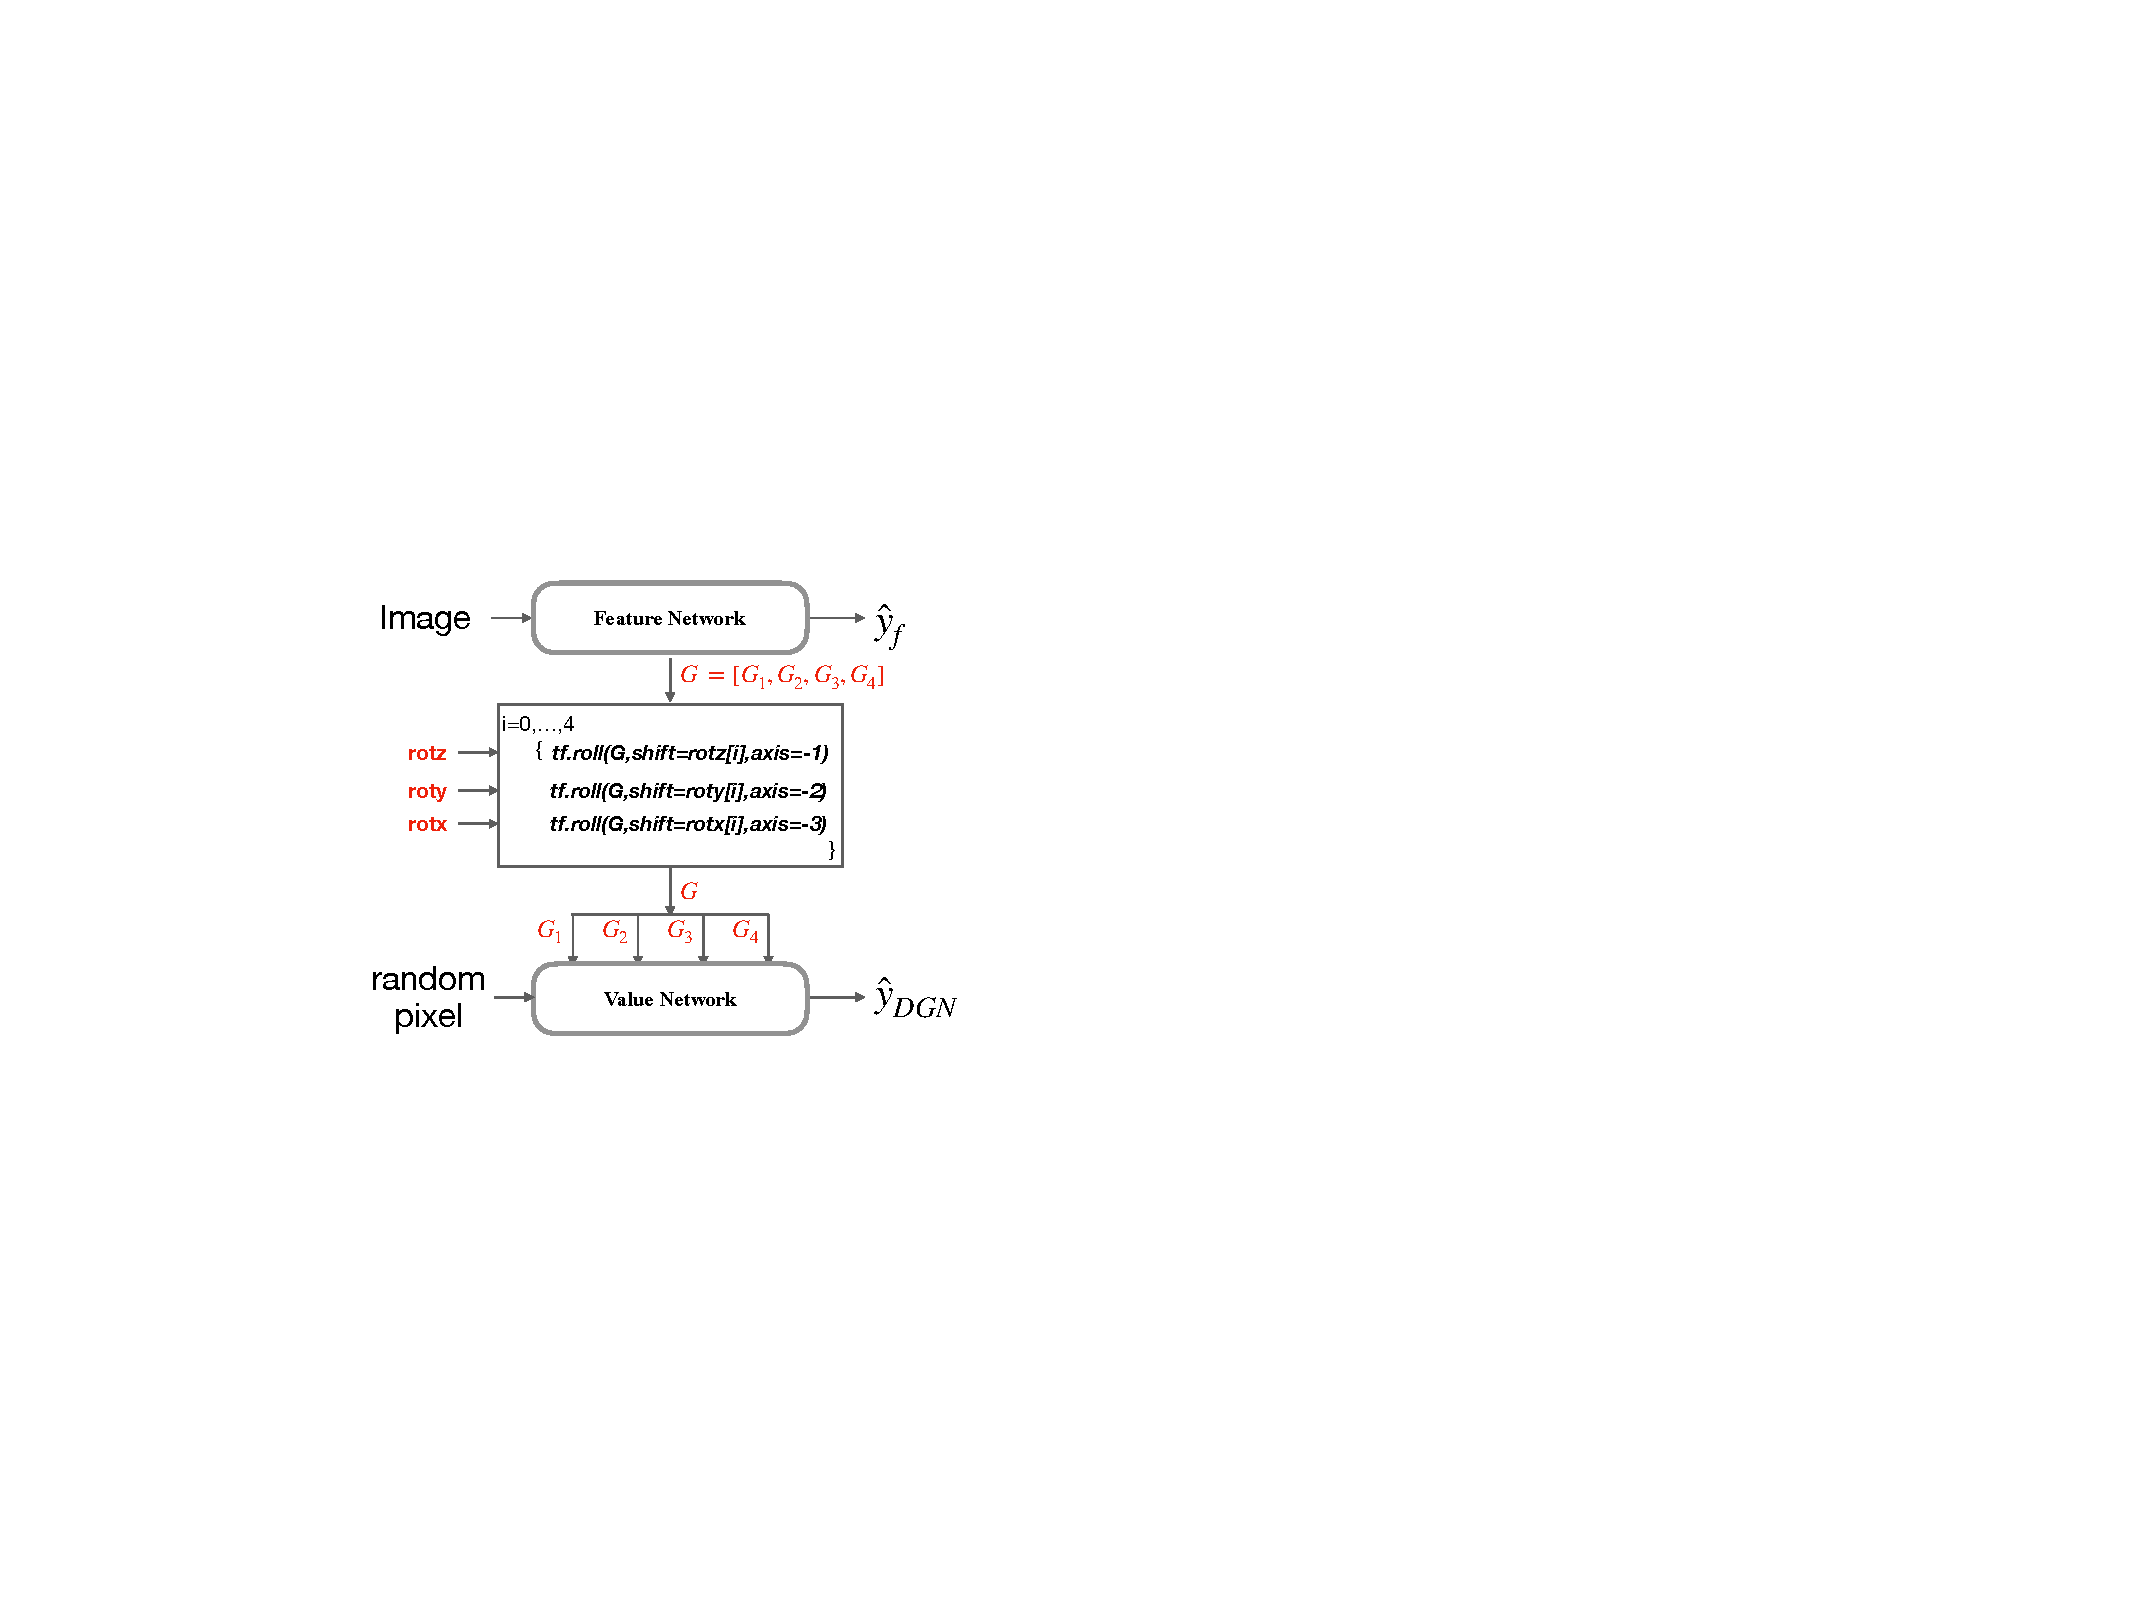
\includegraphics[scale=0.25]{figs/arbitrary_shift.pdf}
}
\end{minipage}
\begin{minipage}{0.68\columnwidth}
\resizebox{\columnwidth}{!}{
\begin{tabular}{cccccccccc}
&\Huge{Input}& \Huge{Layer 1, Filter 1}& \Huge{Layer 1, Filter 2}& \Huge{Layer 2, Filter 1}& \Huge{Layer 2, Filter 2}& \Huge{Layer 3, Filter 1}& \Huge{Layer 3, Filter 2}& \Huge{Layer 4, Filter 1}& \Huge{Layer 4, Filter 2}\\
\Huge{Feature Network}&\includegraphics{visual-iclr/images/horse.png}&
\includegraphics{images_neurips_2021/feature_network/layer_1_0.png}&
\includegraphics{images_neurips_2021/feature_network/layer_1_1.png}&
\includegraphics{images_neurips_2021/feature_network/layer_2_0.png}&
\includegraphics{images_neurips_2021/feature_network/layer_2_1.png}&
\includegraphics{images_neurips_2021/feature_network/layer_3_0.png}&
\includegraphics{images_neurips_2021/feature_network/layer_3_1.png}&
\includegraphics{images_neurips_2021/feature_network/layer_4_0.png}&
\includegraphics{images_neurips_2021/feature_network/layer_4_1.png}\\
\Huge{Value Network}&\includegraphics{images_neurips_2021/allones.png}&
\includegraphics{images_neurips_2021/value_network//layer_1_0.png}&
\includegraphics{images_neurips_2021/value_network//layer_1_1.png}&
\includegraphics{images_neurips_2021/value_network//layer_2_0.png}&
\includegraphics{images_neurips_2021/value_network//layer_2_1.png}&
\includegraphics{images_neurips_2021/value_network//layer_3_0.png}&
\includegraphics{images_neurips_2021/value_network//layer_3_1.png}&
\includegraphics{images_neurips_2021/value_network//layer_4_0.png}&
\includegraphics{images_neurips_2021/value_network//layer_4_1.png}
\end{tabular}
}

\end{minipage}
\caption{Top (Standard CNN): First image on the left is the input image and the next $8$ images are outputs of $2$ filters in each of the $4$ layers. Bottom (DGN with gates of the top model applied in reverse order): First image on the left is the input to the value network and the next $8$ images are outputs of $2$ filters in each of the $4$ layers. Both models achieve a test accuracy of about $80\%$.}
\label{fig:visual-permute}
\end{figure}

\textbf{Primal vs Dual View of features.} The standard (primal) view is that the input is processed layer-by-layer and the hidden features are in the layer outputs. 
%The dual view is that the features are encoded in the gates (analytically speaking the NPF/NPK). While both are mathematically equivalent, we believe that the dual view paints more accurate picture. 
Our experiments challenge the primal view, because, 
we do not provide the image as input but only $\mathbf{1}$ (`all-ones') as input to the value network, and we have destroyed the layer-by-layer structure of the gates before applying them as masks in the value network as well.  As a result, there is a huge `visual' difference between the hidden layer outputs of the feature network and that of the value network (see right of \Cref{fig:visual-permute}).  One could still insist that DNNs are so powerful that they are recovering the features layer-by-layer. Or alternatively, one can appeal to the dual view to conclude that since neither `all-ones' input nor the arbitrary rotation of the gates affect the correlation of gates (\Cref{th:main}), the performance does not degrade. While the gates are generated layer-by-layer in the feature network, when applied as masks, the function of the gates is to learn and train the paths and sub-networks (viewpoint trivially following from \Cref{prop:npf-npv}) .


\begin{comment}
\textbf{Primal vs Dual View of features.} The standard (primal) view is that the input is processed layer-by-layer and the hidden features are in the layer outputs. To challenge this view, 
%The dual view is that the features are encoded in the gates (analytically speaking the NPF/NPK). While both are mathematically equivalent, we believe that the dual view paints more accurate picture. Our experiments challenge the primal view. 
we do not provide the image as input but only $\mathbf{1}$ (`all-ones') as input to the value network. Now, it could be argued that the value network gets the information about the via its gating masks. To counter this argument, we have destroyed the layer-by-layer structure of the gates before applying them as masks in the value network as well. As a result, there is a huge `visual' difference between the hidden layer outputs of the feature network and that of the value network (see right of \Cref{fig:visual-permute}).  One could still insist that DNNs are so powerful that they are recovering the features layer-by-layer. Or alternatively, one can appeal to the dual view to conclude that since neither `all-ones' input nor the arbitrary rotation of the gates affect the correlation of gates (\Cref{th:main}), the performance does not degrade. While the gates are generated layer-by-layer in the feature network, when applied as masks, the function of the gates is to learn and train the paths and sub-networks (viewpoint trivially following from \Cref{prop:npf-npv}) .
\end{comment}

\textbf{Gate learning need not be layer-by-layer.} Note that  in `decoupled learning' of gates (column $3$ \Cref{tb:regimes}), while the gates are generated layer-by-layer in the feature network, after permutations/arbitrary rotations they end in a completely different location in the value network during training. Thus even during training, the gates can be arbitrarily placed.

\subsection{Upstream training with random labels and downstream with true labels affects the gates}\label{sec:exp2}


\textbf{Q1 (open question [\citenum{randlabel}]).} {When trained with random labels upstream followed by true labels downstream, the test performance of a DNN with ReLUs degrades, Why?}

\textbf{Setup to answer Q1.} We hypothesise that the answer to the above question lies in the gates. To test our hypothesis, we train in two phases (i) Phase I: upstream training with label noise levels $\gamma=0, 25\%, 50\%, 75\%$ and (ii) Phase II: downstream training with true labels. For $\gamma=0$ there is no Phase II because Phase I is already with true labels. We then measure the information stored in the gates at the end of each of the two phases. To this end, we consider the DGN setup in \Cref{fig:dgn-prior-new} (left), and train the feature network (which is a DNN with ReLUs). In Phase I, we train the feature network for different values of label noise $\gamma=0, 25\%, 50\%, 75\%$, which gives us models $M1(\gamma)$ (see \Cref{fig:rand-label-setup}). To measure the information in the gates learnt at the end of Phase I, we keep these gates fixed and train the value network with true labels -- this gives us models $M2(\gamma)$ (see \Cref{fig:rand-label-setup}). In Phase II, we start with models $M1(\gamma)$, and perform downstream training with true labels to obtain models $M4(\gamma)$.  To measure the information in the gates learnt at the end of Phase II, we keep these gates fixed and train the value network with true labels -- this gives us models $M5(\gamma)$ (see \Cref{fig:rand-label-setup}).

\begin{figure}[h]
\centering
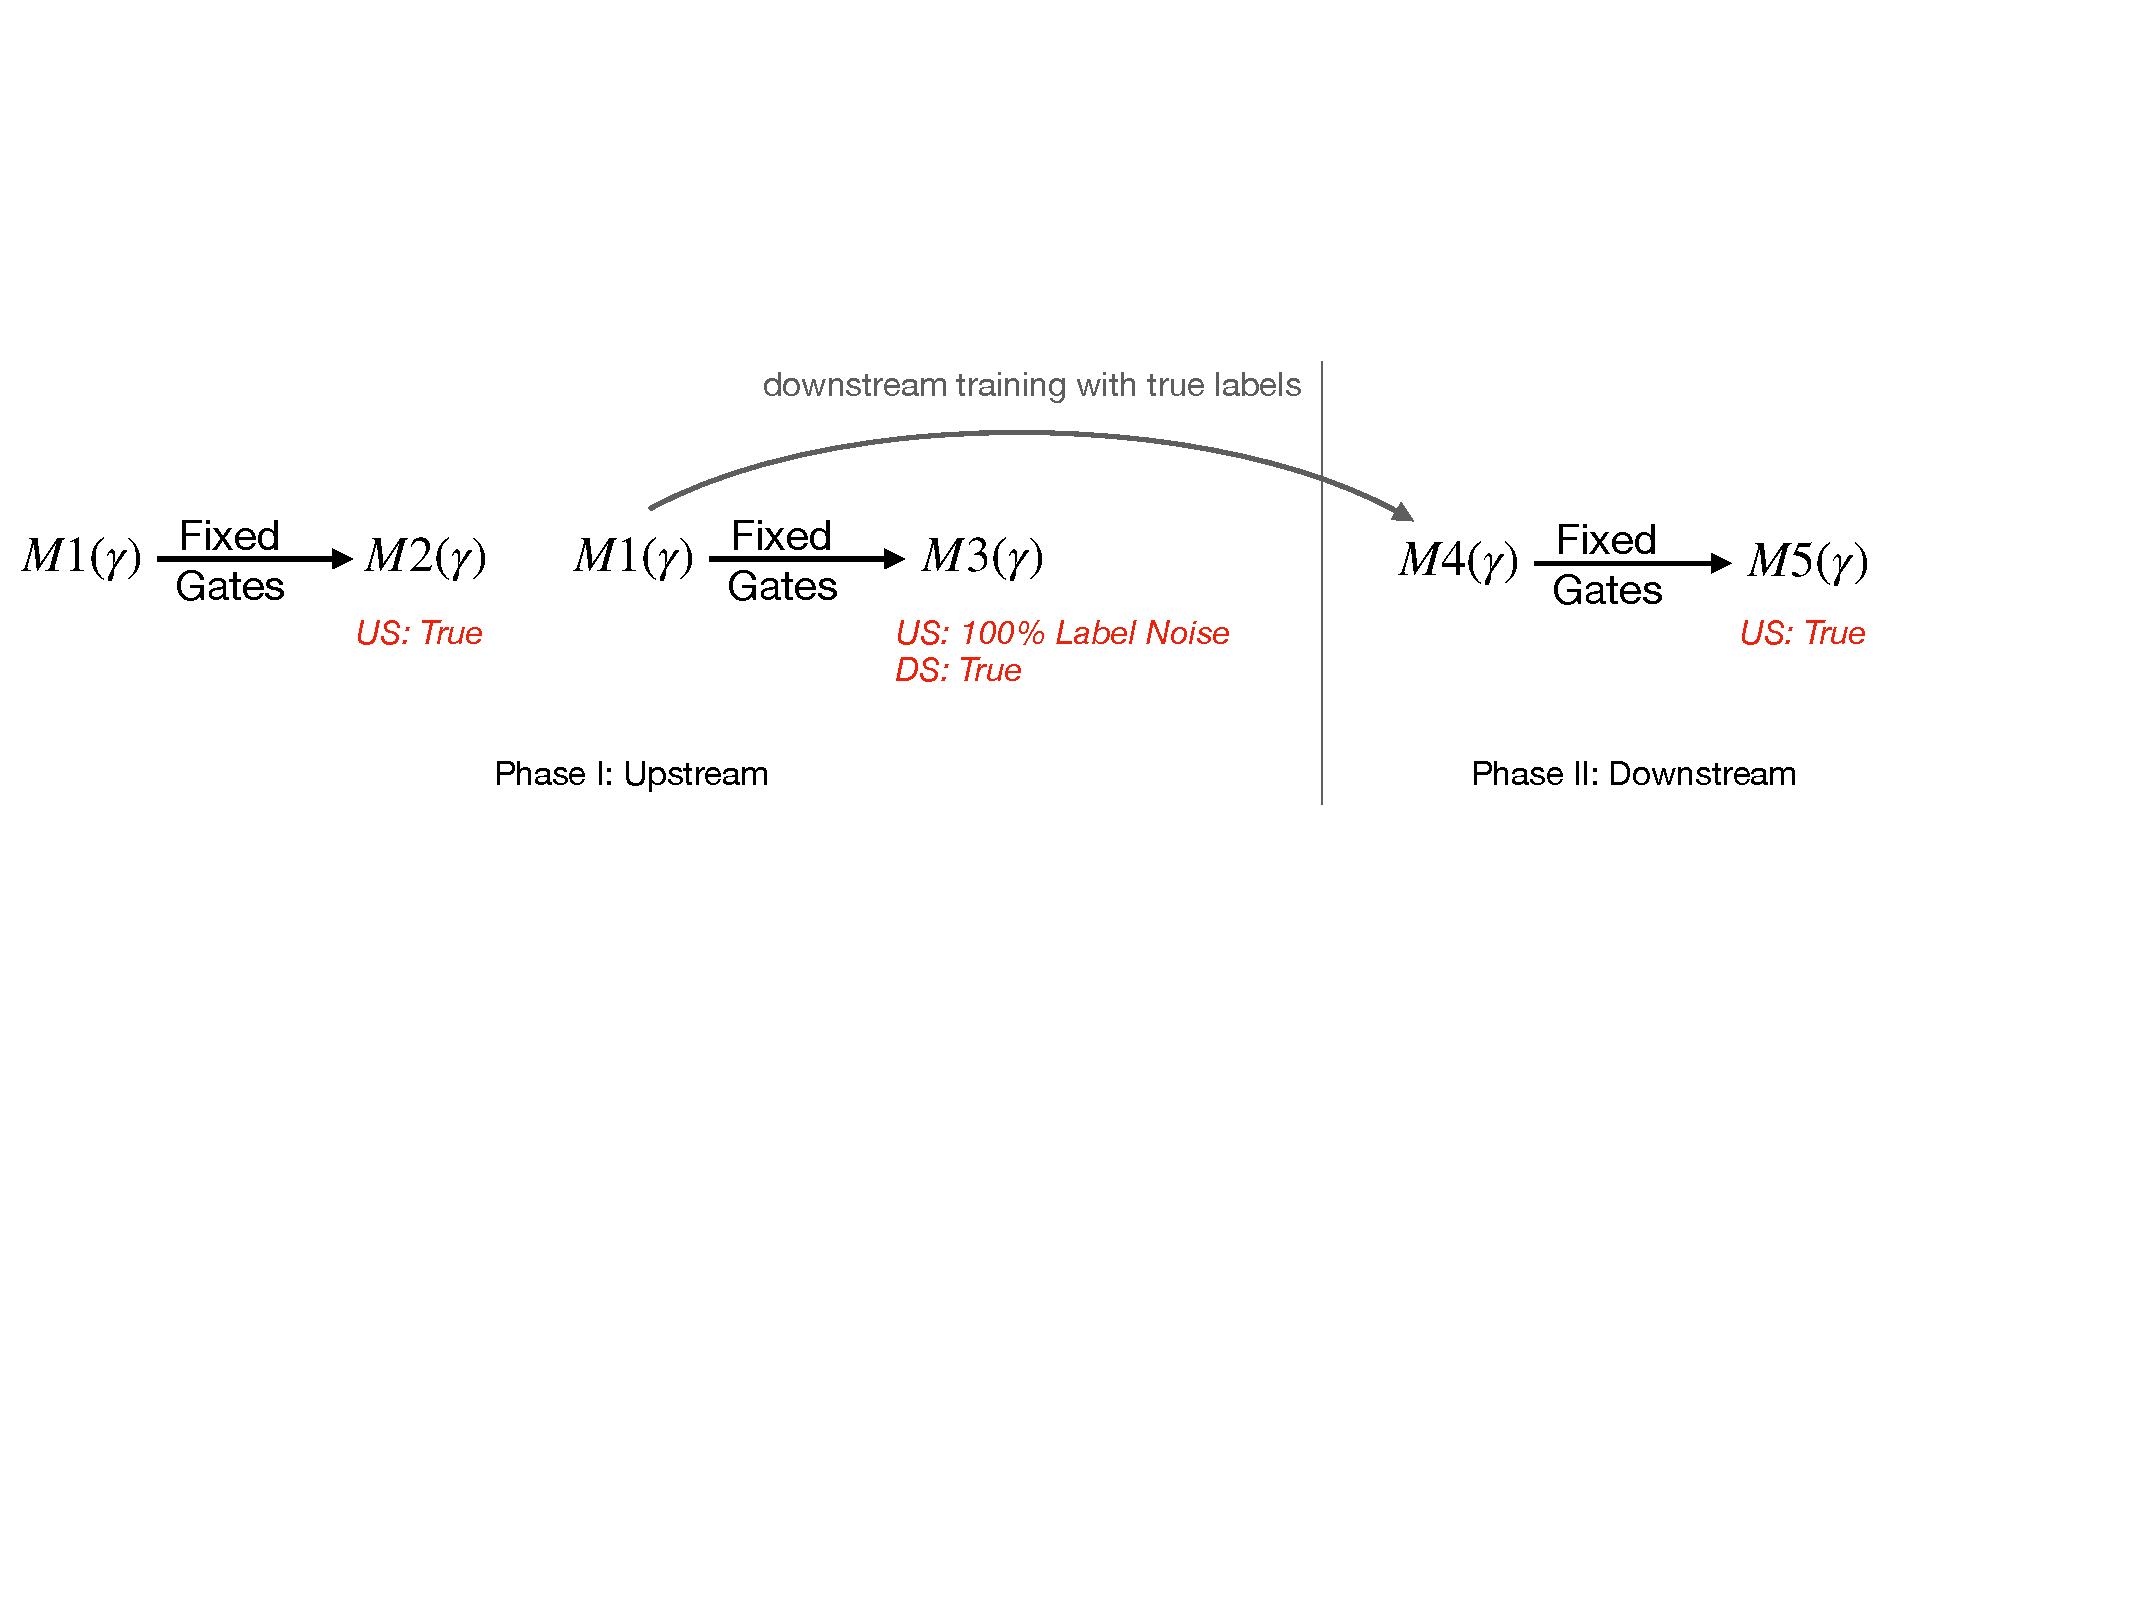
\includegraphics[scale=0.3]{figs/rand-label-big.pdf}
\caption{Shows various models trained in Experiment 2. Here, US and DS stand for upstream and down stream respectively. True for training with true labels. Here models $M1$ and $M4$ are feature networks (DNNs with ReLUs), and $M2, M3$ and $M5$ are value networks which use the fixed gates from the feature networks. Models are parameterised by $(\gamma)$ which is the label noise level.}
\label{fig:rand-label-setup}
\end{figure}


\textbf{Q2 (new question).} {When trained with random labels upstream followed by true labels downstream, \emph{if the gates are fixed throughout and only the weights are trained}, does the test performance degrade?}

\textbf{Setup to answer Q2.} Here, we pick up the models trained at the end of Phase I, use them as feature networks and fix the gates. We then train the value network, first upstream with with $100\%$ random labels, and then downstream with $100\%$ true labels--this gives us models $M3(\gamma)$.

We now discuss the results of the experiments with random labels shown in \Cref{tb:rand-label}.

\textbf{Answer to Q2.} \emph{When the gates are fixed test performance is robust to upstream training with random labels.} In  \Cref{tb:rand-label}, look at the performance of $M3(\gamma=0)$ and compare it performance of  $M4(\gamma), \gamma=25,50,75$. When the gates are fixed, the upstream training with even $100\%$ label noise does not hurt the test performance so much ($81.2-79.3 <2\%$) in comparison to the cases when the gates are allowed to change (as it is the case of DNN with ReLUs), the test performance degrades (from $81.2$) to $76.9$ ( $ 4.3\%$ for $\gamma=25$), $73.6$ ( $7.6\%$ for $\gamma=50$) and  $68.1$ ($13.1\%$ for $\gamma=75$) for even less than $100\%$ label noise.



\begin{table}[h]
\begin{tabularx}{\columnwidth}{c *{6}{Y}}
\toprule
 & \multicolumn{4}{c}{Phase I: Upstream}  
 & \multicolumn{2}{c}{Phase II: Downstream}\\
\cmidrule(lr){2-5} \cmidrule(l){6-7}
&  \multicolumn{2}{c}{ReLU}  &\multicolumn{2}{c}{Fixed Gates} & ReLU & {Fixed Gates}\\
\cmidrule(lr){2-3} \cmidrule(lr){4-5}\cmidrule(lr){6-7}
$\gamma$& Best & End & True& US/DS & True & True\\\hline\arrayrulecolor{white}\midrule
0 &{\bf{81.2}}{\tiny $\pm$ 0.3} & 80.0{\tiny $\pm$ 0.4} &{\bf{80.3}}{\tiny $\pm$ 0.2} & {\bf{79.3}}{\tiny $\pm$ 0.4} &-&- \\\hline\hline
{25}&76.1{\tiny $\pm$ 0.6} & 63.1{\tiny $\pm$ 0.7}& 74.7{\tiny $\pm$ 0.5}& 72.3{\tiny $\pm$ 0.2}&76.9{\tiny $\pm$ 0.1}&76.9{\tiny $\pm$ 0.4}\\\hline\hline
{50}&70.9{\tiny $\pm$ 0.8} & 41.5{\tiny $\pm$ 1.1}& 69.9{\tiny $\pm$ 0.3} & 66.8{\tiny $\pm$ 0.1}&73.4{\tiny $\pm$ 0.3}&73.6{\tiny $\pm$ 0.4}\\\hline\hline
{75}&56.9{\tiny $\pm$ 0.4} & 23.4{\tiny $\pm$ 0.4}& 63.9{\tiny $\pm$ 0.4} &60.0{\tiny $\pm$ 0.3}&68.1{\tiny $\pm$ 0.4}&67.7{\tiny $\pm$ 0.6}\\\hline
\arrayrulecolor{black}\bottomrule
Models & \multicolumn{2}{c}{M1($\gamma$)} & M2($\gamma$) & M3($\gamma$)& M4($\gamma$) & M5($\gamma$)\\\bottomrule
\end{tabularx}
\caption{\small Shows the test accuracy on CIFAR-10 of the various models in Experiment 2. The numbers are averaged over $3$ runs (best accuracy is taken in each run except for column `End'). Optimiser: Adam(3e-4).}
\label{tb:rand-label}
\end{table}


\textbf{Answer to Q1.} \emph{When training with random labels upstream, the test performance degrades because the gates get degraded.} This follows from the fact that the performance of the DNN with ReLUs at the end of Phase II, i.e., $M4$ and that of the value network with the fixed gates at end of Phase II, i.e., $M5$ are approximately equal (within $0.5\%$). 

\textbf{Gates are fairly robust to random labels.} Note that while training with random labels upstream, the test performance initially improves, reaches a peak and then degrades (see columns `Best' and `End' in \Cref{tb:rand-label}). The performance of the DNN with ReLUs at the end of `Phase I' is shown in the column `End' of \Cref{tb:rand-label}. However, the performance of the fixed gates at the end of `Phase I' shown in third column of \Cref{tb:rand-label} is much better and is more closer to the performance of the downstream model $M4$. This means, during upstream training with random labels, the performance degradation post the peak value mostly affects only the weights and not the gates.

\begin{comment}
\begin{figure}[h]
\begin{minipage}{0.99\columnwidth}
\resizebox{\columnwidth}{!}{
\begin{tabular}{ccc}
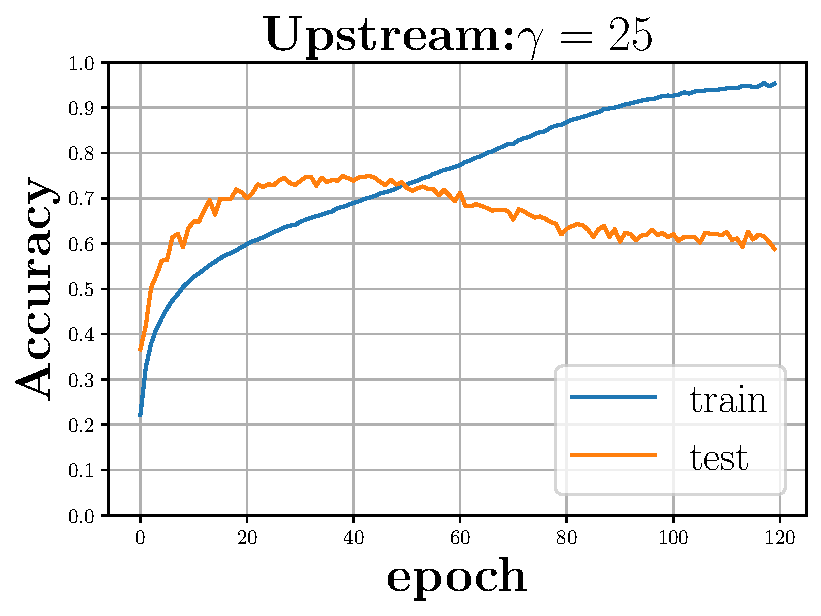
\includegraphics[scale=0.125]{figs/relu_25.pdf}&
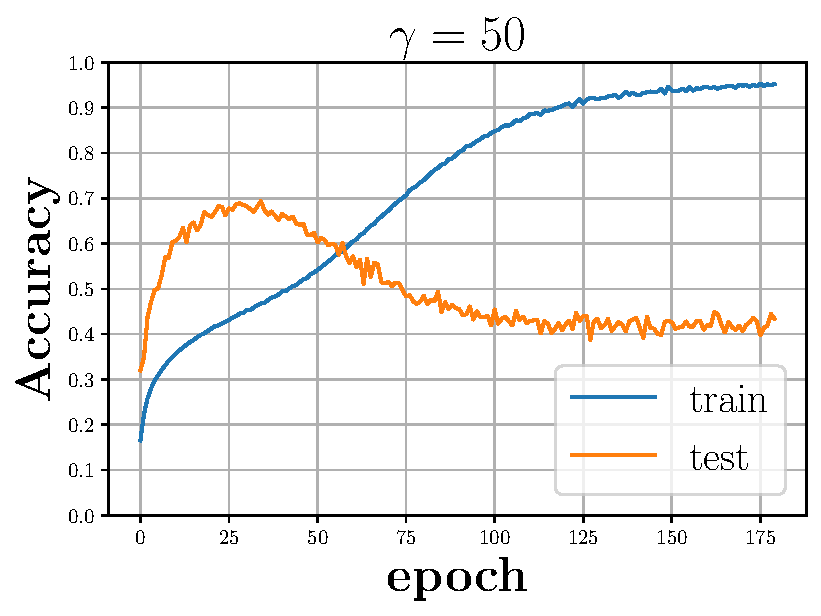
\includegraphics[scale=0.125]{figs/relu_50.pdf}&
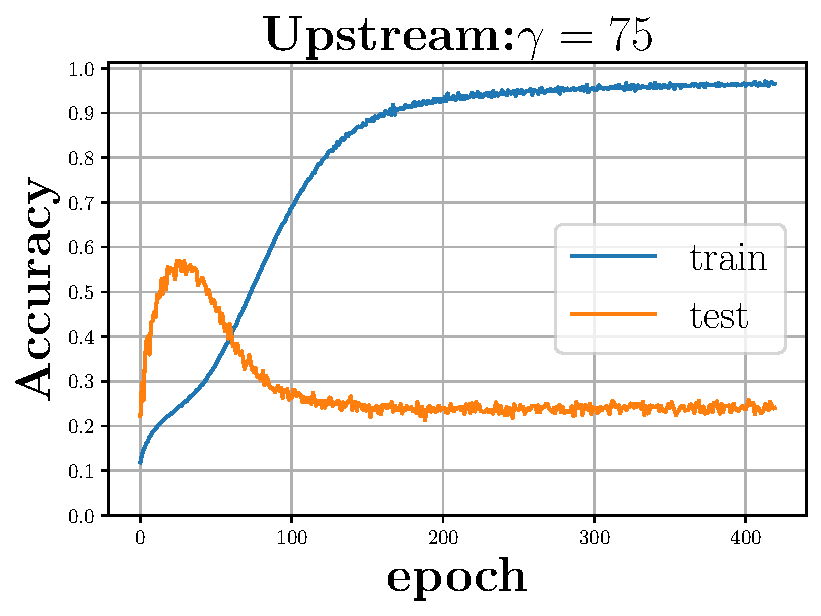
\includegraphics[scale=0.125]{figs/relu_75.pdf}
\\
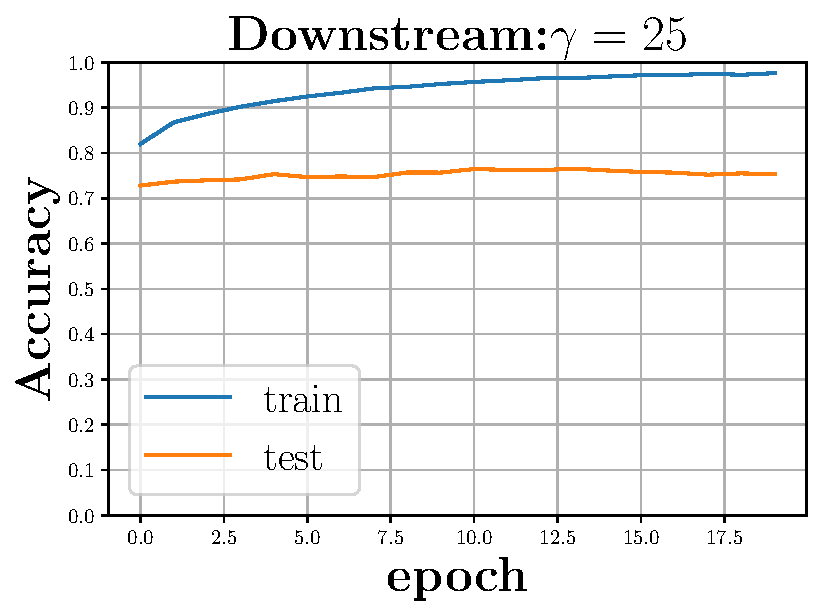
\includegraphics[scale=0.125]{figs/relu_25_good.pdf}&
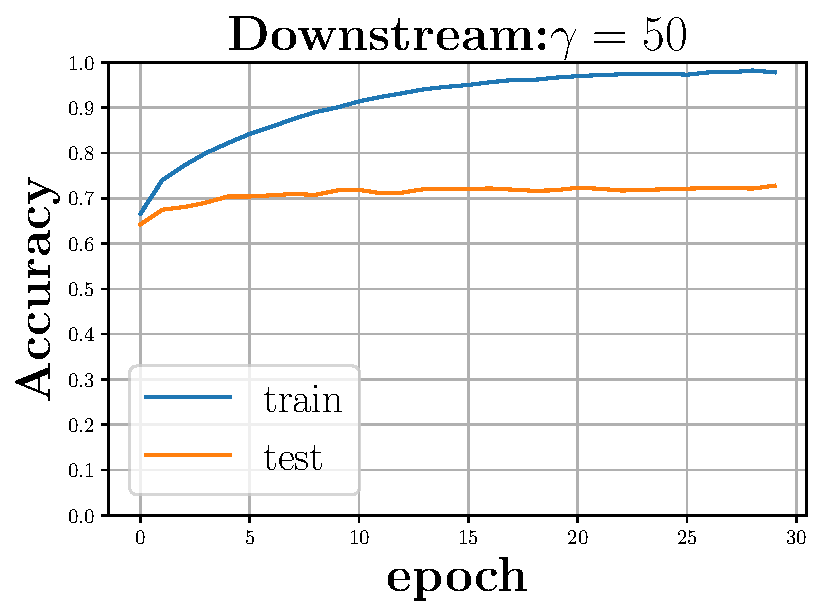
\includegraphics[scale=0.125]{figs/relu_50_good.pdf}&
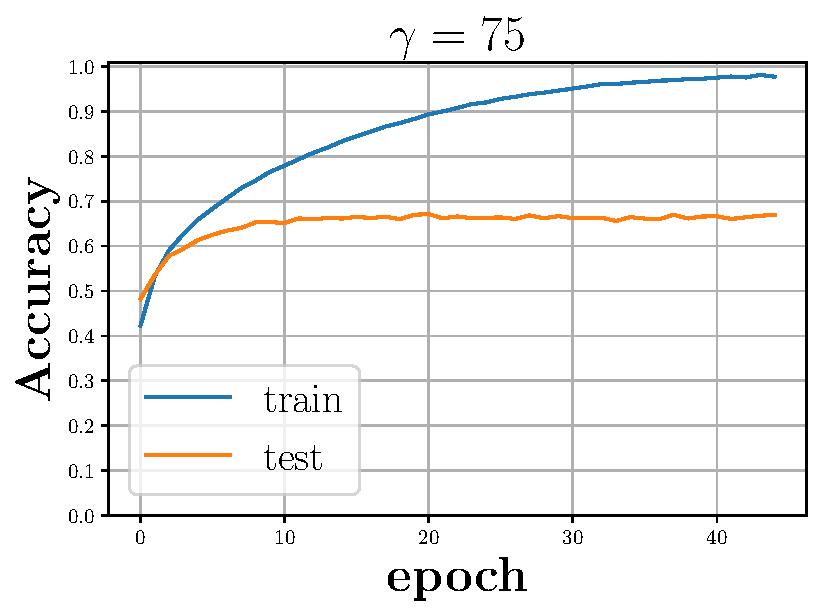
\includegraphics[scale=0.125]{figs/relu_75_good.pdf}\\
\end{tabular}
}
\end{minipage}
\caption{Shows the upstream training with random labels followed downstream training with true labels. The first epochs of bottom plots is same as the epoch follows the last epoch in the top plots.}
\label{fig:rand-label}

\end{figure}
\end{comment}

\begin{comment}
\begin{figure}[h]
%\begin{comment}
\begin{minipage}{0.4\columnwidth}
\resizebox{\columnwidth}{!}{
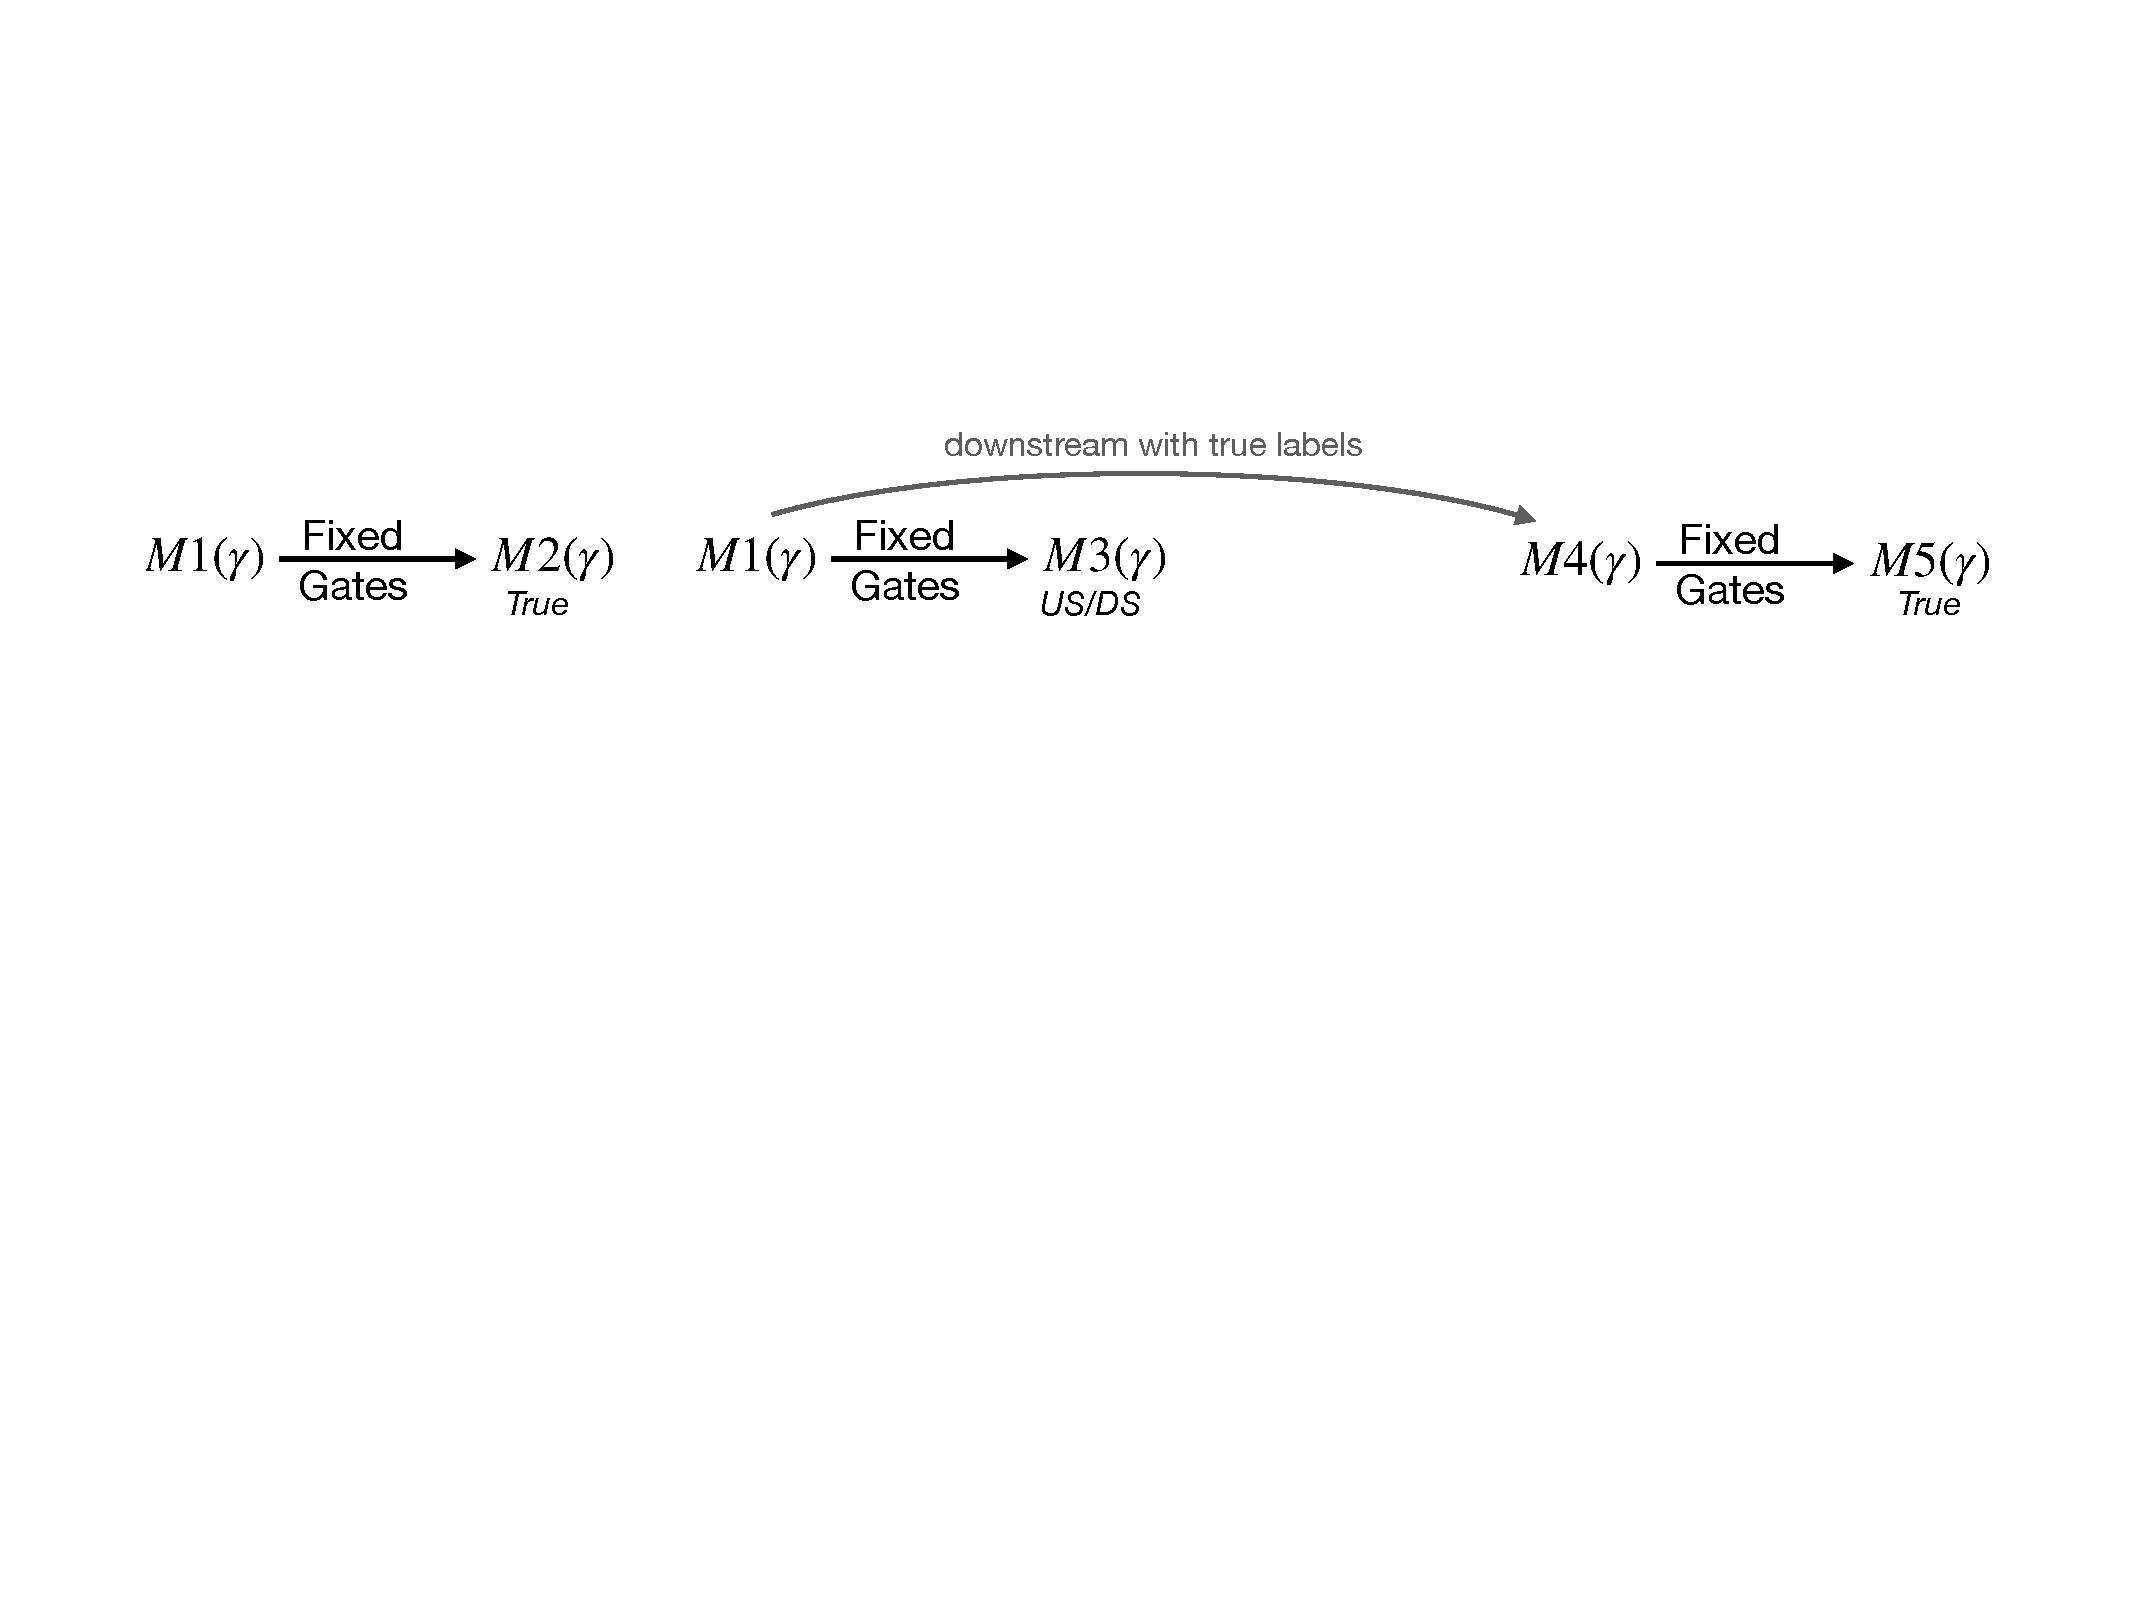
\includegraphics[scale=0.35]{figs/rand-label.pdf}
}
\end{minipage}
%\end{comment}
\begin{minipage}{0.99\columnwidth}
\resizebox{\columnwidth}{!}{
\begin{tabular}{cccccc}
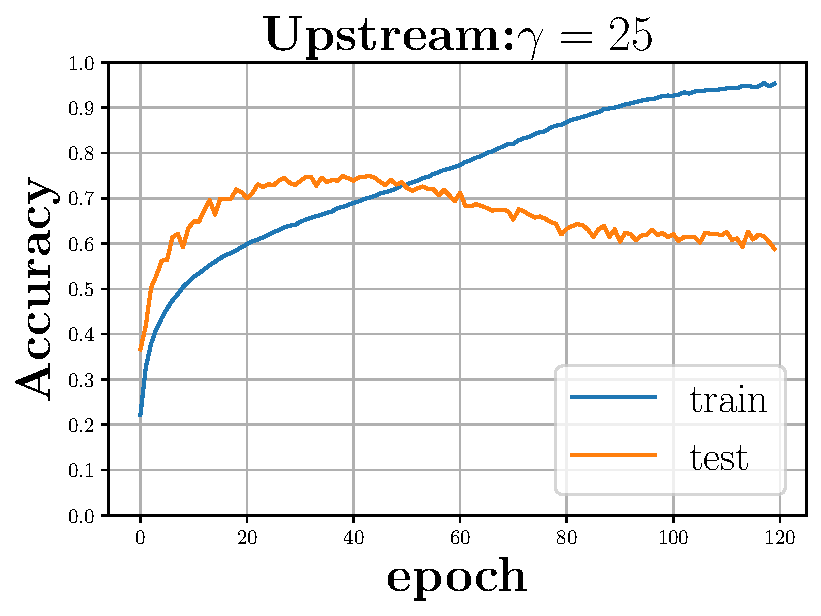
\includegraphics[scale=0.125]{figs/relu_25.pdf}&
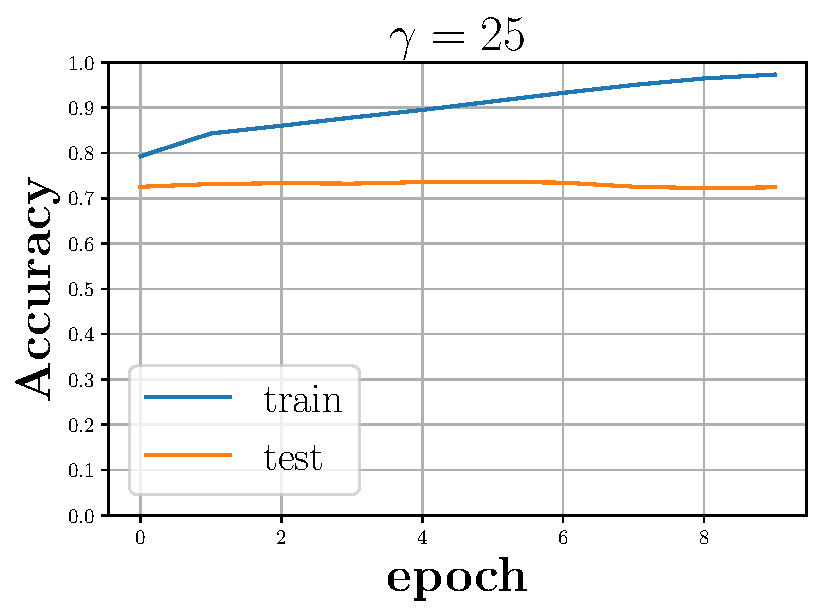
\includegraphics[scale=0.125]{figs/galu_25_good.pdf}&
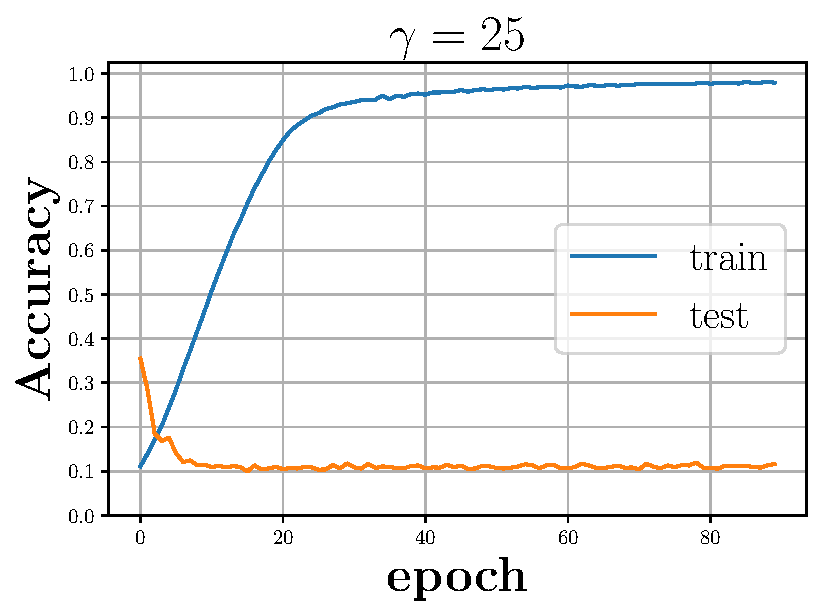
\includegraphics[scale=0.125]{figs/galu_25_bad.pdf}&
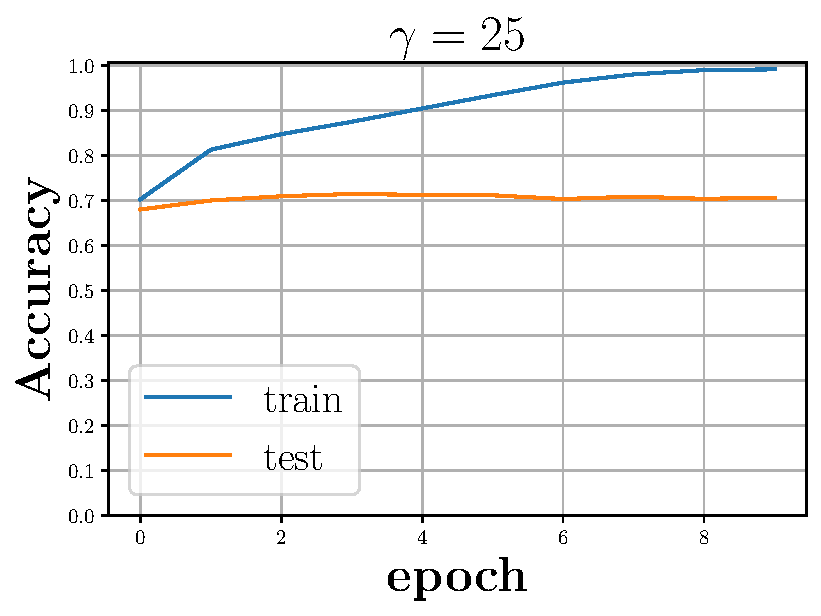
\includegraphics[scale=0.125]{figs/galu_25_bad_good.pdf}&
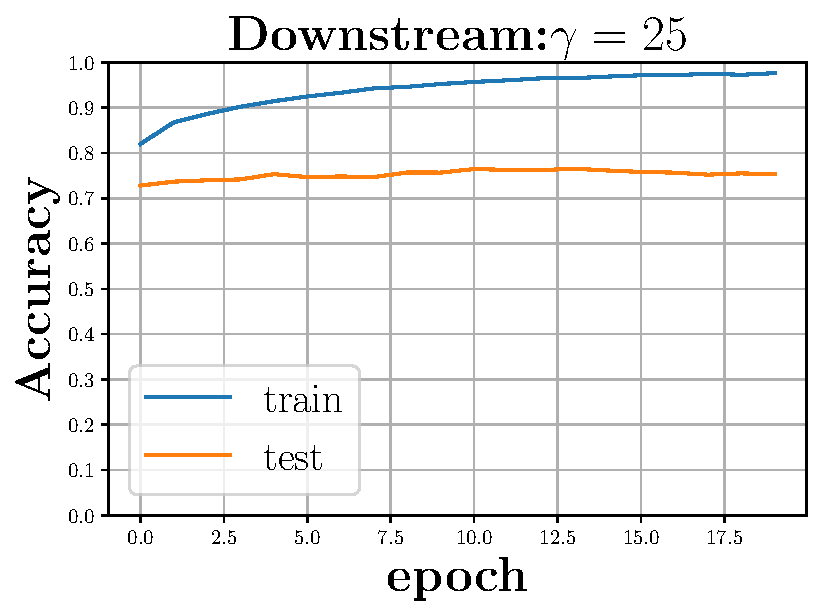
\includegraphics[scale=0.125]{figs/relu_25_good.pdf}&
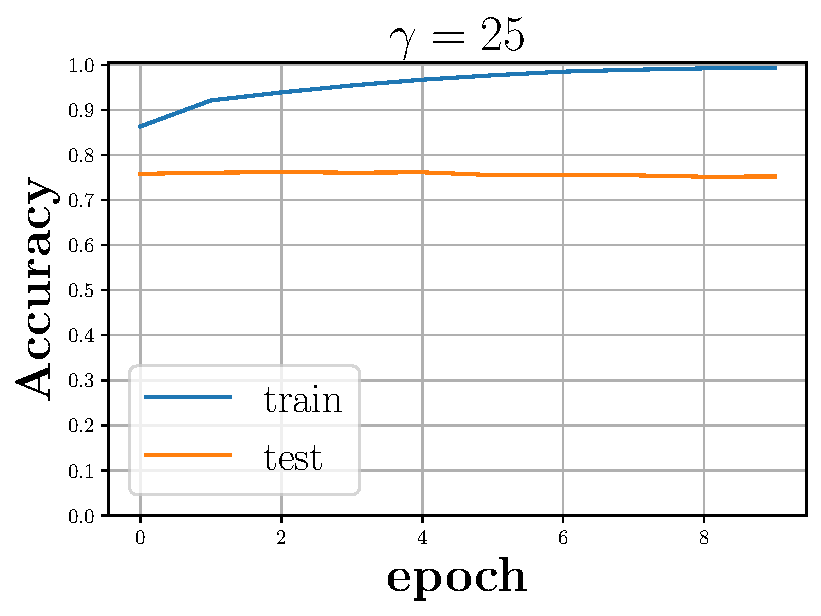
\includegraphics[scale=0.125]{figs/galu_25_recovered.pdf}
\\
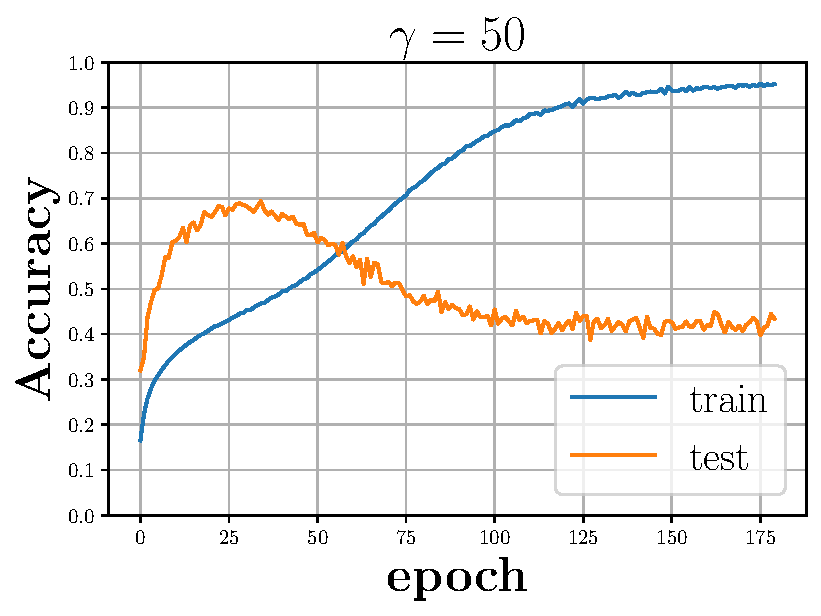
\includegraphics[scale=0.125]{figs/relu_50.pdf}&
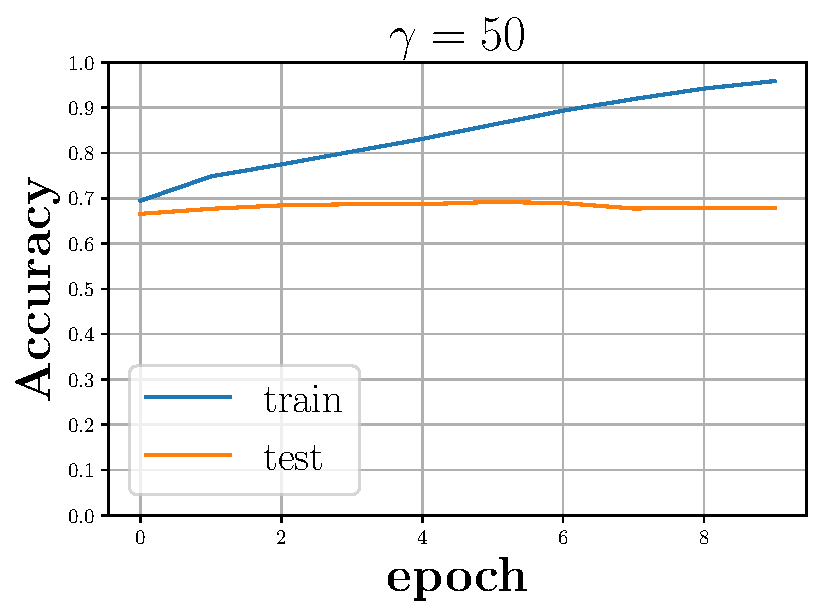
\includegraphics[scale=0.125]{figs/galu_50_good.pdf}&
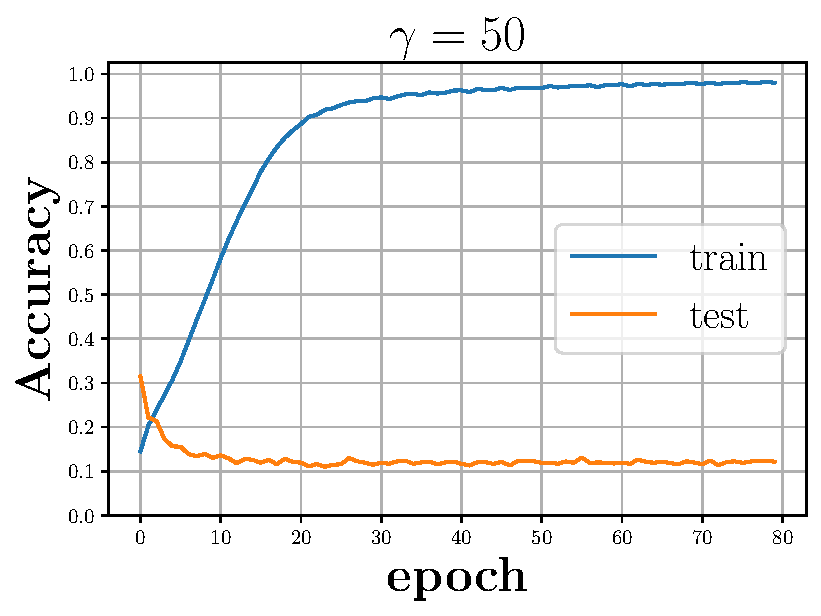
\includegraphics[scale=0.125]{figs/galu_50_bad.pdf}&
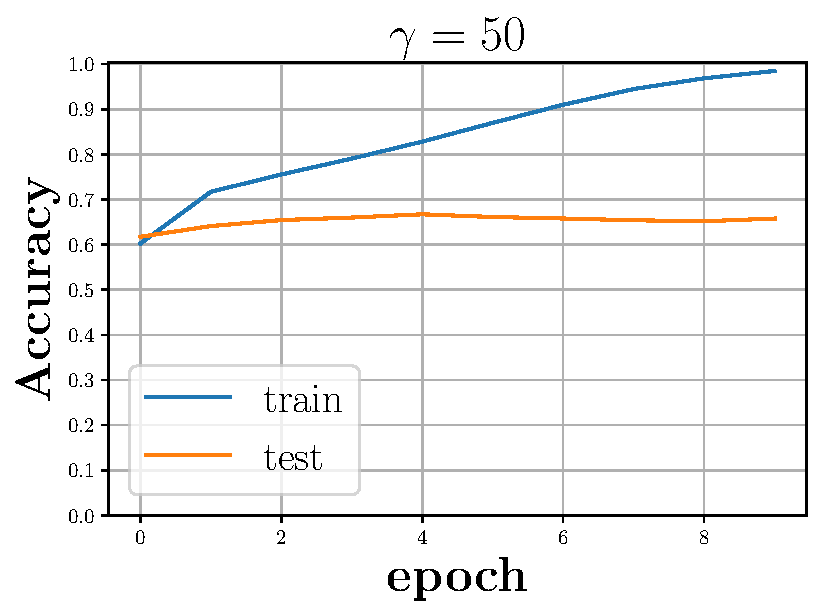
\includegraphics[scale=0.125]{figs/galu_50_bad_good.pdf}&
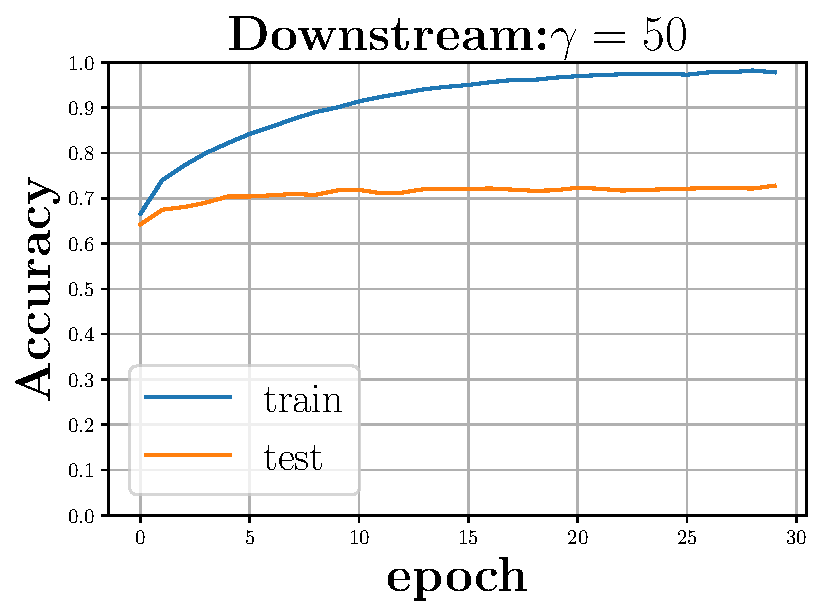
\includegraphics[scale=0.125]{figs/relu_50_good.pdf}&
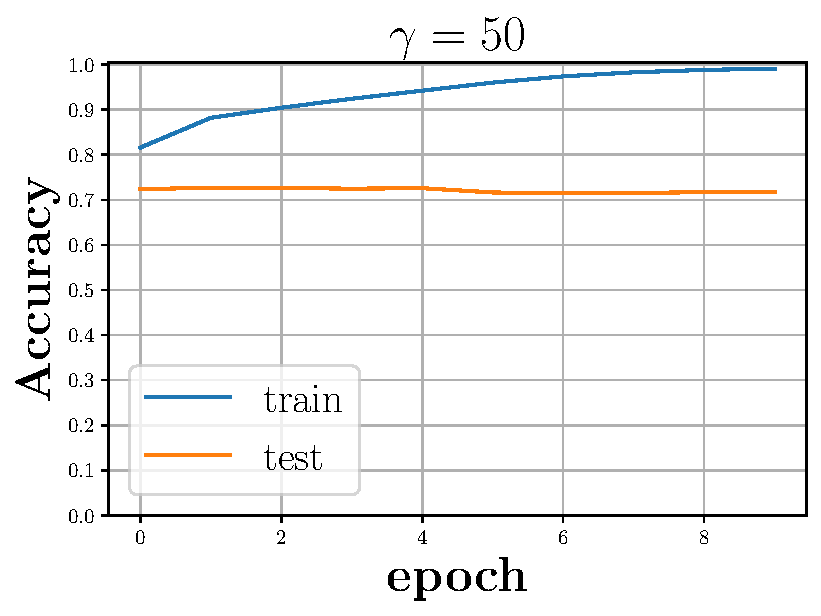
\includegraphics[scale=0.125]{figs/galu_50_recovered.pdf}
\\
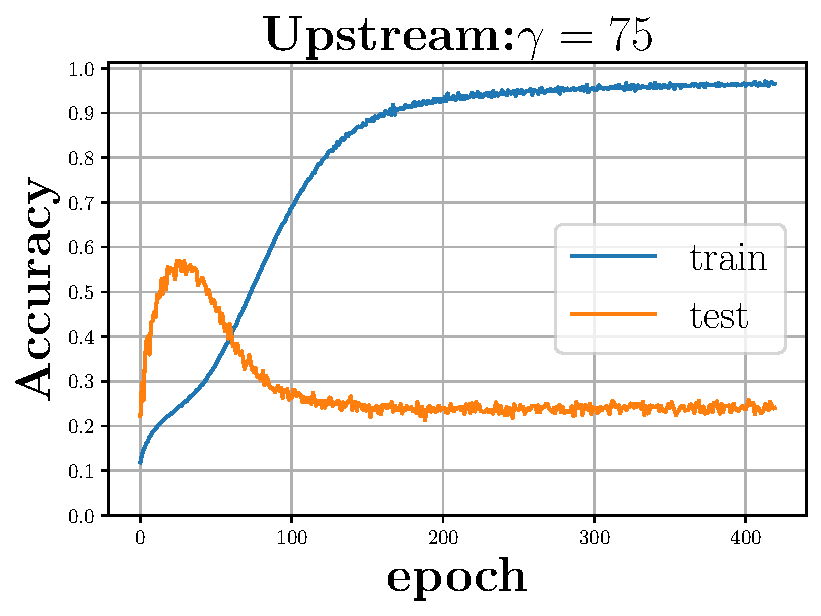
\includegraphics[scale=0.125]{figs/relu_75.pdf}&
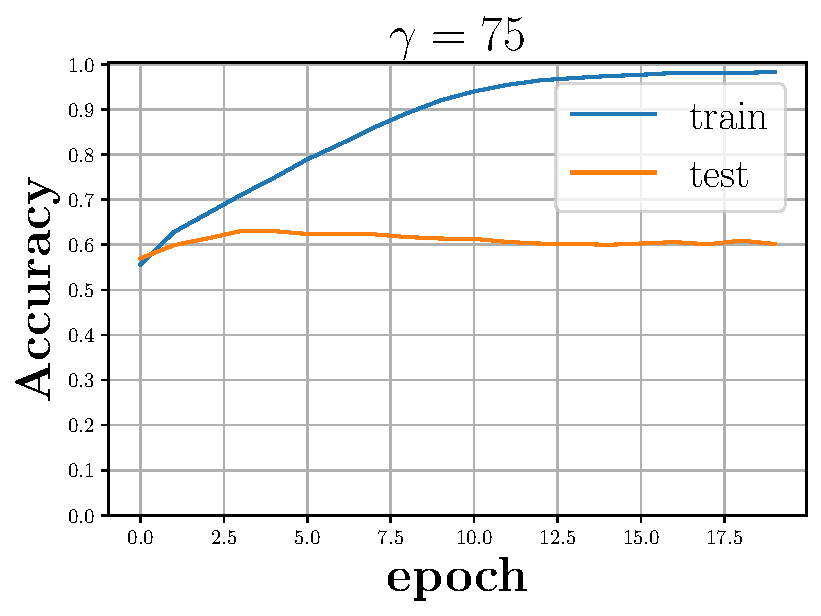
\includegraphics[scale=0.125]{figs/galu_75_good.pdf}&
\includegraphics[scale=0.125]{figs/galu_75_bad.pdf}&
\includegraphics[scale=0.125]{figs/galu_75_bad_good.pdf}&
\includegraphics[scale=0.125]{figs/relu_75_good.pdf}&
\includegraphics[scale=0.125]{figs/galu_75_recovered.pdf}\\
\tiny{M1}&\tiny{M2}&\tiny{M3:US}&\tiny{M3:DS}&\tiny{M4}&\tiny{M5}\\
\end{tabular}
}
\end{minipage}

\label{fig:rand-label}

\end{figure}

\end{comment}


\begin{comment}
\begin{figure}[h]
\begin{minipage}{0.40\columnwidth}
\begin{tabular}{|c|c|c|}\hline
ReLU& \multicolumn{2}{c|}{}\\
with   & \multicolumn{2}{c|}{Fixed Learnt Gates from }\\
 True &\multicolumn{2}{c|}{ReLU with True Labels}\\
Labels &  \multicolumn{2}{c|}{}\\\cline{2-3}
&True & {US/DS}\\\hline
 80.8& 80& 79\\\hline
 col-1 & col-2 & col-3\\\hline
\end{tabular}

\end{minipage}
\begin{minipage}{0.62\columnwidth}
\begin{tabular}{|c|c|c|c|c|c|c|c|}\hline
\%& \multicolumn{3}{c|}{\multirow{2}{*}{ReLU}} & \multicolumn{2}{c|}{FLG at End}&{FLG at End}\\
Label& \multicolumn{3}{c|}{{}} &\multicolumn{2}{c|}{of ReLU US}& of ReLU DS\\\cline{2-7}
Noise & \multicolumn{2}{c|}{Rand. US} & True & \multicolumn{1}{c|}{\multirow{2}{*}{True}} &{US/DS}& \multicolumn{1}{c|}{\multirow{2}{*}{True}} \\\cline{2-3}
{} & Best & End & DS &{} &  &\\\hline
25&75.3 & 63.1& 76.7&74.2 & 72.3& 76.5\\\hline
50& 69.8 &41.5&73.1&69.6 &67& 73.1\\\hline
 col-1 & col-2 & col-3&  col-4 & col-5 & col-6& col-7\\\hline
\end{tabular}
\end{minipage}
\end{figure}
\end{comment}


\section{A Simple And Interpretable Deep Gated  Network}\label{sec:interpret}
\begin{figure}[h]
\centering
\resizebox{0.6\columnwidth}{!}{
\includegraphics[scale=0.5]{figs/dgn-linear.pdf}
}
\end{figure}

\begin{comment}
\begin{wrapfigure}{r}{0.3\textwidth}
\resizebox{0.3\columnwidth}{!}{
\includegraphics[scale=0.5]{figs/dgn-linear.pdf}
}
\end{wrapfigure}
\end{comment}
\textbf{Feature Network} is a fully linear network and comprises of $w$ convolutional windows in each layer. In order to make it simple, let us say tag the convolutional windows based on their `image processing' functionalities such as \emph{edge detection, sharpening, blurring} etc, and let us say that there are $K$ such functionalities. Let us denote these functionalities by operators $\F_1\ldots, \F_K$. For input $x\in\R^{\din}$ let us examine the outputs of various layers. Layer $1$ output has $\F_1\circ x ,\ldots, F_2\circ x$, and in layer $2$ output is given by $\F_i\circ\F_j x,i,j =1,\ldots,K$ and layer $d$ contains $\F_{i_d}\ldots\circ \F_{i_1} x, i_1,\ldots,i_d =1,\ldots,K$.  Note that we have used $\circ$ to denote composition of functionalities, however $\F_i\circ\F_j$ in the network it is indeed a multiplication of the weight matrices $\theta_a$ and $\theta_b$ ($a,b=1,\ldots,w$) which have functionalities $\F_i$ and $\F_j$. Thus the feature network can be completely understood in `image processing' functionalities and standard linear algebraic tools.

\textbf{Gating.} Each gate is triggered based on whether or not the layer input aligns with respect to the hyperplane given by the  incoming weights of the gate. The gates in a layer gives rise to the binary feature vector in the dimension equal to the number of gating units in that layer.

\textbf{Value Network}. Uses the gates from the feature network, lays them out depth-wise. From \Cref{th:mainconv} we know that in the limit of infinite width value network here implements the rotationally invariant NPK, and from the experimental results that the difference between finite and infinite width is in gate learning.

\textbf{Training and Testing.}

\setcitestyle{numbers}
\bibliographystyle{plainnat}
\bibliography{refs}
%%%%%%%%%%%%%%%%%%%%%%%%%%%%%%%%%%%%%%%%%%%%%%%%%%%%%%%%%%%%
\section*{Checklist}

%%% BEGIN INSTRUCTIONS %%%
The checklist follows the references.  Please
read the checklist guidelines carefully for information on how to answer these
questions.  For each question, change the default \answerTODO{} to \answerYes{},
\answerNo{}, or \answerNA{}.  You are strongly encouraged to include a {\bf
justification to your answer}, either by referencing the appropriate section of
your paper or providing a brief inline description.  For example:
\begin{itemize}
  \item Did you include the license to the code and datasets? \answerYes{See Section~\ref{gen_inst}.}
  \item Did you include the license to the code and datasets? \answerNo{The code and the data are proprietary.}
  \item Did you include the license to the code and datasets? \answerNA{}
\end{itemize}
Please do not modify the questions and only use the provided macros for your
answers.  Note that the Checklist section does not count towards the page
limit.  In your paper, please delete this instructions block and only keep the
Checklist section heading above along with the questions/answers below.
%%% END INSTRUCTIONS %%%

\begin{enumerate}

\item For all authors...
\begin{enumerate}
  \item Do the main claims made in the abstract and introduction accurately reflect the paper's contributions and scope?
    \answerYes{}
  \item Did you describe the limitations of your work?
    \answerYes{The fact that we are studying DNNs with only ReLUs has been made explicit in the title as well as through the entire paper. Also, our specific focus are the gates under the decoupling assumption which is discussed in \Cref{sec:fc}.}
  \item Did you discuss any potential negative societal impacts of your work?
    \answerNA{}
  \item Have you read the ethics review guidelines and ensured that your paper conforms to them?
    \answerYes{}
\end{enumerate}

\item If you are including theoretical results...
\begin{enumerate}
  \item Did you state the full set of assumptions of all theoretical results?
    \answerYes{}
	\item Did you include complete proofs of all theoretical results?
    \answerYes{In the Appendix.}
\end{enumerate}

\item If you ran experiments...
\begin{enumerate}
  \item Did you include the code, data, and instructions needed to reproduce the main experimental results (either in the supplemental material or as a URL)?
    \answerYes{We provide the code as part of supplementary material. The dataset are standard.}
  \item Did you specify all the training details (e.g., data splits, hyperparameters, how they were chosen)?
    \answerYes{See \Cref{tb:regimes,tb:rand-label,fig:dgn-no-act}}
	\item Did you report error bars (e.g., with respect to the random seed after running experiments multiple times)?
    \answerYes{See \Cref{tb:regimes,tb:rand-label,fig:dgn-no-act}}
	\item Did you include the total amount of compute and the type of resources used (e.g., type of GPUs, internal cluster, or cloud provider)?
    \answerYes{We describe the experiments in a bit more detail in the Appendix, where we also mention the computational resources used.}
\end{enumerate}

\item If you are using existing assets (e.g., code, data, models) or curating/releasing new assets...
\begin{enumerate}
  \item If your work uses existing assets, did you cite the creators?
    \answerYes{We are using standard datasets namely CIFAR-10 and MNIST and we have included the citations for the same.}
  \item Did you mention the license of the assets?
    \answerNA{}
  \item Did you include any new assets either in the supplemental material or as a URL?
    \answerNA{}
  \item Did you discuss whether and how consent was obtained from people whose data you're using/curating?
    \answerNA{}
  \item Did you discuss whether the data you are using/curating contains personally identifiable information or offensive content?
    \answerNA{}
\end{enumerate}

\item If you used crowdsourcing or conducted research with human subjects...
\begin{enumerate}
  \item Did you include the full text of instructions given to participants and screenshots, if applicable?
    \answerNA{}
  \item Did you describe any potential participant risks, with links to Institutional Review Board (IRB) approvals, if applicable?
    \answerNA{}
  \item Did you include the estimated hourly wage paid to participants and the total amount spent on participant compensation?
    \answerNA{}
\end{enumerate}

\end{enumerate}

\appendix

\section{Appendix}

Optionally include extra information (complete proofs, additional experiments and plots) in the appendix.
This section will often be part of the supplemental material.

\end{document}
